% Styling
\documentclass[a4, 11pt]{article}
	\usepackage{geometry}
 		\geometry{
 			a4paper,
 			total={210mm,297mm},
 			tmargin = 40.8mm,
			bmargin = 40.8mm,
			lmargin = 32.6mm,
			rmargin = 32.6mm,
 		}

	% Styling titles and headings
	\usepackage{titlesec}
		\titleformat{\section}	
			{\normalfont\fontsize{18}{16}\bfseries}{\thesection}{0.5em}{}
			% If you want 'Chapter' precededing the heading: 
			% {\normalfont\fontsize{18}{16}\bfseries}{Chapter \thesection}{0.5em}{}
		\titleformat{\subsection}
			{\normalfont\fontsize{14}{16}\bfseries}{\thesubsection}{1em}{}
		\titleformat{\subsubsection}
			{\normalfont\fontsize{11}{16}\bfseries}{\thesubsubsection}{1em}{}
		% Redefining \paragraph to 4th class section as '\subsubsubsection' doesn't exist
		\titleformat{\paragraph}
			{\normalfont\fontsize{11}{16}\bfseries}{\theparagraph}{1em}{}
	
	% Styling cations for tables and figures
	\usepackage[labelfont=bf,textfont=bf,font=small,skip=8pt]{caption}

	% Positioning for figures (also, 'float' sounds like 'bloat')
	\usepackage{float}

		% Adding \section numbers to table titles
		\renewcommand{\thetable}
			{\thesection.\arabic{table}}

		% The same for figures but not actually changing anything
		\renewcommand{\thefigure}
			{\arabic{figure}}

	% Removing paragraph indent
	\setlength{\parindent}{0pt}
	\renewcommand{\baselinestretch}{1.25}

	% defining new ruled line
	\newcommand{\HRule}[1]{\rule{\linewidth}{#1}}
		\setcounter{tocdepth}{5}
		\setcounter{secnumdepth}{5}

	\usepackage{longtable}
	% Was testing something
	\usepackage{multicol}
	\usepackage{multirow}

	% Additional math features
	\usepackage{amsmath}

	% Inserting images
	\usepackage{graphicx}
	% Telling TeX to find images in 'Graph-Pictures' 
	\graphicspath{{./Graph-Pictures/}}

\begin{document}

% Title Page

\pagenumbering{gobble}

	\title{
                \HRule{0.5pt}\\ [0.3cm]
                \textsc{AG436 Dissertation}\\
                \textsc{Coursework Assignment}\\ [0.0cm]
                \HRule{0.5pt}
                }

	\author{\textsc{Lewis Britton}\\
                \textsc{201724452}\\
                \textsc{University of Strathclyde}\\
		\textit{Glasgow}
                }

        \date{}
        \maketitle

        \begin{center}
                \textsc{New York's Seasonal Effect: Further Analysis of New York's Interlinking and Turn-of-the-Year Seasonal Stock Return Fluctuations with Evidence from the NYSE, NASDAQ and S\&P 500}
        \end{center}
        
        \vspace{\fill}

        \begin{center}
        	\textsc{Dissertation Submitted in Partial Fulfillment of the Requirements for the Degree of Bachelor of Arts Finance at the University of Strathclyde}
        \end{center}

        \begin{center}
		\fbox{\textsc{Academic Year 2020/2021}}
        \end{center}

\newpage
% Abstract (\newpage because an abstract section is, by default, part of titlepage)

\pagenumbering{roman}

	\begin{abstract}
		This study explores the issue of seasonal contradictions to Eugene Fama’s theory of Efficient Market Hypothesis. It focuses on the Weekend, January and Holiday Effects within the Seasonal Effect. After concluding from past research that the Seasonal Effect exists, this study extends this research to an up-to-date US market using a sample from 1980-2016; separating this sample over four periods for closer analysis over time and; including a wide range of firms over the NYSE Composite, NASDAQ Composite and S\&P 500. Using basic statistical metrics, this study finds evidence of elements of the Weekend Effect, January Effect and Holiday Effect; with a dominant pre-holiday effect. Holiday Effect research extends to the exclusion of pre-holiday Fridays, winter weekends, Christmas Days and New Year’s Days. Pre-holiday Fridays shows most significance in these four new extensions, where their removal inverts all pre-holiday positivity. Winter weekends, Christmas and New Year show some above-average pre-holiday significance however, not consistently. Results are observed over the segmented periods of 1980- 1989, 1990-1999, 2000-2009 and 2010-2016; finding more significant results in earlier observations. This aligns with the commonly believed idea that the Seasonal Effect has diminished over time, meaning the up- to-date observations in this study are useful. Of the three indices observed, the NASDAQ, on average, shows the most significant results in all Seasonal Effects.
	\end{abstract}

	\textbf{Index terms:} market efficiency, Efficient Market Hypothesis, the Seasonal Effect, the Weekend Effect, the January Effect, the Holiday Effect, pre-holiday Fridays, winter weekends, Christmas, New Year, the US market, the US stock exchange, the NYSE, the NASDAQ, the S\&P 500 

\newpage
% Declaration

	\section*{Declaration \& Information}

	This dissertation is submitted in partial fulfilment of the requirements for the degree of Bachelor of Arts Finance at the University of Strathclyde. It accords with the University’s regulations for the programme as detailed in the University Calendar.\\

	\textbf{Author Contact:} wi.lbritton@yahoo.com\\
	\textbf{Author Reference: }http://lewisbritton.com/\\

	This document’s presentation reflects the use of {\LaTeX} typesetting (Figure B7), using Computer Modern Unicode (Figure B8). Tags are neglected to minimise bloat. References are presented using Bib{\TeX}, favouring \textsl{oblique} over \textit{italic}, in-line with Donald E. Knuth’s preference (Knuth, 2020). This escapes the inane formatting requirements of my institution. The process is executed in command line using Vim, which is a very powerful editor that has many commands, too many to explain in a tutor such as this. For the optimal viewing experience, the use of MuPDF is vigorously advised, with [-I]. Alias this operation ASAP. Navigate this document using \textless h, j, k, l\textgreater, ensuring that the Caps-Lock and/or your Super-Key is not depressed. Note that this study focuses on pragmatics and syntax, disregarding bloated filler content. Arguments are coherent, logical, definitive and straight-to-the-point. Nugatory theory is ignored.\\
 
	The 15,287 word count reflects relevant content from paragraphs, titles, heading classes 1, 2 and 3, and footnotes in Chapters 1 to 6. Word count excludes tables, figures, table headings and figure headings and, any pre/succeeding content.\\

	I declare that this document embodies the results of my own work and that it has been composed by myself. Following normal academic conventions, I have made due acknowledgement of the work of others.\\

	Signed:\\

	Date:

\newpage
% Acknowledgements

	\section*{Acknowledgements}

	Most importantly, I would like to thank Saarah Hussain for making every week of the dissertation writing process incredibly enjoyable and memorable. And, for being one of the greatest, most understanding and most unusually relatable people in my life. What should have been a repetitive and tedious process was enhanced by the unforgettable \textit{bandhontour} café trips.\\

I would like to thank my dissertation supervisor, Dr Devraj Basu, for his approach with regards belief that students must be self-disciplined, organised, structured and punctual to their own degree. This closely relates to my own personally practiced work ethic and philosophy of the ASAP standard.\\

I would like to give credit for the computational aspect of this study to one of my biggest inspirations, John ``The Tzar” Kelly. He inspired my love for everything barebones computational, from simple arrays (of hope), through Hyperthreading-enabled, all the way to x86 Assembly. I would also like to accredit Luke Smith for the foundation of my knowledge of Bram Moolenaar’s Vim and {\LaTeX}. This study’s presentation would not have optimal without Smith (2015).\\

This piece would not have been as efficient without the aid of the only acceptable Linux distribution, `distro’ if you will, Arch Linux. I would like to thank Judd Vinet for his eye-opening and life-altering contribution to the development and computer-system enthusiast community. ‘The Arch Principal’ is certainly out in high force. Finally, for making use of this software mechanically efficient, I would like to thank IBM for the creation of the ThinkPad T42 NeovimPad, the UltraDock, and the 1987 Model M \textit{Catastrophically Buckling Compression Column Switch and Actuator} typehorse (US3699296A, 1972).

\newpage
% Disclaimer becuase hypothesis testing is fraudulent

	\section*{Disclaimer}

	This paper makes use of `hypothesis testing’ or `t-stat/p-value interpretation’. This is currently regarded as a reliable statistical process, over most industries. However as we know, this process is actually fraudulent and inaccurate. It’s modern form’s overuse and misuse in academic research projects such as undergraduate, masters and doctoral dissertations, and even in industry, cheapens and has over time fogged the accurate statistical purpose of the underlying methods. What is taught by institutions is wrong. The system doesn’t care to be corrected.\\

	There are two theories which were mistranslated through the 1950’s, into academia. Essentially, academics use and teach-to-use hypothesis testing incorrectly. Deduction: working from premises to an inevitable conclusion. Induction: working from prior occurrences in expectation of the same or similar outcomes. Hypothesis testing is taught as the latter however, was intended in the 1950’s to solve the problem of induction and provide its foundations with integrity.\\

	Use the classic turkey example: \textit{a turkey may believe that it is loved by a farmer at an increasing rate. This is based on the fact that a turkey is fed every day and gets fatter and fatter over time. The turkey associates the farmers ‘increasing love’ for it with its happiness in becoming more-well fed and fatter. However, as we know, this process in in anticipation of executing a task which is in no favour of the turkey.}\\

	The convention in the field when testing hypotheses is to test of two hypothetical circumstances are significantly different. As we know from the \textit{Null Ritual}, this is in fact incorrect. p-values are understood. Ultimately, a p-value is the chance of you acquiring data in an alternate universe which is the same as the data you acquire in the universe in which you are present. Using an example of testing the heights of men and women on the null hypothesis that they have the same height, a p-value reflects the following: `in the alternate universe where men and women have the same average height, with an example p-value of 0.04, there is a 4\% of acquiring data in that universe which is at least as extreme as what you actually find in the real world.”.\\

	The convention in social sciences, such as this, is to use a level of 5\% to determine whether you should reject or fail-to-reject the null. Typically, this is poor and should lead to the discard of many more papers. This `5\% level' is basically useless. You do not have a say in it and it’s empty; it means nothing. What the focus should be on is the returned p-value itself. There is no such nature of `rejecting the null hypothesis’, `failing-to-reject the null hypothesis’ or, `accepting the null hypothesis’. There’s no rationale on which using the `5\% level of `significance'' is based.\\

	For the purpose of this paper, true definition is ignored and more widely taught conventions are unfortunately favoured. Acting in that the term `statistical significance' under the `5\% level', may as well be just another meaningless Registered Trademark.

\newpage
% ToC

	\renewcommand{\contentsname}{Table of Contents}

	\tableofcontents

\newpage
% LoT & LoF

	\listoftables

	\listoffigures

\newpage
% Introduction

\pagenumbering{arabic}

	\section{Introduction}\label{ch1}

	This chapter provides an overview of the primary research within this study. It explores the primary issue, Market Efficiency, in the United States market. More specifically, how the seasonal effect impacts stock returns around the Christmas period in the New York Stock Exchange (NYSE). And, how this contradicts Fama’s (1970) Efficient Market Hypothesis (EMH). Associated questions are displayed.

	\subsection{Introduction to the Issue \& Brief History}

	The United States is an extremely successful, fully developed market. It arguably exceeds par within all developed market criteria: high-income, security, health facilities, low unemployment, innovation in science and technology, and a greater sum of exports than imports. The US market utilises its financial industry to effectively distribute relative productivity in these areas.\\

	In aid of this historic success, the New York Stock Exchange was founded on the 17$^{th}$ of May, 1792 when a group of twenty-four brokers signed the Buttonwood Agreement. This historic moment, beneath the proudly-standing buttonwood tree outside 68 Wall Street, defined the parameters under which trading would take place on this New York exchange. Extending to asset types, broker morality, investor behaviour etc. It gave the first insight into the hope of market efficiency in the US. The brokers agreed that stock prices would be accurate thus, fully reflecting the value of the associated stock and all available information (Time, 2017). Perhaps a slightly naïve attitude in a time with only twenty-four brokers and a handful of commodities and insurance- company/bank stock traded. The intentions of these brokers appeared to be pure, in a time failed-to-be-populated by the Stu Buzzinis. Something yet to become the Wall Street standard. They were acting in response to a 1792 financial panic caused by overborrowing, in which there was a great lack of regulation, and genuinely did appear to desire a truly efficient and fair market.\\

	We’re in however 2020, not 1792. We observe inconsistencies within this historic ideology of no market anomalies. The NYSE has been home to substantial abnormal returns throughout subsequent market and corporate growth, even as close to foundation as the early 1800’s. Intuitively, these abnormal returns contradict the idea of Fama’s Efficient Market Hypothesis. This bridges straight to the Seasonal Effect, or `Calendar Effect’. There’s an extensive array of factors associated with this anomaly. Primary focus includes the Friday/Monday `Weekend’ Effect, the January `Turn-of-the-year’ Effect and, the Holiday Effect. Examining these in isolation is enticing enough however, New York is a unique place at Christmas/New Year and thus, so too are these factors. Changes in investor attitudes combined with the energy of retail, food markets, couriers, events-companies, debt etc. creates an amplified market atmosphere.

	\newpage
	% Note that all second-class headings are given a fresh page

	\subsection{Introduction to the US Stock Market}

	As of March 2020, the New York Stock Exchange is the largest stock exchange, with a market capitalization of \$25.53tn (Statista, 2020). This makes it 127\% larger than the number two ranked, NASDAQ, and a huge 400\% larger than the number three ranked exchange, Japan Exchange Group. You could combine the NASDAQ, Tokyo, Shanghai and Hong Kong stock exchanges and still fall \$300bn short of the NYSE’s market capitalization.\\

	The winter holiday season is one of the most powerful and energetic times in New York without the stock market. Bring excessive confidence, charisma, determination, ego and billion-dollar cash flows into the equation and you have one of the electric wonders which make New York. In 1980, the NYSE reflected upon its most profitable year since foundation. ``...confetti flying and Champagne corks popping...” (Lhor, 1981). Large fluctuations in interest rate were present and with such, investors caught- on to the opportunity to trade bonds as quick as stocks. Wall Street surged. Investor attitude towards risk and inflation changed, leading to huge volumes of short-term security trading and high returns.\\

	88\% of the top-ranked trading-volume-days came within 1980, primarily in response to the election of the 40th President of the United States of America: The Grand Old Party’s Ronald Wilson Reagan. This period, post-November 5$^{th}$, saw the record- breaking trading volume of 84.3 million shares, worth over \$3.3bn (Lhor, 1981). Records were shattered on the Dow Jones Industrial Average (DJI) and the Standard \& Poor's 500 (S\&P 500). These successes were also driven by factors such as the IPOs of companies such as Apple Computer, and an extremely profitable year of mergers and acquisitions. A popular and stable bond, the 30-year treasury, was volatile but saw huge reward starting 1980 with a 35.8\% semi-annual shift in price. Average daily trading volume increased from \$13.2bn in 1979 to \$18.1bn in 1980. This surge brought the bond market public offering total to ~\$40.9bn, estimated by the Salomon Brothers; an impressive increase of over 9\% from the previous record. This set a new Treasury record of \$92.2bn in public borrowings. In other words, bonds markets had now too become ``gambler's arenas" (Lhor, 1981). This historic momentum, initial digitalisation and technological R\&D presents the ideal starting point for subsequent analysis.

	\newpage

	\subsection{Research Questions \& Purpose} 

	Subsequent research is based on a large and recent sample. This brings this issue more up to date than others of the sort and can also be divided into smaller periods to analyse the change of the Seasonal Effect over time. The unique goal is to determine if the Seasonal Effect still exists, has inter-linking effects and has a magnified effect at Christmas/New Year, in the US market. Prior to this, past literature highlights the significance of the issue, by examining US index return patterns.\\

	This study uses [1] an up-to-date, [2] wide-spread (across three indices) and [3] time- period segmented sample. Inter-links/winter holiday relevance also lacks population of previous research and is [4] explored here. Table 1.1 highlights research questions.

	\begin{table}[h]
	\begin{center}
	% Using \scriptsize because it's already 8pt; my tabular std.
	\scriptsize
	\begin{tabular}{ l l l }
		\textbf{Question} & & \textbf{Status} \\ 
		\hline
		\textbf{Q1} & \textbf{Does Fama’s (1970) EMH hold in empirical evidence?} & TBD \\
		\textbf{Q2} & \textbf{Is the Seasonal Effect apparent in the US Market?} & TBD \\
		Q2.1 & Does the Weekend Effect exist? & TBD \\
		Q2.2 & Does the January Effect exist? & TBD \\
		Q2.3 & Does the Holiday Effect exist? & TBD \\
		\textbf{Q3} & \textbf{Do internal patterns influence Abnormal Returns?} & TBD \\
		Q3.1 & Is the Holiday Effect significantly influenced by pre-holiday Fridays? & TBD \\
		Q3.2 & Is the Holiday Effect significantly influenced by winter weekends? & TBD \\
		Q3.3 & Is the Holiday Effect significantly influenced by Christmas Day? & TBD \\
		Q3.4 & Is the Holiday Effect significantly influenced by New Year? & TBD \\
		\hline
		% Just testing a single column spanning the width of the table
		%\multicolumn{3}{ c }{Hello} \\
		Yes/No: & There is/is no significant evidence in past research and current observations \\
		Partial: & There is inconsistent significant evidence in past research and current observations \\
		TBD/...: & To Be Discussed/Being Discussed \\
		\hline
	\end{tabular}
	\caption {Questions (Chapter 1)}
	\end{center}
	\end{table}

	\newpage

	\subsection{Crucial Definitions}

		\subsubsection{Market Efficiency \& EMH}

		Market Efficiency refers to the degree to which asset prices reflect the available infor- mation in the market. Furthermore, Efficient Market Hypothesis (EMH) states that asset prices are accurate and fully reflect available information (Fama, 1970). There are three tiers of EMH which follow: Weak Form states prices reflect all historic informa- tion concerned with market prices. Semi-Strong Form states prices reflect all publicly available information. Strong Form states prices reflect all public, private (including insider) information.

		\subsubsection{Efficient Market Anomalies}

		Efficient market anomalies are anything which fundamentally contradict market efficiency; saying abnormal returns can be present. Anomalies include, but aren’t exhausted by, the Seasonal Effect and non-seasonal factors\footnote{Firm size, neglected stocks, reversals, announcements and superstition.} (Basu, 1977). Seasonal anomalies include: [1] Day-of-the-Week (Monday Effect, Friday Effect) and [2] Month- of-the-Year (January Effect, Semi-Month Effect, Holiday Effect). Generally, investors are found to have different return expectations, especially on riskier assets, on certain days/months (Berglund, 1986). The Monday Effect is based on the idea that investors experience lower rates of return on Mondays in comparison to other days of the week. The Friday effect expects the opposite, on Fridays (Anthony, et al., 2000). The January Effect states returns are higher in January compared to any other month of the year. The Holiday Effect says rates of return are higher on the last trading day before a calendar holiday.

		\subsubsection{The US Stock \& Commodity Exchanges}

		When discussing the ``United States Stock Market", reference is made to the aggregate family of stock, commodity, bond and derivative exchanges. This study requires analysis of the stock exchange. Hence, when discussing the ``stock market”, reference is made to the collection of stock exchanges and associated indices. For example, the New York Stock Exchange, NASDAQ; NYSE Composite, NASDAQ Composite, S\&P 500, Dow Jones Industrial Average.

	\newpage

	\subsection{Disposition}

		\textbf{2 Theoretical Background: }Background and justification to exploration of the issue. Exploring Fama’s idea of EMH and its stability. Further, historical evidence of the Seasonal Effect is explored, focusing on the Monday Effect, January Effect and Holiday Effect. Supporting non- seasonal evidence is displayed.\\

		\textbf{3 United States Stock Exchange: }Breakdown of the United States market, focussing on the New York Stock Exchange, NASDAQ and associated indices. Areas in which research is relevant becomes apparent through understanding of market structure regulation of listing.\\

		\textbf{4 Research Methodology: }Logic and rationale associated with conducting research. Preliminaries such as expectations, error and possibilities are laid out. Sources of primary and secondary data are identified. Data manipulation methods are highlighted. Quantitative and qualitative methods are discussed and evaluated.\\

		\textbf{5 Empirical Research: }Quantitative methods are executed. An extensive discussion of results and their implications in the context of seasonality is produced.\\

		\textbf{6 Research Conclusions: }Summaries of research conclusions are drawn, presented pragmatically as objective answers.

\newpage
% Theory

	\section{Theoretical \& Evidential Background}\label{ch2}

	This portion explores the rationale behind market efficiency in the US market context. Presented as follows: a brief exploration of original market efficiency theory, Efficient Market Hypothesis, and the three forms of EMH; an investigation of existing evidence of market efficiency anomalies such as the Seasonal Effect and other non-seasonal anomalies. This is not limited to the US.

	\subsection{Areas of Exploration \& Justification}

		\subsubsection{Why Market Efficiency}

		Analysing Seasonal Effects provides a starting point to gain understanding of opportunities surrounding market anomalies. Diving deeper into patterns within these allows wider understanding of how they’re manipulated. More widely known non- seasonal anomalies highlight more areas open to manipulation. The most relevant analyses within market efficiency are conducted by historical stock market analysts and academics. The majority of such resulted in evidence of seasonality from the 1900s into the early 2000’s (Rozeff, Kinney, 1976). There remains room for development.

		\subsubsection{Why the US Stock Exchange}
	
		Analysing the US market, specifically the New York Stock Exchange, at the turn-of- the-year (Christmas/New Year holidays) dives deeper into irrationality stemming from personal behaviour such as over-optimism, excitement and `spirit’ etc. thus, New York’s market at Christmas is a very stimulating and enjoyable topic to explore. Results in this study extend further than the stock market to relevance in corporate financing, corporate investments, timing for mergers and acquisitions, and seasonal inventory/stock management (Ferson, Harvey, 1992).

	\newpage

	\subsection{Introduction to Market Efficiency}

		\subsubsection{Efficient Market Hypothesis}

		Market efficiency stems from Fama (1965) in the argument that an efficient, competitive market is majorly populated by rational, profit-maximising investors who’re argued to have the primary purpose of obtaining fair returns based on relevant information (Fama, 1965). The basis for Efficient Market Hypothesis (EMH) originates from Fama’s 1970 study stating that [1] share prices reflect all available information in the market, [2] stocks trade at `fair values’, [3] `low-starting-point’ passive portfolios are the most beneficial, [4] it is not possible to beat the market as share prices will not tend to deviate from their `fair values’ (Fama, 1970). It was believed that the only way to outperform equilibrium returns was by investing in riskier stocks, or given luck (Bodie, et al., 2002). Fama (1970) suggests there are three forms of market efficiency: weak, semi-strong and strong.\\

		Fama (1970) believes that in an efficient market, [1] institutions should be able to make rational operational, production and investment decisions; and [2] investors should have the ability to clearly identify relevant securities which represent firm operations, assuming that the prices of these securities fully reflect available information. That is, allocation of corporate resources is expected to be aligned with market signalling. EMH operates under criteria: [1] no transaction costs in asset trading, [2] information is financially costless and available, [3] information regarding current price and future price is certain and agreed upon. EMH operates on the idea that historical prices are irrelevant when predicting future ones; future prices are random. Investors shouldn’t find advantages in under/over-valued stock.\\

		The `random walk’ theory is often discussed within EMH, linking to Kendall’s (1953) research concluding that share prices in close intervals shows too-large-a random change from one period to the next, that any observable effect would be too ``foggy” to accurately observe. However, prices experience non-constant error values (Enders, 2004). The issue of heteroskedasticity (Mazal, Gardeazábal, 2009), extending to the `random walk with a drift’ modelling is explored in Chapter 4 of this study. In effect, forecasting isn’t random; accounting for today’s price and a past-trend `drift’.
	
		\subsubsection{Forms of Efficient Market Hypothesis}

			\paragraph{Weak Form Efficiency}

			Under Weak Form efficiency, current stock prices are said to reflect all historic information concerned with market prices; basic stats such as past prices and trading volumes etc. (Bodie, et al., 2002). Meaning that it is theoretically of no cost to investors to obtain historic data in search of fair return in the present. Weak Form implies that if past prices did ever accurately signal seasonal future patterns, investors would have already adapted to fully exploit these opportunities.

			\paragraph{Semi-Strong Form Efficiency}

			In Semi-Strong Form conditions, prices reflect not only past prices but also all publicly available information (Fama, 1970). Meaning the acquisition of data remains financially costless. Additional information includes production information, financial statements, intangibles such as patents and copyright ownerships, and miscellaneous accounting documentation such as forecasts (Bodie, et al., 2002). Therefore, prices in these conditions reflect announcements etc., alongside past prices. Fama (1991) argues that large enough samples reflect how quickly prices respond to announcements.

			\paragraph{Strong Form Efficiency}

			Strong Form states prices reflect all public, private (including insider) information. It’s concerned with differentiating between scenarios where [1] investors have monopolistic access to insider information and [2] if this insider information was disclosed to the public, there would be an indifference in desired trades (Fama, 1970). In other words, current prices reflect all aforementioned information with the addition of insider information; it shouldn’t matter if you have access to the insider information, it should always be reflected in prices. However, we know that managers and other insiders have the ability to utilise this information before release to generate abnormal returns. Fama (1991) conducted research regarding the ability of investors to mirror insiders’ utilisation of information, concluding that there was little trend to this and any positive cases were too far spread to make affirmative conclusions.

	\newpage

	\subsection{EMH Anomalies I: Seasonal ``Calendar" Effect}

	Anything described as an `anomaly’, `inefficiency’ or `contradiction’ fundamentally opposes EMH. For example, the focus of this study, the Seasonal Effect. It is broken into: [1] Day-of-the-Week (Monday Effect, Friday Effect) and [2] Month-of-the-Year (January Effect, Semi-Month Effect, Holiday Effect). That is, there are significant abnormal returns on certain calendar days/months seeing that investors are able to predict seasonal anomalies in share prices. These anomalies are based primarily on return correlation variation and arbitrage pricing theory (Cho, Taylor, 1987). And, are attributed to investor behavioural, seeking abnormal returns.

		\subsubsection{Day-of-the-Week Effect}

			\paragraph{Monday \& Friday ``Weekend" Effect}

			Day-of-the-Week Effect is comprised of the Monday and Friday Effect, which collectively form the `Weekend Effect’. The Monday Effect states that Monday returns are historically lower compared to those of other days. The Friday effect compares Friday’s returns to other days, stating that returns are higher.

			\paragraph{Cases Held to be Self-Evident}

			One of the benchmark studies supporting the Weekend Effect is based on a fifty-four- year sample from the S\&P 500 and DJI. Keim and Stambaugh (1984) highlight consistently lower, frequently negative Monday returns, sometimes as negative as other days are positive. It’s claimed that this result holds for exchange-traded and over-the-counter stocks. Firm size is found to play no quantifiable role in altering results. In the same sample, the Friday Effect is apparent. Monday price changes are approximately 0.01 more negative than the combined average of Tuesday-Friday’s are positive thus, more than 200\% lower (Figure A1). French (1980) finds significantly lower Monday returns in the NYSE from 1953-1977 thus, making this issue applicable to this US study. This effect holds to 1993 in evidence by Wang, Li \& Erickson (1997). Extending research to the NYSE, American Stock Exchange and NASDAQ, Monday’s average returns are found as low as -0.14\%.\\

			Rogalski (1984) hypothesised that this return gap is based on behaviour of investors between the closing hours of Fridays and the opening hours of Mondays. However, this was rejected; in result showing that roughly 94\% of the causation of Monday’s lesser returns occur within its trading hours. Draper \& Paudyal’s (2002) recent study counters this, showing that Friday-close to Monday-close drops are in fact the most negative. However, the Friday-close to Monday-open negative returns have the smallest magnitude by roughly 0.07\% (Figure A2); hence, the majority of causation of lower/negative Monday returns occurs during Monday trading hours.

			\paragraph{Explanations Held to be Self-Evident}

			It’s theorised that the Monday Effect is attributed to the behavioural differences between individuals and corporations. Individuals are inclined to sell assets on Mondays but don’t frequently want to purchase however, corporations are not inclined to buy on Mondays (Lakonishok, et al., 1990). Therefore, much of the marketplace from an individual’s point of view could be useless. This however, does not clarify the causation behind these inclinations. Furthermore, Draper and Paudyal’s (2002) trading activity study shows that although Mondays’ volume is significantly lower than others’, their order numbers are insignificantly smaller. Meaning individuals and firms make roughly the same amount of orders, but smaller ones.\\

			Yan-Ki’s (1990) broader attempt at explaining daily fluctuations relates to settlement cost logistics. Settlement days are day-two-relative to completed trades. Therefore, enforcing evidence that Wednesdays and Fridays experience larger returns based on average trading volumes. This ties to investors reacting to bad news from the previous week by selling a great amount of assets on Mondays (Abraham, Ikenberry, 1994). This study found returns as low as 0.61\% on Mondays, in contexts specific to these trading volumes. Therefore, investors are more liquid as the week proceeds and have better financial freedom. These theories make fairly credible arguments however, do not hold historic consistency. For example, Marquering, et al. (2006) find these patterns but short-term samples in which they exist don’t find long-term consistency.\\

			Draper \& Paudyal (2002) suggest dividends play a significant role in the Monday Effect, where fall in price on an ex-dividend day is be roughly equivalent to dividend payment. Using a dummy variable approach, it’s found that 94\% of ex-dividend days are Mondays concluding that the ex-dividend dummy caries a negative effect on share price. Thus, ex-dividend calendar-sequence aids the Monday Effect. When adjusting for this, they conclude that Monday’s negative return magnitude is halved meaning Monday ex-dividend days are responsible for approximately 50\% of Monday’s lesser returns.

		\subsubsection{Month-of-the-Year Effect}

			\paragraph{January, Semi-Month \& Holiday Effect}
		
			The Month-of-the-Year Effect is divided into the January (`Turn-of-the-Year’) Effect, the Semi-Month Effect and the Holiday Effect. The January Effect states returns are higher in January than any other month-of-the-year. The Semi-Month Effect suggests returns in the first half of any given month are higher than the second half’s. The Holiday Effect suggests returns on days preceding market-recognised holidays are higher than those of succeeding days. It’s suggested that many high pre-holiday returns are attributed to the Friday Effect (Liano, et al., 1992).

			\paragraph{Cases Held to be Self-Evident}

			Considering the January Effect, Rozeff \& Kinney (1976) examine the NYSE across a seventy-year period. It’s concluded that January’s average return was 3.5\% making it significantly larger than all other months’. More comprehensively, Gultekin \& Gultekin (1983) accounted for seventeen countries and all major capital markets, finding January Effect presence across-the-board. The January Effect is the most historically evident but, many suggest it has diminished by the present day. Many findings reflect its persistence, just without a great deal of explanation.\\

			Considering the Semi-Month Effect, using data from the Center for Research in Security Prices (CRSP) over 1963 to 1981, Ariel (1987) finds consistently higher returns in the first half of the month than the second. There’s a significant difference of 1.05\% between the first-nine-day average and the last-nine-day average of each month. It’s also found that January follows the same Semi-Month structure, meaning theoretically that January has higher average returns in both its first and second half, compared to other months. Hence, when Ariel (1987) excludes January from the study, the average first-nine-day returns declines significantly, more than the last-nine-day average. But, remaining greater. Lakonishok and Smidt (1988) examine the DJI from 1897 to 1986 and find average returns in the first half of the month are 0.24\% greater than those of the second half. These still leave the Semi-Month Effect without much explanation however.\\

			Regarding the Holiday Effect, Kim and Park (1994) conduct a study observing 1963 to 1986, using samples from the NYSE, NASDAQ and AMEX. They examine: days before and after standard holidays, days before and after exchange holidays and, all other trading days. They find a maximum decrease of roughly 51\% from pre-holiday to post-holiday trading day. Kim and Park also highlight, but don’t explore evidence of, the Christmas/New Year market. Stating that it could be possible to find amplified behaviour due to factors such as selfishness, excessive food and beverage consumption, purchase of gifts and décor, charitable giving, Christmas debt repayments, and being ‘blinded by spirit’ leading to cash careless. Liano, et al. (1992) extend holiday research to the UK and Japanese markets, finding that pre-holiday days frequently fall on Fridays, linking to the Friday Effect. They find that sometimes when Fridays are eliminated, there’s still a significant decrease from pre-holiday to post-holiday trading days however, at roughly half the magnitude. Bringing this issue into the present-time is crucial if any conclusions are projected upon these interactions.

			\paragraph{Explantions Held to be Self-Evident}

			One of the most persistent explanations for the January Effect is the `tax-loss selling’ hypothesis. Meaning, investors attempt to sell their losers until the end of the tax year. Thus reducing tax burden due on larger capital losses. Investors’ idea is that by doing this, they consciously `take a hit’ regarding currently declining stocks, in search of these stocks finding their true market value at the beginning of the next tax year. Reinganum (1983) finds tax-loss selling to be apparent and partially explanatory for the January Effect in the US market and, Ross (1983) extends this by highlighting the fact that this leaves smaller firms in a worse position. This is due to smaller firms’ reliance on year-round consistency as they don’t have the financial stability to deal with higher risk trading methods utilised by many investors. Furthermore, knowing that Australia’s tax year starts in July, Brown et al. (1983) supports this, highlighting an Australian January-like effect in July. Similarly, Reinganum and Shapiro (1987) show evidence of another January-like effect in the UK’s tax year start, April. Ho (1990) selects Asia, in which there’s evidence of the tax-loss selling effect in one third of a sample of countries however, not enough evidence to fully support the January Effect. Unfortunately, the tax-loss selling effect is not enough on its own. Additionally, Keim (1989) suggests that bid-ask prices contribute to the January Effect. They find that on the last trading day in December, prices at close are recorded at the bid rate whereas, opening prices in January are recorded at the ask price. Therefore, highlighting a theoretical ‘markup’ showing returns to be abnormally high in January. In summary, there is some credible evidence in explaining the January Effect.\\

			There’s a great insufficiency in evidence of the origin and explanation of the Semi- Month Effect however, Ariel (1987) suggests that the release of cash flow information, risk free rate changes and, general behavioural changes in investors as the month proceeds all influence the Semi-Month Effect. Therefore, meaning that the basis upon which this seasonal factor is based, is demand for assets.

	\newpage 

	\subsection{EMH Anomalies II: Non-Seasonal Effects}

	Non-seasonal anomalies include factors which aren’t derived from seasonal patterns, which contradict EMH. It’s logical to divide them into two categories: [1] factors which could occur within the Seasonal Effect (firm size, announcements and trading volume) and, [2] stand-alone factors (price-earnings ratio, neglected stocks, Dogs of the Dow and superstition) which appear in more sporadic patterns.

		\subsubsection{Major Non-Seasonal Effects}

			\paragraph{Firm Size}

			Draper \& Paudyal (2002) extend previously discussed Monday Effect research to include a firm size (market capitalization) variable. They find firm size is positively correlated with returns however, the conclude that firm size has no significant relationship with the Monday Effect.\\

			Furthermore, Haugen \& Jorion (1996) finds that small firms are far more exposed to the January Effect. In the observed Januarys, small firms generally outperform firms with larger market capitalizations as they [small firms] are more risky. Investors are found to hold a large selection of small-firm stock in January, diversifying with lower- risk larger firms, in search of high returns over a shorter time period. Rogalski \& Tinic (1986) also find that small firms have significantly higher risk in-and-around January compared to subsequent months therefore, making January an optimal period for investors to practice the aforementioned risk-management method. This also links to corporate growth, in the sense that investors may wish to invest in new companies at the start of a `fresh’ year after using positive start-up information over the course of the holiday period. Ultimately, entering low and basing investment on the probability of quick corporate expansion.

			\paragraph{Announcements}

			Bessembinder \& Hertzel (1993) find that Friday information disclosures have a significant effect on Monday’s low returns. Using a one-hundred-plus-year sample, they find Mondays following bad-news Fridays, experience lower or more negative returns. Therefore, supporting Rogalski’s (1984) suggestion that Monday’s lower return effect is influenced between Friday-close and Monday-open. Quite possibly, much of the Monday Effect is explained by ex-dividend Mondays and poor news Fridays, meaning Monday returns would be similar to those of other days given the elimination of these factors. This would align with Trading Time Hypothesis (TTH), stating that all trading days’ returns are approximately equal.\\

			Rozeff and Kinney (1976) argue also that positive information released to institutions around the turn-of-the-year has a significant impact on the January Effect. It’s found that if firms reveal positive earnings statements at these times, other firms react quickly in the December/January period seeing a significant trading volume increase.

			\paragraph{Trading Volume}

			Draper \& Paudyal (2002) highlight that, due to the aforementioned institutional Mondays order size, a subsequent order size increase by larger institutions skews statistics as the associated variation in order size is much larger than that of smaller firms. They suggest this is partially due to information asymmetry. These ‘market makers’ may subsequently increase their spread which could translate to smaller returns by the following trading week. Draper \& Paudyal (2002) show this in evidence where the average spread on a Monday is 2.237\% of associated share prices. This was far greater than each of the other proportions throughout the week and thus supports the Monday Effect. Subsequently, a positive correlation between number of trades executed and returns is found, as expected. However, also identified is a negative relationship between size of trade order and returns. Adjusting for order size, the magnitude of Monday returns is larger (Figure A3). Therefore, reinforcing the idea that firms with large variation in order size have a negative effect on Monday returns.

		\subsubsection{Minor Non-Seasonal Anomalies}

		Following non-seasonal anomalies are based on the behaviour, reactions and attitudes, of individual investors and leadership of firms. There’s not a great deal of evidence in support. Basu (1977) suggests firms with low P/E ratios outperform firms with high ones; obtaining higher abnormal returns. Furthermore, it’s found that under-traded ‘neglected’ stocks outperform more mainstream ones. Investors who believe they’ve found something abnormal in a lesser-traded firm, tend to believe they’ll experience higher returns as opportunity for growth/exposure is greater. Investors have also reported use of a DJI-based method to generate abnormal returns. The idea is to select the five stocks from the index with the lowest prices and retain them in a portfolio for one year. This is based on the rather naïve idea that ``the only way is up” and that is it more likely for firms to improve than to drop off the index. It’s suggested however, that this theory doesn’t hold in practice and agrees with EMH in the sense that it is a luck-based method.\\

		From a superstitious point of view, the `Superbowl Indicator’ sees higher US returns when a team from the National Football League wins the Superbowl. The inverse is present regarding a team from the American Football League. Snopes (2000) actually finds evidence, in a 1967 to 1997 study, 91\% of the time. This can only be attributed luck and investor behaviour. Such as football fans’ reaction to wins etc. It’s too abnormal to credibly quantify.

	\newpage

	\subsection{Theoretical \& Evidential Conclusions}

		\subsubsection{Summary \& Questions Answered}

		Efficient Market Hypothesis is a well-polished and perfect-world-oriented idea however, observed patterns show inconsistencies in its integrity. There’s evidence spanning over all the major global markets that Fama’s (1970) idea of market efficiency does not fully reflect real-world exchanges. Throughout existing empirical research regarding the first question in this study, the Weekend, January, Semi-Month and Holiday Effect, although sometimes contradicted by non-seasonal factors, all hold to a degree and therefore contradict EMH.

		\subsubsection{Questions to be Answered}

		The four formerly discussed extensive factors are considered throughout the remainder of this study. Amendments to questions are included based on the structure of subsequent research. Table 2.2 revises questions and accounts for amendments.

		\begin{table}[h]
        		\begin{center}
        			\scriptsize
        			\begin{tabular}{ l l l }
         	       		\textbf{Question} & & \textbf{Status} \\ 
         	       		\hline
         	       		\textbf{Q1} & \textbf{Does Fama’s (1970) EMH hold in empirical evidence?} & ... \\
         	       		\textbf{Q2} & \textbf{Is the Seasonal Effect apparent in the US Market?} & TBD \\
         	       		Q2.1 & Does the Weekend Effect exist? & TBD \\
         	       		Q2.2 & Does the January Effect exist? & TBD \\
         	       		Q2.3 & Does the Holiday Effect exist? & TBD \\
         	       		\textbf{Q3} & \textbf{Do internal patterns influence Abnormal Returns?} & TBD \\
         	       		Q3.1 & Is the Holiday Effect significantly influenced by pre-holiday Fridays? & TBD \\
         	       		Q3.2 & Is the Holiday Effect significantly influenced by winter weekends? & TBD \\
         	       		Q3.3 & Is the Holiday Effect significantly influenced by Christmas Day? & TBD \\
         	       		Q3.4 & Is the Holiday Effect significantly influenced by New Year? & TBD \\
				\textbf{Q4} & \textbf{Are methods in this research relevant?} & TBD \\
				Q4.1 & Do up-to-date-sample results differ from those of past research? & TBD \\
				Q4.2 & Do results significantly differ over indices? & TBD \\
				Q4.3 & Do results significantly differ over time-period segments? & TBD \\
				\hline
				Yes/No: & There is/is no significant evidence in past research and current observations \\
				Partial: & There is inconsistent significant evidence in past research and current observations \\
				TBD/...: & To Be Discussed/Being Discussed \\
				\hline
        			\end{tabular}                            
        			\caption {Questions (Chapter 2 Update)}
        		\end{center}
        	\end{table}

\newpage
% US Market

	\section{United States Stock Exchange}

	Looking into the associated indices, specifically the NYSE Composite, NASDAQ Composite and S\&P 500, provides greater understanding of the area from which this study’s data originates. Exploration of listing requirements and regulation in the US market provides an overview of relevant parameters.

	\subsection{Stock Exchanges}

	For the purpose of this study, commodity, bond, derivative-specific exchanges, such as the Chicago Board Options Exchange, are excluded. US stock exchanges include the NYSE, NYSE American, NYSE Arca, AMEX, NASDAQ, further reaching to derivatives of these in smaller cities. The two major US stock exchanges are the NYSE and NASDAQ and therefore claim primary focus.

		\subsubsection{The NYSE}

		The United States market is one of the strongest developed markets. With regards to income, security, health facilities, employment and entrepreneurial opportunity, innovation, science and technology; the US market thrives. The DJI and S\&P 500 recently experienced two of the highest daily increases in history: 14.87\% and 9.1\% respectively (MeasuringWorth, 2020). The NYSE still operates in a traditional fashion, on a trading floor `auction basis’. This means between market open and close times, investors making the highest bids will purchase securities at the lowest ask-price.\\

		The NYSE is the largest stock exchange in the world by 127\%. It’s the market in which the US’s own Berkshire Hathaway’s Class A shares hit a record-breaking high of \$200,000, making associated indices the most valuable of all. Berkshire Hathaway’s stock remains the highest valued stock of all time, reaching almost \$350,000 in 2020 (Figure A4). This highlights growth of almost 25\% in just half a year. The next largest stock listed on the NYSE is Seaboard Limited’s. This traded at roughly 1\% of the value of Berkshire Hathaway’s stock, although it’s still one of the highest-performing on the market, next to Amazon, Booking Holdings etc. The NYSE proves a great level of resilience, especially following the September 11th 2001 terrorist attacks, where it saw a one-week drop of 14\%. However, it recovered in just three years; growing by 24\% over the subsequent five years, and by a further 48\% to the present day (Figure A5). The NYSE’s integrity lays perfect foundations on which to conduct further research.

		\subsubsection{The NASDAQ}

		The National Association of Securities Dealers Automated Quotations (NASDAQ) was founded more recently in 1971, beginning as a quotation system. In time, it became the first fully electronic stock exchange. Unlike the NYSE, the NASDAQ doesn’t utilise a trading floor; exchanges take place electronically between buying and selling investors and a `market maker’, acting as the dealer. Investors didn’t originally support this as it forced a negative impact on bid-ask spreads meaning sellers would lose potential profit.\\

		Although the NYSE is more than 2.5x larger than the NASDAQ (Statista, 2020), the NASDAQ has experienced more immense growth rates. In a very much north-easterly- Meall-Garbh-scree-like fashion, the NASDAQ grew by 54.3\% over the second/third quarters of 2020 (Figure A6). This is primarily attributed to SoyDev’s FAANG\footnote{Facebook, Amazon, Apple, Netflix, Google (Alphabet)}, accounting for the tremendous growth of Amazon and other technology firms alike. Not to forget the iconic IPO of the pragmatic gamer’s Corsair in mid-2020. Like the NYSE, the NASDAQ has a tracker index named the NASDAQ Composite Index. It follows all relevant securities listed on the NASDAQ. Another is the NASDAQ-100.

	\newpage

	\subsection{Stock Indices}

	US stock indices are formed around the NYSE, NASDAQ, Dow Jones \& Company, Standard \& Poor’s, AMEX, Russell Investment Group etc. However, ones worth focussing on are the NYSE Composite, NASDAQ Composite, Standard \& Poor’s 500 (S\&P 500) and Dow Jones Industrial Average (DJI).

		\subsubsection{NYSE Composite}

		Study surrounding seasonal anomalies in this report is based on a comprehensive set of US market data, from relevant indices. Most dominantly, the NYSE Composite Index includes over 2,000 stocks, roughly 79\% of which are US-based – giving an accurate view of domestic operations. Conveniently, the NYSE Composite Index only tracks stocks traded on the NYSE. It excludes all other securities such as derivatives, commodities, bonds, exchange-traded funds and closed-end funds.

		\subsubsection{NASDAQ Composite}

		The NASDAQ Composite Index accounts almost all stocks listed on the NASDAQ. It is arguably quite a biased index as it is heavily technology-based, accounting for much of the Silicon Valley activity, such as Apple, Microsoft, Alphabet, Autodesk etc. Therefore, analysis based solely on this index would be biased. However, as part of a portfolio of indices, the NASDAQ Composite adds important data concerning how much of the technology industry, and other companies not listed on the NYSE, react regarding market efficiency.

		\subsubsection{S\&P 500}

		The S\&P 500 tracks the top five-hundred companies across all of the United States stock exchanges. Unlike the DJI, it operates on a market-capitalization-weighting basis, meaning companies with a higher market cap. will appear with a higher ranking. There isn’t a great deal of additional ground to cover regarding this index as it follows previous trends discussed across the exchanges. Among investors, it serves as a consistent indicator of the general US market performance, as opposed to being a benchmark.

		\subsubsection{Dow Jones Industrial Average}

		The DJI is a smaller index; tracking only thirty securities on a share-price-weighting basis. These securities are however, the top performers in the US market with a combined market cap. of roughly \$8tn. It’s one of the best-known indices in the world as it is widely traded as part of ``safer” portfolios, covering periods of very small deviation from constant growth (Figure A7). It includes firms which appear on both the NYSE and the NASDAQ and acts as a strong benchmark to many investors. However, it would be pointless to include it in this analysis.

	\newpage

	\subsection{Law \& Regulation of Listing}

	So fourth, the NYSE Composite, NASDAQ Composite and S\&P 500 are suitable candidates for analysis due to their comprehensiveness, accuracy and respect amongst investors. To further understand the parameters under which the market operates, US listing requirements are important. To be eligible for listing on the NYSE, firms must meet all defined criteria. If they don’t, they may only be able to trade over-the- counter. Firms have a great incentive to list on the NYSE because of the exposure, liquidity options and regulatory overwatch and therefore.\\

	Engaging in and maintaining a listing is overseen by the Securities \& Exchange Commission (SEC). They must see two primary criteria are met when listing on the NYSE: [1] (size) a company must have a minimum market cap. of \$100m; and [2] (liquidity of shares) have 1.1m public shares outstanding. A listing fee must then be paid upon initiation and then on an annual-recurring basis. The NYSE requires more substantial fees and tighter overwatch by the SEC. It’s therefore implied that more secure firms provide indications of EMH inefficiencies.

\newpage
% Methodology

	\section{Research Methodology}

	This section explores data collection and the statistical methods used to analyse it. It highlights expectations and other preliminaries, outlines data processing methods including sourcing, analysing and presenting and, summarises subsequent questions with relevant hypotheses and associated testing methods.

	\subsection{Preliminaries}

		\subsubsection{Expectations of Results}

		This research searches for further evidence in the three discussed Seasonal Effects. Furthermore, recalling the statement that pre-holiday Fridays and winter weekends can be a period of excessive investor behaviour (Kim, Park, 1994), (Liano, et al., 1992), the Holiday Effect is isolated from the Weekend Effect with the removal of all- year-round Fridays. Then, with the removal of weekends over December/January. Further, there’s removal of Christmas and New Year’s Days from the Holiday Effect.\\

		When [1] removing pre-holiday Fridays; if the Friday Effect is insignificant on its own but its removal makes the Holiday Effect insignificant. The Holiday Effect may drive the Friday Effect, it just happens that the most abnormal Fridays are on pre-holiday days but aren’t significant enough to yield a Friday Effect. However, if the Friday Effect is significant at all times and its removal makes the Holiday Effect insignificant, the Friday Effect may drive the Holiday Effect. Furthermore, [2] it’s expected that removal of winter (December/January) weekends still presents a decrease from pre- holiday days to post-holiday days however, a slightly lower one as results of the winter Weekend Effect are removed. With [3] removal of Christmas Day, a drop in results of the Holiday Effect is expected again as Christmas is regarded as a time of great human irrationality. With [4] removal of New Year, a similar reaction is expected.

	\newpage 
	% Just a clean page for table

	\begin{center}
	\scriptsize
		\begin{longtable}{ p{3cm} p{3cm} p{3cm} p{3cm} }
		\textbf{Removal} & \textbf{Pre-Holiday Days} & \textbf{Post-Holiday Days} & \textbf{Other Days}\\
		\hline
		\multicolumn{4}{ c }{\textbf{What Averages Could Be Altered?}}\\
		\hline
		Pre-Holiday Fridays & Yes & No & No\\
		Winter Holidays & Yes & Yes & Yes\\
        	Christmas Days & Yes & Yes & No\\
                New Year's Days & Yes & Yes & No\\
		\hline
		\multicolumn{4}{ c }{\textbf{What Does An Increase in Average Imply?}}\\
		\hline
		Pre-Holiday Fridays & $^1$Below-average pre-holidays removed; Pre-holiday Fridays contain smaller/no pre- holiday effect, if pre- holiday effect present. & N/A & N/A\\
		Winter Holidays & $^1$Below-average pre-holidays removed; Lower-return winter weekend Fridays fall on pre-holiday days. & $^2$Below-average post-holidays removed; Lower-return winter weekend Mondays fall on post-holiday days. & Below-average other days removed; Lower-return winter weekend days fall on other days.\\
		Christmas Days & $^1$Below-average pre-holidays removed; Pre-Christmas-holiday days contain smaller/no pre-holiday effect, if pre-holiday effect present. & $^2$Below-average post-holidays removed; Post-Christmas-holiday days contain greater post-holiday effect, if post-holiday effect present. & N/A\\
                New Year's Days & $^1$Below-average pre-holidays removed; Pre-NY-holiday days contain smaller/no pre-holiday effect, if pre-holiday effect present. & $^2$Below-average post-holidays removed; Post-NY-holiday days contain greater post-holiday effect, if post-holiday effect present. & N/A\\
		\hline
		\multicolumn{4}{ c }{\textbf{What Does A Decrease in Average Imply?}}\\
		\hline
		Pre-Holiday Fridays & $^2$Above-average pre-holidays removed; Pre-holiday Fridays contain greater pre-holiday effect, if pre-holiday effect present. & N/A & N/A\\
                Winter Holidays & $^2$Above-average pre-holidays removed; Higher-return winter weekend Fridays fall on pre-holiday days. & $^1$Above-average post-holidays removed; Higher-return winter weekend Mondays fall on post-holiday days. & Above-average other days removed; Lower-return winter weekend days fall on other days.\\
                Christmas Days & $^2$Above-average pre-holidays removed; Pre-Christmas-holiday days contain greater pre-holiday effect, if pre-holiday effect present. & $^1$Above-average post-holidays removed; Post-Christmas-holiday days contain smaller/no post-holiday effect, if post-holiday effect present. & N/A\\
                New Year's Days & $^2$Above-average pre- holidays removed; Pre-NY-holiday days contain greater pre-holiday effect, if pre-holiday effect present. & $^1$Above-average post-holidays N/A removed; Post-NY-holiday days contain smaller/no post- holiday effect, if post-holiday effect present. & N/A\\
		\hline
		\multicolumn{4}{ p{13.5cm} }{$^1$ \textbf{`Inverse-pre/post-holiday effect'} contained in removed observations.}\\
		\multicolumn{4}{ p{13.5cm} }{\textit{Inverse pre-holiday effect where removed observations are negative/lower than the pre-holiday effect from which they are extracted.}}\\
		\multicolumn{4}{ p{13.5cm} }{\textit{Inverse post-holiday effect where removed observations are positive/higher than the post-holiday effect from which they are extracted.}}\\
		\multicolumn{4}{ p{13.5cm} }{$^2$ \textbf{Consistent pre/post-holiday effect} contained in removed observations.}\\
		\multicolumn{4}{ p{13.5cm} }{\textit{Consistent pre-holiday effect where removed observations are positive/higher than the pre-holiday effect from which they are extracted.}}\\
		\multicolumn{4}{ p{13.5cm} }{\textit{Consistent post-holiday effect where removed observations negative/lower than the post-holiday effect from which they are extracted.}}\\
		\multicolumn{4}{ p{13.5cm} }{$^*$The `consistent' feature is what supports expectations of enhanced pre/post-holiday effects on removed observations.}\\
		\hline
		\multicolumn{4}{ p{13.5cm} }{`Increase’ refers to all real numbers, not magnitude. For example, ``-1 increased to 1”; not ``-2 increased by magnitude of 1 to -3”. This accounts for increases and decreases linearly, across zero.}\\
		\hline\\
	\caption{Holiday Effect Possibilities}
	\end{longtable}
	\end{center}

	Table 4.3 highlights possible movements of mean values surrounding pre-holiday, post- holiday and other days. This exhausts possible numerical causes and implications.

		\subsubsection{Approach \& Limitations}

		Objectivity and rationality are crucial in combatting human error and bias. Data within this study reflects a real market and not subject to human opinion. Although there may be behavioural bias behind exchanges, humans do not play a part in defining values. Data is objectively converted to information. Saunders, et al. (2003) describes this as the positivistic aspect of research, where ``valueless” data is statistically processed and interpreted in an objective manner which reflects the truth. The interpretative portion of this philosophy describes how information remains open to psychological attributes of analysts which can dictate interpretation. Researchers may restructure linguistics in order to manipulate certain hypothesis-contradicting data. Thus, realism states bias is retired in search of objective conclusions, able to be utilised by the real-world to make rational decisions.\\

		Regarding this dataset, for example, using solely the NASDAQ Composite gives biased results as it’s heavily technology based. However, also including the NYSE and S\&P 500 provides an even spread of firms etc. And, when isolated implies how effects differ over firm type. Furthermore, the size of the dataset is extremely important. MacKinlay (1997) argues that using too small a sample of historic data can lead to bias from a small number of time periods and firms. This is avoided with a substantial and modern thirty-six year sample from indices which accounts for thousands of firms. Using the correct model is also an important in avoiding this bias.\\

		This deductive research approach uses existing secondary data such as theory and past studies to form a basis for study; sourced from reputable journals such as the Journal of Finance. Sources such as news outlets and data providers are used to give context. Within primary analysis, there’s [1] a clear background, [2] analysis of primary data, and [3] interpretative conclusions (Robson, 1993). This study constitutes exactly that, along with unique elements such as the breaking down of the period showing how the Seasonal Effect changes over time, an up-to-date sample, a wide-range sample, and closer Christmas/New Year analysis.

	\newpage

	\subsection{Data Acquisition \& Manipulation}

		\subsubsection{Data Processing}

		\begin{center}
		\scriptsize
		\begin{longtable}{ p{3.75cm} p{5.5cm} p{4cm} }
			\textbf{Stage/Environment} & \textbf{Process} & \textbf{Product}\\
                        \hline 
			\textbf{Data Capture}\newline Emacs (evil-mode)\newline Vimium\newline SC-IM (Using Vim Macros) & The dataset relevant to this study isn’t available as a pre-set so it’s definitively necessary to break out Emacs (evil-mode) and modify that JavaScript using visual block command to select the correct set; followed by some wget magic to capture the selected data to SC-IM in command line. Yielding `Full Vi Experience’ (VimDiesel, 2020). & Daily open and (adjusted) close data. `Adjusted’ to account for any corporate actions such as dividend payments.\\
			\textbf{Data Reconfiguration}\newline R Command-Line & The language R allows the easiest access to mathematical vector commands, yielding instantaneous large-data-sample calculations. A two-minute job in the command-line. & Daily return data and monthly return data. Note summary statistics are irrelevant as returns are the only values.\\
			\textbf{Data Relevance}\newline SC-IM (Using Vim Macros) & The command-line Comma-Separated Value environment SC-IM allows access to Bram Moolenaar’s Vim (Moolenaar, 2020) default key bindings and relevant Vim macro creation. For example, to select every Friday date from 1980-2016 and placing a `1' in the corresponding field in the empty column and, populating other empty fields with `0', creating dummies. & [1] Splitting daily and monthly returns into four periods for closer analysis such as diminishing of factors; [2] creating dummies for days, months, pre-holidays, post-holidays, other days; [3] removal of pre-holiday Fridays, winter weekends, Christmas Days, New Year’s Days.\\
			\textbf{Data Analysis}\newline Gretl Shell & Inputting and analysing established data in command-line Gretl, offers direct {\LaTeX} output of charts and tables. & [1] Return graphs, [2] mean- comparison graphs, [3] regression results.\\
			\textbf{Data Presentation}\newline Plain Text (Using Vim)\newline {\LaTeX} Typeset PDF & Results are exported directly to a command- line-made {\LaTeX} document and typeset for presentation. This enables use of the optically efficient [-I] function for the user. In DMA, this process of is kept localised and efficient with command-line analysis to command-line formatting. Subject to the presence of one valid bit, one modify bit, one reference bit and five permission bits, of course. & Final compiled study.\\
			\hline
			\multicolumn{3}{ p{14.125cm} }{Appendix 1’s `A’ Figures are extracted from existing literature, referenced in-body. Appendix 2’s `B’ Figures are manufactured by myself in aid of this study, referenced in-body. `Tables' in content preceeding Chapter 5 are exclusive. Intra-Chapter 5 `Tables’ and `Figures’ are also exclusive, reflecting research results.}\\
			\hline\\
			\caption{Data Processing Map}
		\end{longtable}
		\end{center}

		The approach used in this study makes use of intermediary data providers and bloated IDEs and GUIs redundant. Table 4.4 shows data utilisation; highlighting where and how it’s captured, how its format is made relevant to the study, the appropriate statistical methods used and, final presentation.\\

		Logarithmic stock returns are used. In mathematical notation (formul\ae), the path to reach log returns follows.\\

		Basic return:

		$$\mathrm{R_{it}=\left(\frac{P_{it}}{P_{it-1}}\right)-1}$$

		Where:\\

		$\mathrm{P_{it-1}=\textrm{Price at Market Open on Index i}}$\\ $\mathrm{P_{it}=\textrm{Price at Market Close on Index i}}$\\

		Log returns are used to ensure clean and reduced-skewing data, which is presumed by most statistical analyses (Wooldridge, 2012). It’s also more likely to follow a normal distribution (Strong, 1992). This amendment follows:

		$$\mathrm{logR_{it}=\ln\left(\frac{P_{it}}{P_{it-1}}\right)}$$

		This is interchangeable with $\mathrm{logR_{it\%}=100(logR_{it})}$. Subsequently, ``$\mathrm{R_{it}}$" used in this report denotes $\mathrm{logR_{it}}$. Hence, $\mathrm{R_{it}^M=\frac{\Sigma_{t=1}^NR_{it}}{N}}$, for N days in the month. Note that expected errors should be zero as, in an efficient market $\mathrm{R_{it}=E(R_{it})}$. However, we know that returns deviate from $\mathrm{E(R_{it})}$:

		$$\mathrm{logR_{it}=\ln\left(\frac{P_{it}}{P_{it-1}}\right)=E(R_{it})+\varepsilon_t}$$

	\newpage 
	% Just cleaning up

		\subsubsection{Dataset Summary}
	
		\begin{table}[h]
			\scriptsize
		\begin{center}
		\begin{tabular}{ p{4cm} p{9cm} }
			\hline
			\textbf{Period} & 05/11/1980 $\rightarrow$ 08/11/2016\\
			\textbf{Observing (5)} & Comprehensive, 1980--1989, 1990--1999, 2000--2009, 2010--2016\\
			\textbf{Source(s)} & The Wall Street Journal: NYSE Composite Index\newline The Wall Street Journal: NASDAQ Composite Index\newline The Wall Street Journal: S\&P 500 Index\\
			\textbf{Sourced Data} & Market Open \& Close Prices\\
			\textbf{Processed Data} & Logarithmic Daily Returns\\
			\textbf{Notation} & Decimal\\
			\textbf{Observations} & 3 Sets of 9082 (27246) Daily Returns\\
			\hline
		\end{tabular}
			\caption{Dataset Information}
		\end{center}
		\end{table}

		Table 4.5 shows an overview of this study’s dataset. All data reflects, assumed to be, accurate Wall Street Journal historical records over a thirty-six year period. The following table (Table 4.6) highlights the manner in which data is represented in final models, relative to each Seasonal Effect. All representations under 4.2.2 are relevant to this table. Referring to Figure B1, ten-year periods are selected to ensure an approximately equal number of holidays in each.

	\newpage
	% Cleaning again

		\begin{table}[h]
			\scriptsize
		\begin{center}
		\begin{tabular}{ p{1.5cm} p{1.5cm} p{10cm} }
			\hline
			\multicolumn{3}{ c }{\textbf{Initial}}\\
			\hline
			Q2.1 & i & Monday returns\\
			& ii & Tuesday returns\\
			& iii & Wednesday returns\\
			& iv & Thursday returns\\
			& v & Friday returns\\
			Q2.2 & i & January returns\\
			& ii & February retunrs\\
			& iii & March returns\\
			& iv & April returns\\
			& v & May returns\\
			& vi & June returns\\
			& vii & July returns\\
			& viii & August returns\\
			& ix & September returns\\
			& x & October returns\\
			& xi & November returns\\
			& xii & December returns\\
			Q2.3 & i & Pre-holiday trading days\\
			& ii & Post-holiday trading days\\
			& iii & All other trading days\\
			\hline
			\multicolumn{3}{ c }{\textbf{Holiday Effect Extentions}}\\
			\hline
			Q3.1 & i & Pre-holiday days \textbf{excluding} Fridays\\
			& ii & Post-holiday days\\
			& iii & Other trading days\\
			Q3.2 & i & Pre-holiday days \textbf{excluding} December/January Fridays and Mondays\\
			& ii & Post-holiday days \textbf{excluding} December/January Fridays and Mondays\\
			& iii & Other trading days \textbf{excluding} December/January Fridays and Mondays\\
			Q3.3 & i & Pre-holiday days \textbf{excluding} days preceding Christmas Day\\
			& ii & Post-holiday days \textbf{excluding} days succeeding Christmas Day\\
			& iii & Other trading days\\
			Q3.4 & i & Pre-holiday days \textbf{excluding} days preceding New Year’s Day\\
			& ii & Post-holiday days \textbf{excluding} days succeeding New Year’s Day\\
			& iii & Other trading days\\
			\hline
		\end{tabular}
			\caption{Data Representation}
		\end{center}
		\end{table}

			\paragraph{The Weekend Effect}

			(Q2.1) Does the Weekend Effect Exist? The Weekend Effect requires five breakdowns of data using dummy variables, for each day-of-the-week. Using the individual days provides a better overall view.

			\paragraph{The January Effect}

			(Q2.2) Does the January Effect Exist? The January Effect requires twelve breakdowns of data using dummy variables, for each month of the year. Using individual months provides a better overview.

			\paragraph{The Holiday Effect}

			(Q2.3) Does the Holiday Effect exist? The Holiday Effect requires three breakdowns of data using dummy variables, for pre/post-holidays and other days. Holidays are non-weekend days on which the stock market is closed. There are ten\footnote{New Year’s Day, Martin Luther King Jr. Day, Washington’s Birthday, Memorial Day, Independence Day, Labor Day, Columbus Day, Veterans Day, Thanksgiving Day, Christmas Day} Federal holidays recognised by the US market. Some are floating so all are manually identified (Figure B1) and bound to Vim macros.\\ 

			(Q3.1) Is the Holiday Effect significantly influenced by pre-holiday Fridays? Identify if pre-holiday Fridays hold an abnormal Holiday Effect. That is, whether the Friday Effect drives the Holiday Effect or the Holiday Effect Drives the Friday Effect.\\

			(Q3.2) Is the Holiday Effect significantly influenced by winter weekends? Identify if winter weekends (Weekend Effect) hold an abnormal Holiday Effect. Note, weekends adjoining Nov/Dec and Dec/Jan included in removal.\\

			(Q3.3) Is the Holiday Effect significantly influenced by Christmas Day? Identify if pre/post-Christmas-Day holidays hold an abnormal Holiday Effect.\\

			(Q3.4) Is the Holiday Effect significantly influenced by New Year? Identify if pre/post- New-Year holidays hold an abnormal Holiday Effect.

	\newpage

	\subsection{Data Analysis}

		\subsubsection{Regression Modelling Basics}

		\textbf{Standard Ordinary Least Squares (OLS) Multiple Regression:}

		$$\mathrm{Y_t=\alpha+\beta_1X_1+\beta_2X_2+...+\beta_kX_k+\varepsilon_t}$$

		For N observations; dependent variable Y; k explanatory\footnote{Semantic symmetry disregarded in favour of more-commonly used terms. See Figure B2 for correct terminology.} (X) variables; random error $\mathrm{\varepsilon_t}$ and; time \textit{t} (Wooldridge, 2012).\\

		\textbf{ARCH Stochastic Time-Series Model:}\\

		Recall ``random walk with a drift" from Chapter 2 of this study:

		$$\mathrm{Y_t=\alpha+Y_{t-1}+\varepsilon_t\rightarrow\Delta Y_t=\alpha+\varepsilon_t}$$

		Referring to $\mathrm{Y_t}$, stock prices increase by an average of $\mathrm{\alpha}$ each period but are otherwise unpredictable due to variation $\mathrm{\varepsilon_t}$ (Engle, 1982). Meaning that stock returns (referring to $\mathrm{\Delta Y_t}$; ``a stock return is the change in stock price”) are on average $\mathrm{\alpha}$ but are unpredictable due to error $\mathrm{\varepsilon_t}$. Extended to the Autoregressive(p) (AR(p)) model for p time stamps in period T:

		$$\mathrm{Y_t=\alpha+\rho_1Y_{t-1}+...+\rho_pY_{t-p}+\varepsilon_t}$$

		\textbf{Dummy Variables:}\\

		Dummy variables alter a sample according to a binary criteria (Wooldridge, 2003) using a dummy (D) of value of 1 or 0, altering the \textit{y-intercept}/premium:

		$$\mathrm{Y_t=\alpha+\beta_1X_1+\tau D_t+\varepsilon_t}$$

		$\mathrm{D_t=0:Y_t=\alpha+\beta_1X_1+\tau D_t+\varepsilon_t;}$\\ $\mathrm{D_t=1:Y_t=\alpha+\beta_1X_1+\tau+\varepsilon_t=(\alpha+\tau)+\beta_1X_1+\varepsilon_t}$

	\newpage
	
		Given knowledge from above, and expansively Figure B3 (which explores background, assumptions and additional factors), chosen models follow. Results are interpreted as seen in Figure B4.\\

		\textbf{The Weekend Effect:}

		$$\mathrm{R_{it}=\alpha_t+\delta_{1t}D_{MON}+\delta_{2t}D_{TUE}+\delta_{3t}D_{WED}+\delta_{4t}D_{THU}+\delta_{5t}D_{FRI}+\varepsilon_t}$$
		
		Example showing returns for all of week 1, ..., last day in sample (a Thursday) represented as {t = 1,...N}; including dummy variables for Monday, ..., Thursday, Friday, shown below.

		$$\mathrm{
		\begin{bmatrix}
			R_{i1}\\
			R_{i2}\\
			R_{i3}\\
			R_{i4}\\
			R_{i5}\\
			\vdots\\
			R_{iN}
		\end{bmatrix}=
		\begin{bmatrix}
			\alpha_1\\
			\alpha_2\\
			\alpha_3\\
			\alpha_4\\
			\alpha_5\\
			\vdots\\
			\alpha_N
		\end{bmatrix}+
		\begin{bmatrix}
			\delta_{1,1}\\
			\delta_{1,2}\\
			\delta_{1,3}\\
			\delta_{1,4}\\
			\delta_{1,5}\\
			\vdots\\
			\delta_{1,N}
		\end{bmatrix}
		\begin{bmatrix}
			1\\
			0\\
			0\\
			0\\
			0\\
			\vdots\\
			0
                \end{bmatrix}+...+
		\begin{bmatrix}
			\delta_{4,1}\\
                        \delta_{4,2}\\
                        \delta_{4,3}\\
                        \delta_{4,4}\\
                        \delta_{4,5}\\
                        \vdots\\
                        \delta_{4,N}
                \end{bmatrix}
		\begin{bmatrix}
			0\\
                        0\\
                        0\\
                        1\\  
                        0\\  
                        \vdots\\
                        1
                \end{bmatrix}+
		\begin{bmatrix}
                        \delta_{5,1}\\
                        \delta_{5,2}\\
                        \delta_{5,3}\\
                        \delta_{5,4}\\
                        \delta_{5,5}\\
                        \vdots\\
                        \delta_{5,N}
                \end{bmatrix}
                \begin{bmatrix}
                        0\\   
                        0\\
                        0\\
                        0\\  
                        1\\  
                        \vdots\\
                        0
                \end{bmatrix}+
		\begin{bmatrix}
			\varepsilon_1\\
			\varepsilon_2\\
			\varepsilon_3\\
			\varepsilon_4\\
			\varepsilon_5\\
			\vdots\\
			\varepsilon_N
		\end{bmatrix}
		}$$\\

		\textbf{The January Effect:}

		$$\mathrm{R_{it}^M=\alpha_t+\delta_{1t}D_{JAN}+\delta_{2t}D_{FEB}+\delta_{3t}D_{MAR}+\delta_{4t}D_{APR}+\delta_{5t}D_{MAY}+\delta_{6t}D_{JUN}}$$ $$\mathrm{+\delta_{7t}D_{JUL}+\delta_{8t}D_{AUG}+\delta_{9t}D_{SEP}+\delta_{10t}D_{OCT}+\delta_{11t}D_{NOV}+\delta_{12t}D_{DEC}+\varepsilon_t}$$

		Example showing returns for all of quarter 1, ..., last month in sample (November) represented as {t = 1,...N}; including dummy variables for January, ..., November, December, shown below.

		$$\mathrm{
                \begin{bmatrix}
                        R_{i1}^M\\
                        R_{i2}^M\\
                        R_{i3}^M\\
                        \vdots\\
                        R_{iN}^M
                \end{bmatrix}=
                \begin{bmatrix}
                        \alpha_1\\
                        \alpha_2\\
                        \alpha_3\\
                        \vdots\\
                        \alpha_N
                \end{bmatrix}+
                \begin{bmatrix}
                        \delta_{1,1}\\
                        \delta_{1,2}\\
                        \delta_{1,3}\\
                        \vdots\\
                        \delta_{1,N}
                \end{bmatrix}
                \begin{bmatrix}
                        1\\
                        0\\
                        0\\
                        \vdots\\
                        0
                \end{bmatrix}+...+
                \begin{bmatrix}
                        \delta_{11,1}\\
                        \delta_{11,2}\\
                        \delta_{11,3}\\
                        \vdots\\
                        \delta_{11,N}
                \end{bmatrix}
                \begin{bmatrix}
                        0\\
                        0\\
                        0\\
                        \vdots\\
			1
		\end{bmatrix}+
                \begin{bmatrix}
                        \delta_{12,1}\\
                        \delta_{12,2}\\
                        \delta_{12,3}\\
                        \vdots\\
                        \delta_{12,N}
                \end{bmatrix}
                \begin{bmatrix}
                        0\\   
                        0\\
                        0\\
                        \vdots\\
                        0
                \end{bmatrix}+
                \begin{bmatrix}
                        \varepsilon_1\\
                        \varepsilon_2\\
                        \varepsilon_3\\
                        \vdots\\
                        \varepsilon_N
                \end{bmatrix}
                }$$
	
	\newpage
	% Can only fit title on remainder of page

		\textbf{The Holiday Effect:}

		$$\mathrm{R_{it}=\alpha_t+\delta_{1t}D_{PRE}+\delta_{2t}D_{POST}+\delta_{3t}D_{OTHER}+\varepsilon_t}$$

		Example showing a sample week with a holiday on the Wednesday; including all dummy variables for pre/post-holidays and all other days, shown below.



		$$\mathrm{
                \begin{bmatrix}
			\vdots\\
                        R_{i1}\\
                        R_{i2}\\
                        R_{i3}\\
                        R_{i4}\\
                        R_{i5}\\
                        \vdots
                \end{bmatrix}=
                \begin{bmatrix}
			\vdots\\
                        \alpha_1\\
                        \alpha_2\\
                        \alpha_3\\
                        \alpha_4\\
                        \alpha_5\\
                        \vdots
                \end{bmatrix}+
                \begin{bmatrix}
			\vdots\\
			\delta_{{1,t}_1}\\
			\delta_{{1,t}_2}\\
			\delta_{{1,t}_3}\\
			\delta_{{1,t}_4}\\
			\delta_{{1,t}_5}\\
                        \vdots
                \end{bmatrix}
                \begin{bmatrix}
                        \vdots\\
			0\\
                        1\\
                        0\\
                        0\\
                        0\\
                        \vdots
                \end{bmatrix}+
                \begin{bmatrix}
			\vdots\\
			\delta_{{2,t}_1}\\
			\delta_{{2,t}_2}\\
			\delta_{{2,t}_3}\\
			\delta_{{2,t}_4}\\
			\delta_{{2,t}_5}\\
                        \vdots
		\end{bmatrix}
                \begin{bmatrix}
			\vdots\\
                        0\\
                        0\\
                        0\\
                        1\\  
                        0\\  
                        \vdots
                \end{bmatrix}+
                \begin{bmatrix}
			\vdots\\
			\delta_{{3,t}_1}\\
			\delta_{{3,t}_2}\\
			\delta_{{3,t}_3}\\
			\delta_{{3,t}_4}\\
			\delta_{{3,t}_5}\\
                        \vdots
                \end{bmatrix}
                \begin{bmatrix}
			\vdots\\
                        1\\   
                        0\\
                        1\\
                        0\\  
                        1\\  
                        \vdots\\
                \end{bmatrix}+
                \begin{bmatrix}
			\vdots\\
                        \varepsilon_1\\
                        \varepsilon_2\\
                        \varepsilon_3\\
                        \varepsilon_4\\
                        \varepsilon_5\\
                        \vdots
                \end{bmatrix}
                }$$\\

		Where:\\

		% Using in-line math here with line spacing as easier way not-to-center
		$\mathrm{R_{it}=\textrm{Day Return of index i at time t}}$\\
		$\mathrm{R_{it}^M=\textrm{Month Return of index i at time t}}$\\
		$\mathrm{\alpha_t=\textit{y-intercept}\textrm{ (Also }\bar{\mu}\textrm{ of sample in this case)}}$\\
		$\mathrm{\delta_{kt}=\textrm{Relationship k of Y to explored day/month's Return at time t}}$\\
		$\mathrm{D_{MON,...FRI}=\textrm{Monday, ..., Friday dummy variables}}$\\
		$\mathrm{=1\textrm{: Observed Day; }=0\textrm{: Other Day }}$\\
		$\mathrm{D_{JAN,...DEC}=\textrm{January, ..., December dummy variables}}$\\
		$\mathrm{=1\textrm{: Observed Month; }=0\textrm{: Other Month }}$\\
		$\mathrm{D_{PRE,POST,OTHER}=\textrm{Pre-Holiday, Post-Holiday, Other Day dummy variables}}$\\
		$\mathrm{=1\textrm{: Observed Day; }=0\textrm{: Other Day }}$\\
		$\mathrm{\varepsilon_t=\textrm{Random Error Value}}$\\

		\textit{Note subscript (it) on R does not signal a panel regression as indices appear in separate models; only time varies per-model. Hence, time-series.}\\

	\newpage 

		\subsubsection{Hypothesis Testing Basics}

		[1] Creating opposing hypotheses (Wooldridge, 2012):\\

		$\mathrm{\mathbf{H_0}\textbf{:}\textrm{ Null Hypothesis (what you wish to annul)}}$\\ $\mathrm{\mathbf{H_A}\textbf{:}\textrm{ Alternative Hypothesis}}$\\

		Data is statistically tested against the null hypothesis. The alternative hypothesis argues the opposite of the null. The null is assumed to be true unless rejected. The alternative is favoured if the null is rejected. We generally aim to reject the null hypothesis. There is the chance of making errors of the Type I and Type II nature as listed in Figure B5.\\

		[2] Identifying a viable test-statistic and decision rule (Wooldridge, 2012):\\

		Using a normally distributed 2-tailed sample, mean and variance; the area under which the null hypothesis could be true or false is calculated. The decision rule determines, for any possible value of the test-statistic, if the null hypothesis should fail-to-be- rejected or if it should be rejected in favour of the alternative hypothesis. We refer here to common ‘significance levels’ within a t-test.\\

		This study uses maximum 5\% significance level (95\% confidence level) to reject the null, determined by a p-value less than 0.05 with an corresponding t-stat greater than 1.96. This is outlined in Figure B6. Referring to questions 3.1, 3.2, 3.3 and 3.4, just as 5\% significance is acceptable to discuss positivity/negativity in questions 2.1, 2.2 and 2.3, removal of at least 5\% significance is acceptable to discuss the effects of observation removals.

		\subsubsection{Series of Hypothesis Tests}

		Hypothesis tests are used to determine the statistical probability of obtaining seasonal abnormal returns, contradicting EMH. This either supports/opposes existing literature. There is a total of 105 tests, across 7 variants, all 3 indices and for 5 observed periods. Test variants, questions and according hypotheses follow:

	\newpage

		Q2.1 The Weekend Effect\\ Q2.2 The January Effect\\ Q2.3 The Holiday Effect\\ Q3.1 The Holiday Effect omitting pre-holiday Fridays\\ Q3.2 The Holiday Effect omitting winter Weekend Effect\\ Q3.3 The Holiday Effect omitting Christmas Day\\ Q3.4 The Holiday Effect omitting New Year

			\paragraph{The Weekend Effect}

			(Q2.1) Does the Weekend Effect exist? Identify if Friday returns are significantly greater than those of other days and; if Monday returns are significantly lesser than those of other days:\\

			$\mathrm{\mathbf{H_0}\textbf{:}\textrm{ Investigated day’s return is approximately equal to those of others}}$\\ $\mathrm{\mathbf{H_A}\textbf{:}\textrm{ Investigated day’s return is not approximately equal to those of others}}$

			\paragraph{The January Effect}

			(Q2.2) Does the January Effect exist? Identify if January returns are significantly greater than those of other months:\\

			$\mathrm{\mathbf{H_0}\textbf{:}\textrm{ Investigated month’s return is approximately equal to those of others}}$\\ $\mathrm{\mathbf{H_A}\textbf{:}\textrm{ Investigated month’s return is not approximately equal to those of others}}$

			\paragraph{The Holiday Effect}

			(Q2.3) Does the Holiday Effect exist? Identify if pre-holiday day returns are significantly greater than those of other days and; if post-holiday day returns are significantly lesser than those of other days:\\

			$\mathrm{\mathbf{H_0}\textbf{:}\textrm{ Investigated day’s return is approximately equal to those of others}}$\\ $\mathrm{\mathbf{H_A}\textbf{:}\textrm{ Investigated day’s return is not approximately equal to those of others}}$

			\newpage

			(Q3.1) Is the Holiday Effect significantly influenced by pre-holiday Fridays? Amending with the omission of all-year-round pre-holiday Fridays. Results compared to previous ones to identify if the Friday Effect drives the Holiday Effect or vice-versa.\\

			(Q3.2) Is the Holiday Effect significantly influenced by winter weekends? Amending with the omission of all weekends across the December and January period. Results compared to previous ones to identify if removing winter weekends significantly alters the sample of pre/post-holiday days and/or other days.\\

			(Q3.3) Is the Holiday Effect significantly influenced by Christmas Day? Amending with the omission of pre/post-holiday days surrounding Christmas Day. Results compared to previous ones to identify if Christmas Day is a significant driver of the Holiday Effect.\\

			(Q3.4) Is the Holiday Effect significantly influenced by New Year? Amending with the omission of pre/post-holiday days surrounding New Year’s Day. Results compared to previous ones to identify if New Year is a significant driver of the Holiday Effect.

	\newpage

	\subsection{Summary Statistics}

	\begin{center}
		\scriptsize
	\begin{longtable}{ p{2cm} p{2cm} p{2cm} p{2cm} p{2cm} p{2cm} }
		\multirow{2}{*}{\textbf{Statistic}} & \multicolumn{5}{c}{\textbf{Period}}\\
		\cline{2-6}
		& \textbf{Comprehensive} & \textbf{1980--1989} & \textbf{1990--1999} & \textbf{2000--2009} & \textbf{2010--2016}\\
		\hline
		\hline
		\multicolumn{6}{c}{\textbf{NYSE Composite}}\\
		\hline
		\hline
		\multicolumn{6}{c}{\textbf{Daily}}\\
		\hline
		Mean & 0.00027710 & 0.00041567 & 0.000463786 & 2.8068e-05 & 0.00018058\\
		Median & 0.00059174 & 0.00055496 & 0.000490158 & 0.00067421 & 0.00065157\\
		Minimum & -0.21286 & -0.21286 & -0.0679104 & -0.10232 & -0.091368\\
		Maximum & 0.11526 & 0.086220 & 0.0447954 & 0.11526 & 0.051359\\
		Std.Dev & 0.010790 & 0.010291 & 0.00798503 & 0.013722 & 0.010147\\ 
		C.V. & 38.939 & 24.759 & 17.2171 & 488.87 & 56.190\\ 
		Skewness & -1.3037 & -4.0622 & -0.474975 & -0.27892 & -1.1076\\ 
		Ex. Kurtosis & 27.405 & 85.003 & 5.87221 & 9.6487 & 10.370\\ 
		5\%’ile & -0.015463 & -0.013992 & -0.0123755 & -0.020326 & -0.015248\\ 
		95\%’ile & 0.015249 & 0.014949 & 0.0128316 & 0.018605 & 0.014332\\ 
		Intrqrt. Rng. & 0.0093281 & 0.0093938 & 0.00797015 & 0.011971 & 0.0085143\\
		\hline
		\multicolumn{6}{c}{\textbf{Monthly}}\\
		\hline
		Mean & 0.0050490 & 0.0083342 & 0.0074875 & -0.00016268 & 0.0047043\\ 
		Median & 0.0096061 & 0.010749 & 0.012297 & 0.0079136 & 0.0067753\\
		Minimum & -0.26198 & -0.26198 & -0.15449 & -0.21738 & -0.10299\\
		Maximum & 0.10762 & 0.10173 & 0.10290 & 0.10195 & 0.10762\\
		Std.Dev & 0.042443 & 0.046554 & 0.036450 & 0.046250 & 0.038909\\
		C.V. & 8.4062 & 5.5859 & 4.8681 & 284.30 & 8.2709\\
		Skewness & -1.1363 & -1.7025 & -0.84578 & -1.0196 & -0.29294\\
		Ex. Kurtosis & 5.0769 & 8.9346 & 2.7435 & 3.2324 & 0.54600\\
		5\%’ile & -0.063863 & -0.062269 & -0.045897 & -0.080631 & -0.074349\\
		95\%’ile & 0.071803 & 0.081057 & 0.060748 & 0.075422 & 0.067819\\
		Intrqrt. Rng. & 0.049940 & 0.051357 & 0.043127 & 0.052740 & 0.053178\\
		\hline
		\hline
		\multicolumn{6}{c}{\textbf{NASDAQ Composite}}\\
		\hline
		\hline
                \multicolumn{6}{c}{\textbf{Daily}}\\
                \hline
		Mean & 1.6263e-05 & 0.00034907 & 8.0196e-05 & -0.0004973 & 0.00022442\\ 
                Median & 0.00066929 & 0.00071625 & 0.00065862 & 0.00038585 & 0.00088341\\
                Minimum & -0.093839 & -0.090960 & -0.093839 & -0.079869 & -0.039332\\ 
                Maximum & 0.14896 & 0.049150 & 0.076663 & 0.14896 & 0.039348\\
                Std.Dev & 0.011426 & 0.0068114 & 0.0097341 & 0.016754 & 0.0087547\\
                C.V. & 702.55 & 19.513 & 121.38 & 33.708 & 39.011\\
                Skewness & -0.20405 & -1.8749 & -0.73647 & 0.13327 & -0.34684\\
                Ex. Kurtosis & 10.570 & 22.850 & 8.9670 & 5.3516 & 2.0289\\
                5\%’ile & -0.018671 & -0.0098602 & -0.015868 & -0.027469 & -0.015688\\
                95\%’ile & 0.015640 & 0.0094706 & 0.014218 & 0.024908 & 0.013012\\
                Intrqrt. Rng. & 0.0096605 & 0.0060474 & 0.0098379 & 0.016466 & 0.0095900\\
		\hline
                \multicolumn{6}{c}{\textbf{Monthly}}\\ 
                \hline
		Mean & 0.0069733 & 0.0075887 & 0.018439 & -0.0060667 & 0.0084333\\
                Median & 0.014610 & 0.014362 & 0.022559 & -0.00010966 & 0.0088242\\
                Minimum & -0.32219 & -0.32219 & -0.22082 & -0.25310 & -0.091103\\
                Maximum & 0.19717 & 0.12034 & 0.19717 & 0.17034 & 0.11150\\
                Std.Dev & 0.062146 & 0.055128 & 0.058978 & 0.079121 & 0.041602\\
                C.V. & 8.9121 & 7.2644 & 3.1985 & 13.042 & 4.9330\\
                Skewness & -0.89591 & -1.8412 & -0.49737 & -0.54936 & -0.20899\\
                Ex. Kurtosis & 3.1156 & 10.075 & 1.8375 & 0.57025 & -0.020658\\
                5\%’ile & -0.096040 & -0.072200 & -0.084538 & -0.14637 & -0.072720\\
                95\%’ile & 0.10630 & 0.082820 & 0.11501 & 0.12374 & 0.065803\\
                Intrqrt. Rng. & 0.067584 & 0.066971 & 0.069804 & 0.094986 & 0.053619\\
		\hline
                \hline
		\multicolumn{6}{c}{\textbf{S\&P 500}}\\
                \hline
                \hline              
                \multicolumn{6}{c}{\textbf{Daily}}\\
                \hline
                Mean & 0.00031968 & 0.00045544 & 0.00055198 & -5.0751e-05 & 0.00032209\\
                Median & 0.00048684 & 0.00057324 & 0.00054617 & 0.00050589 & 0.00056887\\
                Minimum & -0.073475 & -0.22900 & -0.071127 & -0.091272 & -0.068208\\
                Maximum & 0.076801 & 0.087089 & 0.049887 & 0.10246 & 0.045630\\
                Std.Dev & 0.010684 & 0.010922 & 0.0088738 & 0.013615 & 0.0093265\\
                C.V. & 84.321 & 23.981 & 16.076 & 268.27 & 28.957\\
                Skewness & -1.2905 & -4.2030 & -0.34268 & -0.12959 & -0.48695\\
                Ex. Kurtosis & 26.4311 & 88.907 & 5.2756 & 7.0253 & 4.5165\\
                5\%’ile & -0.016297 & -0.014591 & -0.013886 & -0.021210 & -0.015502\\
                95\%’ile & 0.016252 & 0.015975 & 0.014472 & 0.020276 & 0.014286\\
                Intrqrt. Rng. & 0.010134 & 0.010160 & 0.0090180 & 0.012694 & 0.0086669\\
                \hline
                \multicolumn{6}{c}{\textbf{Monthly}}\\ 
                \hline 
                Mean & 0.0065462 & 0.0093743 & 0.011879 & -0.0022256 & 0.0077704\\
                Median & 0.010107 & 0.011420 & 0.014476 & 0.0055493 & 0.0095405\\
                Minimum & -0.24543 & -0.24543 & -0.15759 & -0.18376 & -0.087123\\
                Maximum & 0.12378 & 0.12378 & 0.10608 & 0.095151 & 0.10249\\
                Std.Dev & 0.043535 & 0.047854 & 0.038823 & 0.047411 & 0.036400\\
                C.V. & 6.6505 & 5.1049 & 3.2683 & 21.302 & 4.6845\\
                Skewness & -0.88053 & -1.1753 & -0.82594 & -0.71995 & -0.21423\\
                Ex. Kurtosis & 3.3105 & 6.1726 & 2.2543 & 1.2089 & 0.18916\\
                5\%’ile & -0.066287 & -0.060424 & -0.048922 & -0.089337 & -0.063472\\
                95\%’ile & 0.071941 & 0.090436 & 0.067933 & 0.073931 & 0.065189\\
                Intrqrt. Rng. & 0.052358 & 0.054564 & 0.049275 & 0.046567 & 0.046935\\
		\hline\\
	\caption{Summary Statistics}
	\end{longtable}
	\end{center}

	Table 4.7 displays summary statistics from daily and monthly returns over the three selected indices. Segmented periods are included. Minor changes after Holiday Effect omissions could lead to inference however, not enough that they are worth including. As these are expected to be `stable’ stock returns, little/no irregularity is expected.\\

	All observations roughly find a mean of zero. All medians, apart from two, are greater than the mean values but not significantly. Thus, the majority of return observations follow very minor positive distributions; a negative skewness with tails of minor outliers to the left. Skewness value is lowest in the S\&P 500 from 1980-1989. This aligns with subsequent return graph observations. Standard deviation is fairly consistent across observations. Particularly lower values are found in 1990-1999 and 2010-2016 observations, most evidently in the NASDAQ. This also aligns with subsequent return graph observations. Excess kurtosis is majorly positive. This shows a leptokurtic distribution which is skinnier than the normal distribution with higher tails. Again, the highest observations of this are in-line with return graph observations and entice higher-risk investors over periods such as the mid-1980’s and mid-2000’s.

\newpage
% Empirical Research

	\section{Empirical Research}

	This chapter illustrates, describes and justifies research findings relevant to the Weekend Effect, January Effect and Holiday Effect. Results are preceded by general analysis of market returns and illustrative comparison methods. Seasonal Effect questions are answered in the previously displayed sequence.

	\subsection{Suceeding Past Literature}

	\begin{table}[h]
		\scriptsize
	\begin{center}
	\begin{tabular}{ p{3.75cm} p{5cm} p{4.5cm} }
		\textbf{Author(s)} & \textbf{Existing Findings} & \textbf{Subsequent Additions}\\
		\hline
		\multicolumn{3}{c}{\textbf{The Weekend Effect}}\\
		\hline
		Keim and Stambaugh (1984) & Evidence from S\&P 500 and DJI of the Weekend Effect however but, outdated/limited over two indices. & Brought up-to-date with a recent period and extended to a wider range of firms on different indices.\\
		Draper and Paudyal (2002) & Back up existence of the Weekend Effect in the UK market using the FTSE100 but straight-forward and limited. & Widened over a larger array of indices. The UK frequently reflects the US so, as 2002 is fairly recent, results are consistent.\\
		\hline
		\multicolumn{3}{c}{\textbf{The January Effect}}\\
		\hline
		Rozeff and Kinney (1976) & Evidence of the January Effect from 1904-1974. Argued it diminishes over this sample. However, outdated thus, so too may be the conclusion. & Idea of a diminishing January Effect brought up-to-date. In the case of no present January Effect, it’s assumed that it has already diminished.\\
		\hline
		\multicolumn{3}{c}{\textbf{The Holiday Effect}}\\
		\hline
		Kim and Park (1994) & Evidence found in NYSE, NASDAQ and AMEX. Good wide-spread butlacks depth and requires update. & Similar study is updated and reflected in an equally large sample distribution across three indices.\\
		Liano, et al. (1992) & Makes suggestions regarding a more specific area within this research but no definitive answer. This relates to the removal of pre-holiday Fridays. & Consolidates and provides a concise answer to the questions around removal of pre-holiday Fridays.\\
		Kim and Park (1994) & Theorise investor behaviour factors at Christmas but don’t make deep investigations. Relates to inflated winter holiday behaviour thus, amplified holiday effects (higher/ lower pre/post-holiday returns). & Consolidates and provides a concise answer to the three previously proposed questions around the Holiday Effect at Christmas/New Year.\\
		\hline
	\end{tabular}
		\caption{Past Research Summary}
	\end{center}
	\end{table}

	Two problems arise in theoretical and evidential study regarding samples. Some Seasonal Effects are argued to diminish but there is not enough of a sampling period to tell for sure and, certain effects may not be relevant anymore due to the age and uncertainty in some studies. Solutions to these issues are provided in this chapter, using [1] a wide spread across three indices, [2] an up-to-date sample, [3] a time-period- segmented sample and [4] relevance at the Christmas/New Year holiday period. Table 5.8 highlights areas for development.

	\newpage

	\subsection{Historical Returns}

	The sample used is large. It gives s strong overview of past return patterns and accurately reflects seasonal trends when visual comparisons are derived.\\

	\begin{figure}[H]
	\begin{center}
		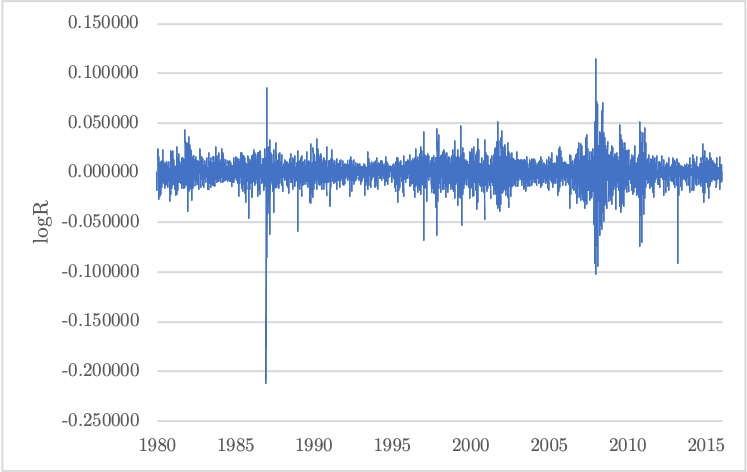
\includegraphics[width=9cm,height=5cm]{NYSE-Returns.png}
		\caption{NYSE Composite Index Daily Returns}
	\end{center}
	\end{figure}

	Figure 1 highlights relevant trends in the NYSE. Returns maintain fairly consistent volatility around a zero-mean with only a few large skews. The first of these is a combination of the 1985-1991 period of the Cold War against the Soviet Union and the 1987 market crash. Abnormally low returns are present in response to the rise of Mikhail Gorbachev and the arms race with President Reagan’s United States. The US’s victory over the communists saw strong recovery by the mid-90’s. Further, the 1987 foreign trade and exchange agreements, such as the Plaza Accord, aided daily returns of as low as \~{}-21\%. This may have led to the lowest NYSE returns of this period by over 100\% but again, recovery was fast. The crisis of the 90’s is also clearly reflected; along with the highly volatile 2007-2009, doubling return volatility.\\

	\begin{figure}[H]
        \begin{center}
                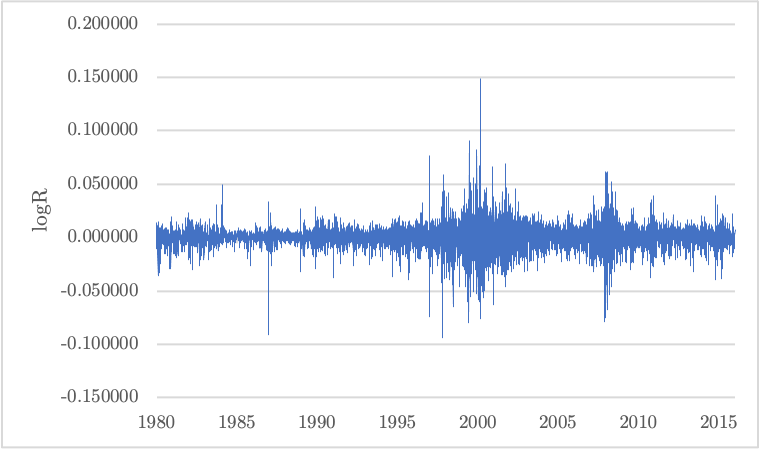
\includegraphics[width=9cm,height=5cm]{NASDAQ-Returns.png}
                \caption{NASDAQ Composite Index Daily Returns}
        \end{center}
        \end{figure}

	The NASDAQ (Figure 2) follows firms which react differently to social and economic states. Hence, different trends. The technology-based Dot-Com bubble of 1995-2004 offers the greatest abnormal return of \~{}15\%; almost 50\% greater than the NYSE’s and S\&P’s highest. Hence, NASDAQ is the best for risky investors. In the 2007-2009 crisis, the lowest skew is only \~{}75\% of the same point at the same time on the NYSE. Returns have normalised with consistent volatility around zero-mean.\\

	\begin{figure}[H]
        \begin{center}
		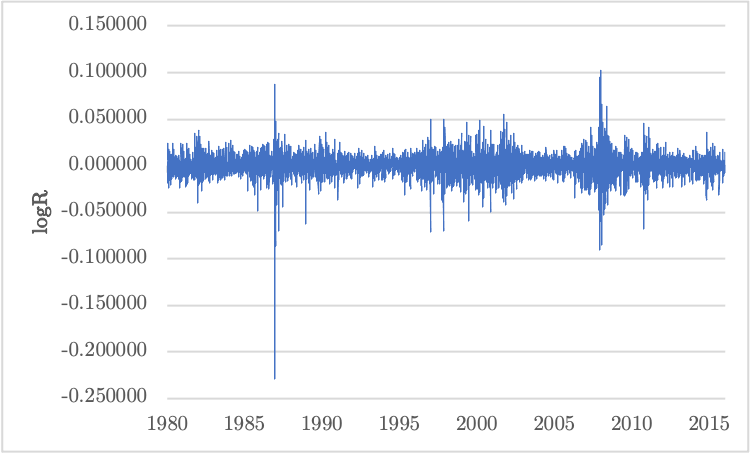
\includegraphics[width=9cm,height=5cm]{S&P-Returns.png}
		\caption{S\&P 500 Daily Returns}
        \end{center}
        \end{figure}
	
	Figure 3 shows consistent trends with the NYSE as many of the S\&P’s 500 firms are listed on the NYSE, not the NASDAQ or Cboe. However, the S\&P 500 fails to capture the negative abnormal returns of the 2013 debt crisis where the Obama Administration campaigned for higher minimum debt-raising through bond issuance. The NYSE does however, meaning that smaller firms were impacted more by this.

	\newpage 

	\subsection{Results Summary}

	\begin{table}[h]
		\scriptsize
	\begin{center}
	\begin{tabular}{ p{0.5cm}| p{0.5cm}| p{0.5cm}| p{0.5cm}| p{0.5cm}| p{0.5cm}| p{0.5cm}| p{0.5cm}| p{0.5cm}| p{0.5cm}| p{0.5cm}| p{0.5cm}| p{0.5cm}| p{0.5cm}| p{0.5cm} }
		\hline
		\hline
		\multicolumn{15}{c}{\textbf{The Weekend Effect}}\\
		\hline
		\hline
		\multicolumn{5}{c|}{\textbf{NYSE Composite}} & \multicolumn{5}{c|}{\textbf{NASDAQ Composite}} & \multicolumn{5}{c}{\textbf{S\&P 500}}\\
		\hline
		\textbf{CP} & \textbf{P1} & \textbf{P2} & \textbf{P3} & \textbf{P4} & \textbf{CP} & \textbf{P1} & \textbf{P2} & \textbf{P3} & \textbf{P4} & \textbf{CP} & \textbf{P1} & \textbf{P2} & \textbf{P3} & \textbf{P4}\\
		\hline
		N & Y$^M$ & Y$^M$ & N & N & Y$^M$ & Y & N & N & N & N & Y$^M$ & Y$^M$ & N & N\\
		\hline
		\hline
		\multicolumn{15}{c}{\textbf{The January Effect}}\\
		\hline
		\hline
		\multicolumn{5}{c|}{\textbf{NYSE Composite}} & \multicolumn{5}{c|}{\textbf{NASDAQ Composite}} & \multicolumn{5}{c}{\textbf{S\&P 500}}\\  
                \hline
		\textbf{CP} & \textbf{P1} & \textbf{P2} & \textbf{P3} & \textbf{P4} & \textbf{CP} & \textbf{P1} & \textbf{P2} & \textbf{P3} & \textbf{P4} & \textbf{CP} & \textbf{P1} & \textbf{P2} & \textbf{P3} & \textbf{P4}\\
                \hline
		N & N & N & N & N & N & N & N & N & N & N & N & N & N & N\\
		\hline
                \hline
                \multicolumn{15}{c}{\textbf{The Holiday Effect}}\\
                \hline                                          
                \hline
                \multicolumn{5}{c|}{\textbf{NYSE Composite}} & \multicolumn{5}{c|}{\textbf{NASDAQ Composite}} & \multicolumn{5}{c}{\textbf{S\&P 500}}\\  
                \hline
                \textbf{CP} & \textbf{P1} & \textbf{P2} & \textbf{P3} & \textbf{P4} & \textbf{CP} & \textbf{P1} & \textbf{P2} & \textbf{P3} & \textbf{P4} & \textbf{CP} & \textbf{P1} & \textbf{P2} & \textbf{P3} & \textbf{P4}\\
                \hline
		\multicolumn{15}{c}{\textbf{Standard}}\\
		\hline
		Y$^P$ & N & N & N & N & Y$^P$ & Y$^P$ & Y$^P$ & N & Y$^P$ & N & N & N & N & N\\
		\hline
		\multicolumn{15}{c}{\textbf{Omitting Pre-Holiday Fridays}}\\
		\hline
		Y$^P$ & Y$^S$ & N & N & N & N & N & N & N & N & Y$^{P-}$ & N & Y$^{P-}$ & N & N\\
		\hline
		\multicolumn{15}{c}{\textbf{Omitting Winter Weekends}}\\ 
                \hline
		Y$^P$ & N & N & N & N & Y$^P$ & Y$^P$ & N & N & N & N & N & N & N & N\\
		\hline
		\multicolumn{15}{c}{\textbf{Omitting Christmas Days}}\\    
                \hline
		Y$^P$ & N & N & N & N & Y$^P$ & Y$^P$ & N & N & N & N & N & N & N & N\\
		\hline
                \multicolumn{15}{c}{\textbf{Omitting New Year's Days}}\\ 
                \hline
                Y$^P$ & N & N & N & N & Y$^P$ & Y$^P$ & N & N & N & Y$^P$ & N & N & N & N\\
		\hline
		\multicolumn{15}{l}{CP: Comprehensive Period; P1: 1980-1989; ...; P4: 2010-2016}\\
		\multicolumn{15}{l}{Y: Evidence Exists; N: Evidence Does Not Exist (at the 5\% Significance Level)}\\ 
		\multicolumn{15}{l}{$^M$: Monday Effect Only; $^F$: Friday Effect Only}\\
		\multicolumn{15}{l}{$^P$: Pre-Holiday Effect Only; $^S$: Post-Holiday Effect Only; $^{(-)}$: Inverse of Effect}\\
		\hline
	\end{tabular}
		\caption{Evidential Summary of Seasonal Effects}
	\end{center}
	\end{table}

	As part of a comprehensive overview (Table 5.9), the Monday Effect exists in 40\% of the NYSE periods, 20\% of the NASDAQ periods, and 40\% of the S\&P 500 periods. The January Effect is only present at one period from 1990-1999 in the NASDAQ. The standard Holiday Effect is present in as the pre-holiday effect over the NYSE’s comprehensive period. Just the pre-holiday effect is present in 80\% of the observations over the NASDAQ. It’s not present at all in the S\&P 500. Omitting pre-holiday Fridays, 1990-1999 NYSE post-holiday days significantly different from the new mean but in the opposite direction; discussed latterly. The aforementioned 80\% pre-holiday effect in the NASDAQ is fully eliminated with the removal of pre-holiday Fridays. In the S\&P 500, the pre-holiday effect becomes apparent in two of the periods. Removal of winter weekends sees NYSE results remain the same; the NASDAQ sees the loss of pre-holiday significance in 1990-1999 and 2010-2016; the S\&P remains unchanged. Removal of Christmas Days again has no significant effect on the NYSE; the same occurs again with the loss of two significant periods in the NASDAQ and no change in the S\&P. Finally, removal of New Year’s Days has the same effect on the NYSE and NASDAQ as prior, a comprehensive pre-holiday significance arises in the S\&P.

	\newpage

	\subsection{The Weekend Effect}

		\subsubsection{The NYSE Composite Index}

	\begin{figure}[H]
        \begin{center}
                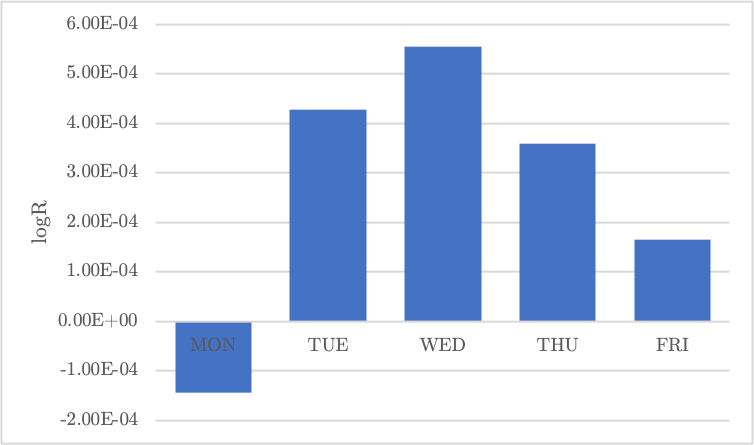
\includegraphics[width=9cm,height=5cm]{NYSE-WE1.png}
                \caption{NYSE Comprehensive Weekend Effect Mean Daily Returns}
        \end{center}
        \end{figure}

	Figure 4 shows partial evidence of the Monday Effect in the NYSE as a whole, highlighting that from 1980-2016 Monday returns are on average below zero. Their magnitude (of negativity) is however the lowest; roughly 7\% lower than the next smallest, Friday. Coincidently, meaning the Friday Effect is not apparent as Friday returns are the lowest positive ones; at less than 50\% of the value of the next lowest, Thursday. Wednesdays however, experience the highest returns by \~{}32\% to the next- in-line, Tuesdays. This enforces Yan-Ki’s (1990) idea that Wednesdays may see higher returns due to, the formerly discussed, settlement cost logistics. In result, the Weekend Effect is minorly supported but not potent.

	\begin{figure}[H]        
        \begin{center}
                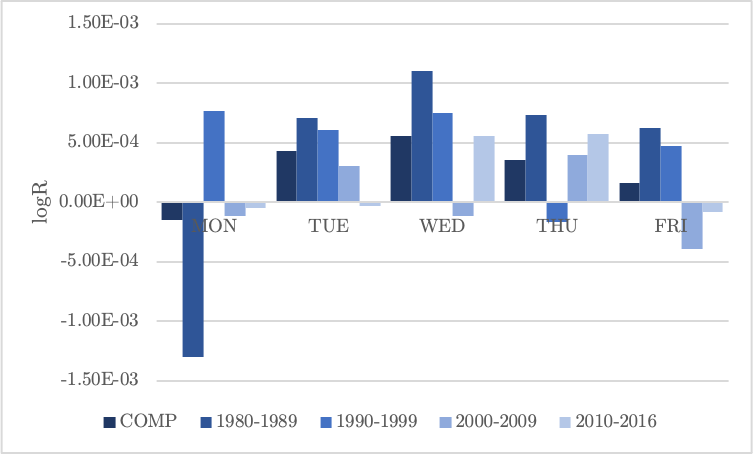
\includegraphics[width=9cm,height=5cm]{NYSE-WE2.png}    
                \caption{NYSE Segmented Weekend Effect Mean Daily Returns} 
        \end{center}
        \end{figure}

	Figure 5 segments mean weekly returns in the NYSE, displaying alterations over time. Evidently, Monday’s negative returns are primarily driven by 1980-1989 where they not only experience the lowest values by \~{}1175\% compared to 2000-2009’s but also, the highest magnitude of all observations by \~{}21.4\%, compared to 1980-1989’s high Wednesday returns; making them more negative than the highest positive observations are positive. Mondays experience high average returns from 1990-1999, being greater than any of the highest Tuesday, Thursday or Friday observations; contradicting the Monday Effect. Fridays also contradict the Friday Effect as their returns are negative in 2000-2009/2010-2016; with their greatest negativity more negative than those of any others apart from the 1980-1989 Mondays. They are, in no period, greater than all other days’.

	\newpage

	\begin{table}[h]
		\scriptsize
	\begin{center}
	\begin{tabular}{ p{2cm} p{2cm} p{2cm} p{2cm} p{2cm} }
		& \textbf{coefficient} & \textbf{std.err} & \textbf{t-ratio} & \textbf{p-value}\\
		\hline
		\multicolumn{5}{c}{\textbf{Section I: Comprehensive}}\\
		\hline
		Monday & & & & \\
		Tuesday & & & & \\
		Wednesday & & & & \\
		Thursday & & & & \\
		Friday & & & & \\
		\hline
		\multicolumn{5}{c}{\textbf{Section II: 1980--1989}}\\
		\hline            
                Monday & & & & \\   
                Tuesday & & & & \\  
                Wednesday & & & & \\
                Thursday & & & & \\
                Friday & & & & \\                                  
                \hline                                             
                \multicolumn{5}{c}{\textbf{Section III: 1990--1999}}\\
		\hline            
                Monday & & & & \\   
                Tuesday & & & & \\  
                Wednesday & & & & \\
                Thursday & & & & \\
                Friday & & & & \\                                  
                \hline                                             
                \multicolumn{5}{c}{\textbf{Section IV: 2000--2009}}\\
		\hline            
                Monday & & & & \\   
                Tuesday & & & & \\  
                Wednesday & & & & \\
                Thursday & & & & \\
                Friday & & & & \\                                  
                \hline                                             
                \multicolumn{5}{c}{\textbf{Section V: 2010--2016}}\\
		\hline
		Monday & & & & \\                               
                Tuesday & & & & \\                              
                Wednesday & & & & \\
                Thursday & & & & \\
                Friday & & & & \\                                  
                \hline
		\multicolumn{5}{l}{$^*$: 10\% Significance Level}\\
		\multicolumn{5}{l}{$^{**}$: 5\% Significance Level}\\
		\multicolumn{5}{l}{$^{***}$: 1\% Significance Level}\\
		\hline
	\end{tabular}
		\caption{NYSE Weekend Effect Regression Results}
	\end{center}
	\end{table}

	Table 5.10 reinforces prior arguments, showing negative Mondays returns, at the 1\% significance level, in 1980-1989; with a coefficient stating that a Monday results in an average lower return by 0.000158 units, over any other day. Monday returns are positive at the 5\% significance level in 1990-1999. Wednesday’s 1980-1989 highest- across-the-board returns are too, significantly positive; with a coefficient stating that a Wednesday results in an average higher return by 0.001064 units in 1980-1989, over any other day. However, there is no significance on even the most positive Fridays. Hence, the null hypothesis that the investigated day’s return is approximately equal to those of other days is only rejected, with 99\% confidence, for 1980-1989 Mondays in favour of them being significantly lower. Thus, the Weekend Effect is not apparent in the NYSE from 1980-2016 but, the Monday Effect is present in 1980-1989.

		\subsubsection{The NASDAQ Composite Index}

	\begin{figure}[H]
        \begin{center}
                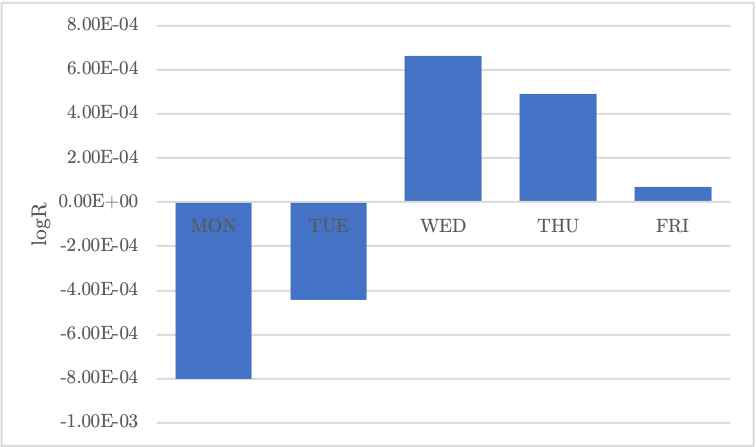
\includegraphics[width=9cm,height=5cm]{NAS-WE1.png}
                \caption{NASDAQ Comprehensive Weekend Effect Mean Daily Returns}
        \end{center}
        \end{figure}

	Figure 6 highlights more evident negative Monday returns on the NASDAQ, being \~{}100\% lower than those of Tuesday’s and \~{}430\% lower than those of the NYSE’s. Wednesdays again experience the highest returns, this time \~{}34\% greater than next highest, Thursdays. Fridays are positive but least so of all, at just \~{}10\% of Thursdays; contradicting the Friday effect.

	\begin{figure}[H]
        \begin{center}
                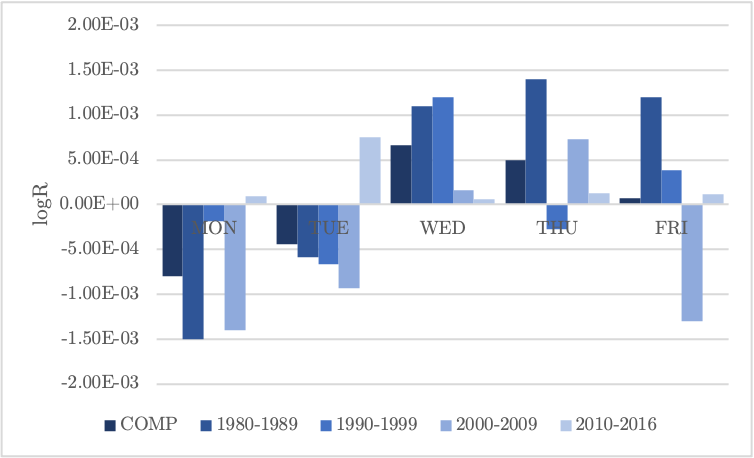
\includegraphics[width=9cm,height=5cm]{NAS-WE2.png} 
                \caption{NASDAQ Segmented Weekend Effect Mean Daily Returns}
        \end{center}
        \end{figure}
		
	Figure 7 shows the NASDAQ supports the Monday Effect stronger than the NYSE, primarily due to 1980-1989/2000-2009’s very low Monday returns. 1980-1989’s Mondays hold the lowest returns with the highest magnitude by \~{}7\%, compared to those of Thursday’s 1980-1989 highest-across-the-board – which have roughly the same magnitude as 2000-2009’s negative Mondays. A similar trend is apparent in the NYSE. The only positive Monday returns are in 2010-2016, even then they hold the second-lowest positive value and second-lowest overall magnitude. This time, Fridays do hold the highest returns, in 1980-1989; supporting the Friday Effect, but only by \~{}16\% over the same period’s Wednesdays. However this is the only period of high Friday returns; 2000-2009 shows almost as negative Fridays as its Mondays.

	\begin{table}[h]
                \scriptsize
        \begin{center}
        \begin{tabular}{ p{2cm} p{2cm} p{2cm} p{2cm} p{2cm} }
                & \textbf{coefficient} & \textbf{std.err} & \textbf{t-ratio} & \textbf{p-value}\\
                \hline
                \multicolumn{5}{c}{\textbf{Section I: Comprehensive}}\\
                \hline
                Monday & & & & \\
                Tuesday & & & & \\
                Wednesday & & & & \\
                Thursday & & & & \\
                Friday & & & & \\
                \hline
                \multicolumn{5}{c}{\textbf{Section II: 1980--1989}}\\
                \hline            
                Monday & & & & \\   
                Tuesday & & & & \\  
                Wednesday & & & & \\
                Thursday & & & & \\
                Friday & & & & \\                                  
                \hline                                             
                \multicolumn{5}{c}{\textbf{Section III: 1990--1999}}\\
                \hline            
                Monday & & & & \\   
                Tuesday & & & & \\  
                Wednesday & & & & \\
                Thursday & & & & \\
                Friday & & & & \\                                  
                \hline                                             
                \multicolumn{5}{c}{\textbf{Section IV: 2000--2009}}\\
                \hline            
                Monday & & & & \\   
                Tuesday & & & & \\  
                Wednesday & & & & \\
                Thursday & & & & \\
                Friday & & & & \\                                  
                \hline                                             
                \multicolumn{5}{c}{\textbf{Section V: 2010--2016}}\\
                \hline
                Monday & & & & \\                               
                Tuesday & & & & \\                              
                Wednesday & & & & \\
                Thursday & & & & \\
                Friday & & & & \\                                  
                \hline
                \multicolumn{5}{l}{$^*$: 10\% Significance Level}\\
                \multicolumn{5}{l}{$^{**}$: 5\% Significance Level}\\
                \multicolumn{5}{l}{$^{***}$: 1\% Significance Level}\\
                \hline
        \end{tabular}
                \caption{NASDAQ Weekend Effect Regression Results}
        \end{center}
        \end{table}

	Table 5.11 highlights more significance in the NASDAQ than the NYSE. Monday returns are significantly negative at the 1\% level in 1980-1989 with a coefficient stating a Monday results in a lower average return of 0.001623 units, over other days. 1980- 1989 primarily contributes to the 1\% significance in the overall period. Although 2000-2009 Monday returns hold low significance, they are only significant at the 10\% level so are ignored. 1990-1999 Wednesday returns are significantly positive at the 1\% level, with a coefficient stating that a Wednesday results in a higher return of 0.000161 units, over any other day. This aligns with Figure 8 showing highest Wednesday returns in this period. 1980-1989 Wednesdays present the same positive significance. Fridays are significantly positive only in 1980-1989 but at the 1\% level; stating a Friday results in an average higher return 0.001247 units, over any other day. The null hypothesis of observed days’ returns being roughly equal to those of others is rejected with 99\% confidence for comprehensive/1980-1989 Mondays and, for Fridays at the same level in 1980-1989. Thus, the Weekend Effect is present in 1980-1989 but comprehensively, only the Monday Effect is present.

		\subsubsection{The S\&P 500}

	\begin{figure}[H]
        \begin{center}
                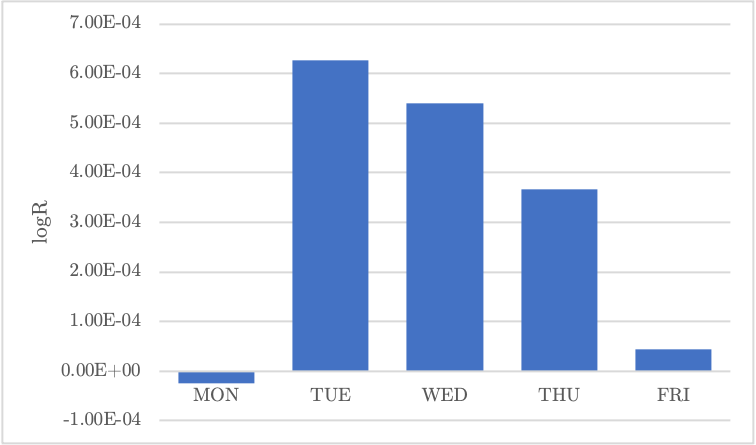
\includegraphics[width=9cm,height=5cm]{SP-WE1.png}
		\caption{S\&P 500 Comprehensive Weekend Effect Mean Daily Returns}
        \end{center}
        \end{figure}

	Figure 8 shows similar results in the S\&P 500 to the NYSE with regards to the taper from high to low; Wednesday-Friday. Average Monday returns are below zero however, again have the lowest magnitude by \~{}100\% so are not observably very negative. Their magnitude is only \~{}14\% of those of the NYSE; the originally negative but insignificant Mondays. Tuesdays however, hold the highest average for the first time, by \~{}17\% Fridays again, are the lowest at only \~{}11\% of next-highest, Thursday.

	\begin{figure}[H]
        \begin{center}
                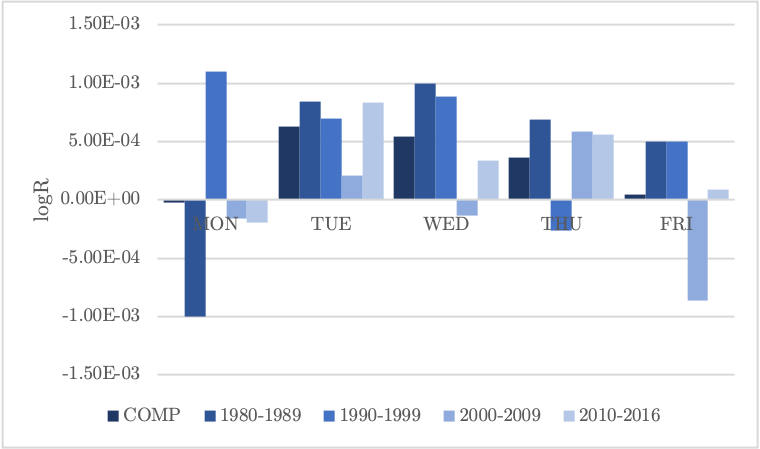
\includegraphics[width=9cm,height=5cm]{SP-WE2.png} 
                \caption{S\&P 500 Segmented Weekend Effect Mean Daily Returns}
        \end{center}
        \end{figure}
	
	Figure 9 sees the comprehensive period’s almost-zero Monday mean originate from 1980-1989 and 1990-1999 Monday returns almost having an identical magnitude; the latter is slightly more positive than the former is negative. Overall, they are drawn back to the negative by the consistent, but low, negativity in 2000-2009/2010-2016. 1980-1989 Mondays are more negative than any other observation by \~{}33\% compared to the next-most-negative, 2000-2009 Fridays. So, the Monday Effect is supported. 2000-2009 very low Fridays are apparent across all indices and contradict the Friday Effect. Friday returns do not exceed any other day’s returns at any period, also contradicting the Friday Effect.

	\newpage

	\begin{table}[h]
                \scriptsize
        \begin{center}
        \begin{tabular}{ p{2cm} p{2cm} p{2cm} p{2cm} p{2cm} }
                & \textbf{coefficient} & \textbf{std.err} & \textbf{t-ratio} & \textbf{p-value}\\
                \hline
                \multicolumn{5}{c}{\textbf{Section I: Comprehensive}}\\
                \hline
                Monday & & & & \\
                Tuesday & & & & \\
                Wednesday & & & & \\
                Thursday & & & & \\
                Friday & & & & \\
                \hline
                \multicolumn{5}{c}{\textbf{Section II: 1980--1989}}\\
                \hline            
                Monday & & & & \\   
                Tuesday & & & & \\  
                Wednesday & & & & \\
                Thursday & & & & \\
                Friday & & & & \\                                  
                \hline                                             
                \multicolumn{5}{c}{\textbf{Section III: 1990--1999}}\\
                \hline            
                Monday & & & & \\   
                Tuesday & & & & \\  
                Wednesday & & & & \\
                Thursday & & & & \\
                Friday & & & & \\                                  
                \hline                                             
                \multicolumn{5}{c}{\textbf{Section IV: 2000--2009}}\\
                \hline            
                Monday & & & & \\   
                Tuesday & & & & \\  
                Wednesday & & & & \\
                Thursday & & & & \\
                Friday & & & & \\                                  
                \hline                                             
                \multicolumn{5}{c}{\textbf{Section V: 2010--2016}}\\
                \hline
                Monday & & & & \\                               
                Tuesday & & & & \\                              
                Wednesday & & & & \\
                Thursday & & & & \\
                Friday & & & & \\                                  
                \hline
                \multicolumn{5}{l}{$^*$: 10\% Significance Level}\\
                \multicolumn{5}{l}{$^{**}$: 5\% Significance Level}\\
                \multicolumn{5}{l}{$^{***}$: 1\% Significance Level}\\
                \hline
        \end{tabular}
		\caption{S\&P 500 Weekend Effect Regression Results}
        \end{center}
        \end{table}

	Table 5.12 highlights similar significance to the NYSE, seeing that Mondays in 1980- 1989 are negative at the 5\% significance level; with a coefficient stating that Mondays result in a lower average return of 0.00105 units, in comparison to those of other days. As expected, 1990-1999 Monday returns are significantly positive at the 1\% level thus, more significantly positive than 1980-1989’s are negative. Their coefficient shows a 1990-1999 Monday would on average result in a higher return of 0.001083 units, over other days. Comprehensively, Tuesdays and Wednesdays are significantly positive, driven by positivity in 1980-1989/1990-1999. However, there are no significantly positive Friday periods. The null hypothesis is rejected with 99\% confidence only for Mondays in 1980-1989. Thus, no Weekend Effect is present. The Monday Effect is supported from 1980-1989.

	\newpage

	\subsection{The January Effect}

		\subsubsection{The NYSE Composite Index}

	\begin{figure}[H]
        \begin{center}
                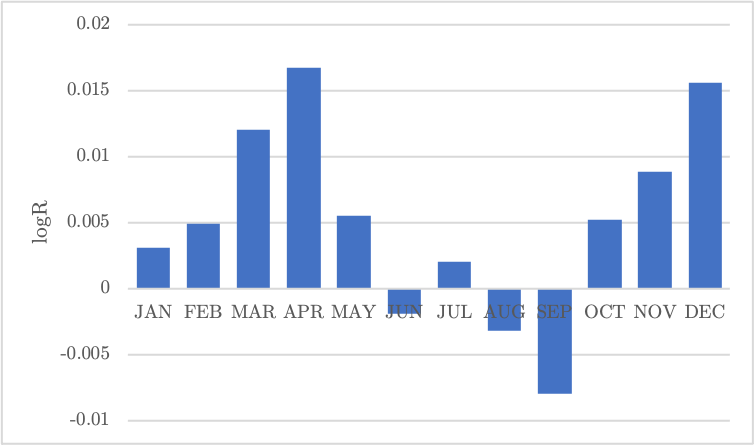
\includegraphics[width=9cm,height=5cm]{NYSE-JE1.png} 
                \caption{NYSE Comprehensive January Effect Mean Daily Returns}
        \end{center}
        \end{figure}

	Immediately, it’s apparent from Figure 10 that the January Effect is irrelevant in the NYSE on-a-whole. January’s average return is the second lowest positive, with the lowest only being \~{}1e-3 units lower. Its magnitude is also the second lowest, when comparing to the negative months. Highest returns occur in April, by \~{}1.3\% over the next-highest, December and; by \~{}665\% over the lowest positive, July. This December value contradicts Rozeff \& Kinney’s (1976) idea that December returns are often low in anticipation of the new year.

	\begin{figure}[H]
        \begin{center}
                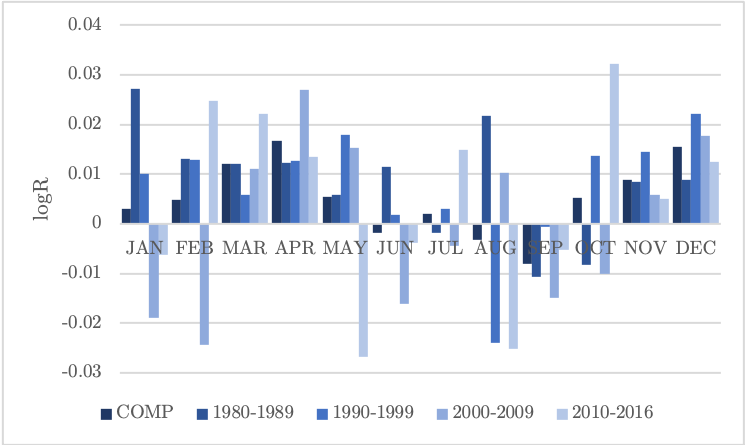
\includegraphics[width=9cm,height=5cm]{NYSE-JE2.png}
                \caption{NYSE Segmented January Effect Mean Daily Returns}     
        \end{center}
        \end{figure}

	Figure 11 shows that the reasoning for comprehensive low average January return is found in 2000-2009 where January experiences the fifth most negative returns across- the-board. 1980-1989 however, does see January returns higher than those of all other months; by \~{}120\% compared to next-in-line, February. This trend is not repeated however. March, April, November and December returns are the most reliable with no negative averages; all being consistently and highly positive. Summer months remain deviating roughly the same both positively and negatively from zero. October experiences the highest skew with the greatest magnitude (both positive and negative) of average return.

	\begin{center}
		\scriptsize
	\begin{longtable}{ p{2cm} p{2cm} p{2cm} p{2cm} p{2cm} }
		& \textbf{coefficient} & \textbf{std.err} & \textbf{t-ratio} & \textbf{p-value}\\
		\hline
		\multicolumn{5}{c}{\textbf{Section I: Comprehensive}}\\
		\hline
		January & & & & \\
		February & & & & \\
		March & & & & \\
		April & & & & \\
		May & & & & \\
		June & & & & \\
		July & & & & \\
		August & & & & \\
		September & & & & \\
		October & & & & \\
		November & & & & \\
		December & & & & \\
		\hline
		\multicolumn{5}{c}{\textbf{Section II: 1980--1989}}\\
		\hline
		January & & & & \\                              
                February & & & & \\
                March & & & & \\
                April & & & & \\
                May & & & & \\
                June & & & & \\
                July & & & & \\
                August & & & & \\
                September & & & & \\
                October & & & & \\
                November & & & & \\
                December & & & & \\
                \hline
                \multicolumn{5}{c}{\textbf{Section III: 1990--1999}}\\ 
		\hline
                January & & & & \\
                February & & & & \\                             
                March & & & & \\
                April & & & & \\
                May & & & & \\
                June & & & & \\
                July & & & & \\
                August & & & & \\
                September & & & & \\
                October & & & & \\
                November & & & & \\
                December & & & & \\
                \hline
                \multicolumn{5}{c}{\textbf{Section IV: 2000--2009}}\\
		\hline
                January & & & & \\
                February & & & & \\                             
                March & & & & \\
                April & & & & \\
                May & & & & \\
                June & & & & \\
                July & & & & \\
                August & & & & \\
                September & & & & \\
                October & & & & \\
                November & & & & \\
                December & & & & \\
                \hline
                \multicolumn{5}{c}{\textbf{Section V: 2010--2016}}\\
		\hline
		January & & & & \\
                February & & & & \\                             
                March & & & & \\
                April & & & & \\
                May & & & & \\
                June & & & & \\
                July & & & & \\
                August & & & & \\
                September & & & & \\
                October & & & & \\
                November & & & & \\
                December & & & & \\
		\hline
		\multicolumn{5}{l}{$^*$: 10\% Significance Level}\\
                \multicolumn{5}{l}{$^{**}$: 5\% Significance Level}\\
                \multicolumn{5}{l}{$^{***}$: 1\% Significance Level}\\
		\hline
		\caption{NYSE January Effect Regression Results}
	\end{longtable}
	\end{center}

	Table 5.13 shows that no January observations were significantly positive at the 5\% level; with only 1980-1989/1990-1999’s being significant at the 10\% level. Therefore, the null hypothesis that the observed month’s returns are approximately equal to those of others is failed-to-be-rejected. Thus, the January Effect is not present at any observed period in the NYSE. As expected however, the null is rejected with 95\% confidence for 2010-2016 October highly positive skew; with a coefficient stating October results in a higher average return of 0.03221 units, over those other months. Also in-line with charts, 1990-1999’s April and December returns are respectively significantly low and high, both at the 5\% significance level; rejecting the null with 95\% confidence.
	
		\subsubsection{The NASDAQ Composite Index}

	\begin{figure}[H]
        \begin{center}
                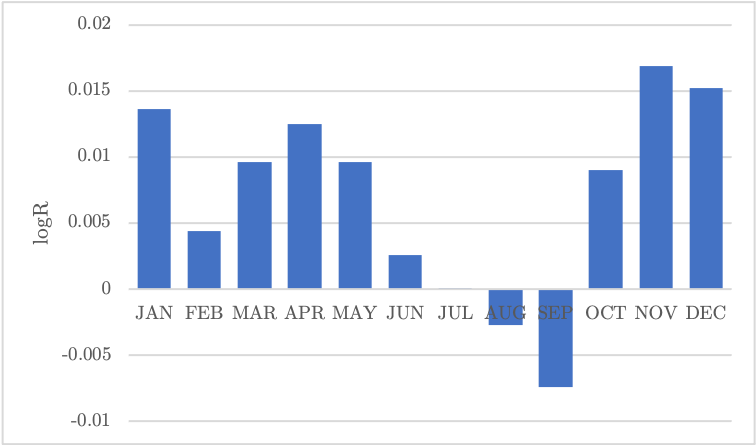
\includegraphics[width=9cm,height=5cm]{NAS-JE1.png} 
                \caption{NASDAQ Comprehensive January Effect Mean Daily Returns}
        \end{center}
        \end{figure}

	Figure 12 shows that the NASDAQ is generally more in favour of the January Effect as its comprehensive January average is \~{}460\% greater than that of the NYSE. They are also the third-highest; just \~{}7\% under second, December. But, are clearly not greater than all other months on-a-whole, which is contradictory to the January Effect. There are no significant observations; monthly returns are consistently high across the NASDAQ with only July/August/September being \~{}0/negative. Their magnitudes are low compared to other months however, so aren’t excessively negative.

	\begin{figure}[H]
        \begin{center}
                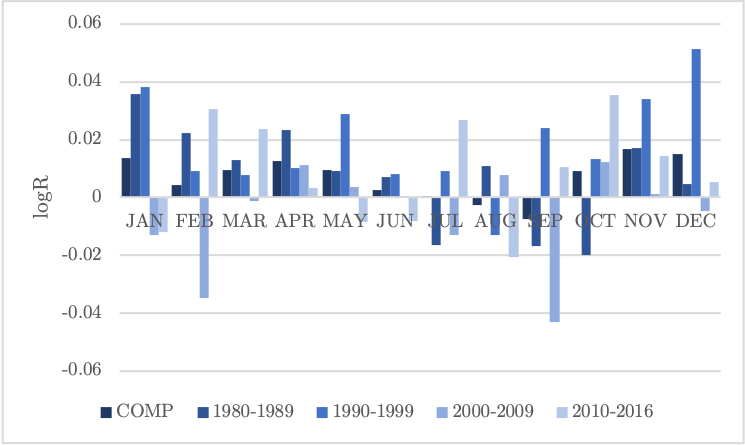
\includegraphics[width=9cm,height=5cm]{NAS-JE2.png}  
                \caption{NASDAQ Segmented January Effect Mean Daily Returns}
        \end{center}
        \end{figure}

	Figure 13 shows that 1980-1989 Januarys support the January Effect as the January average is higher than all others. This trend doesn’t hold however. It is close in 1990-1999 where the average December return is the only one larger, by \~{}25\%. The remainder of January means are negative; contradicting the January Effect. Much like the NYSE, March, April, May and November experience consistently positive returns, with their, few, negative’s magnitudes being low. Summer months deviate consistently.

	\begin{center}
                \scriptsize
        \begin{longtable}{ p{2cm} p{2cm} p{2cm} p{2cm} p{2cm} }
                & \textbf{coefficient} & \textbf{std.err} & \textbf{t-ratio} & \textbf{p-value}\\
                \hline
                \multicolumn{5}{c}{\textbf{Section I: Comprehensive}}\\
                \hline
                January & & & & \\
                February & & & & \\
                March & & & & \\
                April & & & & \\
                May & & & & \\
                June & & & & \\
                July & & & & \\
                August & & & & \\
                September & & & & \\
                October & & & & \\
                November & & & & \\
                December & & & & \\
                \hline
                \multicolumn{5}{c}{\textbf{Section II: 1980--1989}}\\
                \hline
                January & & & & \\                              
                February & & & & \\
                March & & & & \\
                April & & & & \\
                May & & & & \\
                June & & & & \\
                July & & & & \\
                August & & & & \\
                September & & & & \\
                October & & & & \\
                November & & & & \\
                December & & & & \\
                \hline
		\multicolumn{5}{c}{\textbf{Section III: 1990--1999}}\\ 
                \hline
                January & & & & \\
                February & & & & \\                             
                March & & & & \\
                April & & & & \\
                May & & & & \\
                June & & & & \\
                July & & & & \\
                August & & & & \\
                September & & & & \\
                October & & & & \\
                November & & & & \\
                December & & & & \\
                \hline
                \multicolumn{5}{c}{\textbf{Section IV: 2000--2009}}\\
                \hline
                January & & & & \\
                February & & & & \\                             
                March & & & & \\
                April & & & & \\
                May & & & & \\
                June & & & & \\
                July & & & & \\
                August & & & & \\
                September & & & & \\
                October & & & & \\
                November & & & & \\
                December & & & & \\
                \hline
                \multicolumn{5}{c}{\textbf{Section V: 2010--2016}}\\ 
                \hline 
                January & & & & \\
                February & & & & \\                             
                March & & & & \\
                April & & & & \\
                May & & & & \\
                June & & & & \\
                July & & & & \\
                August & & & & \\
                September & & & & \\
                October & & & & \\
                November & & & & \\
                December & & & & \\
                \hline                                             
                \multicolumn{5}{l}{$^*$: 10\% Significance Level}\\  
                \multicolumn{5}{l}{$^{**}$: 5\% Significance Level}\\ 
                \multicolumn{5}{l}{$^{***}$: 1\% Significance Level}\\
                \hline                                          
                \caption{NASDAQ January Effect Regression Results}
        \end{longtable}
        \end{center}

	Table 5.14 shows that the only period worth observing regarding the January Effect is 1990-1999. January is positive at the 1\% significance level; with a coefficient stating January results in a higher average return of 0.05373, over other months. December is also significant at this level; with a coefficient stating December results in a higher average return of 0.0512, over other months. 2010-2016’s October is also significantly positive at the 5\% level. Most importantly, the null hypothesis that the observed month’s returns are approximately equal to those of others is rejected with 99\% confidence for both January and December in 1990-1999, meaning the January Effect exists in the 1990-1999 period. Furthermore, as the coefficient of January is greater, it is likely there are more frequent January Effect skews within the period but December returns are on average higher. As, observing 1990-1999 (Figure 13), December’s average is greater; contradicting the January Effect.

		\subsubsection{The S\&P 500}

	\begin{figure}[H]
        \begin{center}
                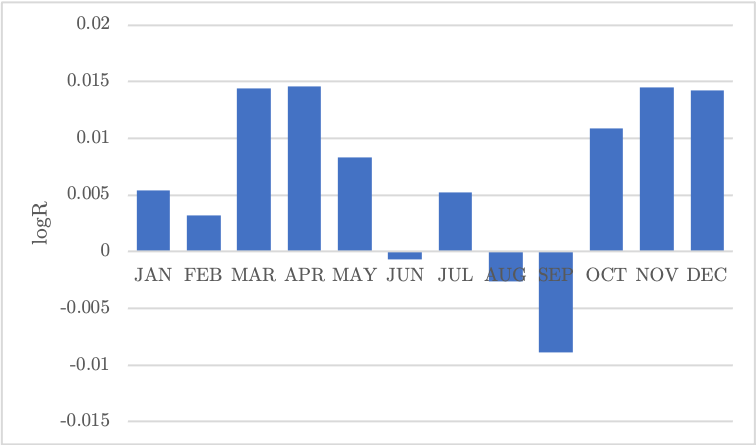
\includegraphics[width=9cm,height=5cm]{SP-JE1.png} 
		\caption{S\&P 500 Comprehensive January Effect Mean Daily Returns}
        \end{center}
        \end{figure}	

	Figure 14 highlights similarity with the NYSE where January’s average return is the third lowest on-a-whole, being just \~{}2.25e-3 units higher than the lowest, initially contradicting the January Effect. Roughly equivalent high returns are observed across March-May; October-December. Summer months, as consistent with other indices, are the lowest and most negative. The greatest magnitude is seen on a positive however; April.

	\begin{figure}[H]
        \begin{center}
                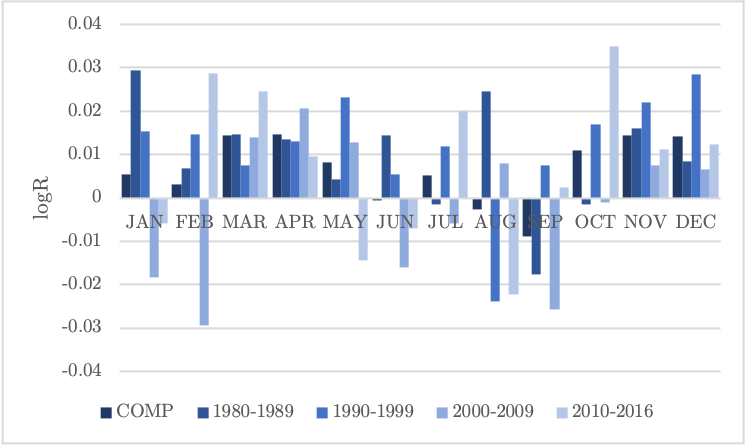
\includegraphics[width=9cm,height=5cm]{SP-JE2.png}  
                \caption{S\&P 500 Segmented January Effect Mean Daily Returns}
        \end{center}
        \end{figure}

	Figure 15 again shows consistency with other indices in that January returns are highest in 1980-1989/1990-1999 but negative in 2000-2009/2010-2016. January’s 1980- 1989 are greater than those of other months being \~{}22\% greater than next-in-line, August; in favour of the January Effect. It’s likely the 2000-2009 great negative January mean is what skewed the comprehensive January value to a low-lying positive. Spring and Autumn/Winter months are again consistently greater than zero, with summer months again seeing high-magnitude negative returns.

	\begin{center}
                \scriptsize
        \begin{longtable}{ p{2cm} p{2cm} p{2cm} p{2cm} p{2cm} }
                & \textbf{coefficient} & \textbf{std.err} & \textbf{t-ratio} & \textbf{p-value}\\
                \hline
                \multicolumn{5}{c}{\textbf{Section I: Comprehensive}}\\
                \hline
                January & & & & \\
                February & & & & \\
                March & & & & \\
                April & & & & \\
                May & & & & \\
                June & & & & \\
                July & & & & \\
                August & & & & \\
                September & & & & \\
                October & & & & \\
                November & & & & \\
                December & & & & \\
                \hline
                \multicolumn{5}{c}{\textbf{Section II: 1980--1989}}\\
                \hline
                January & & & & \\                              
                February & & & & \\
                March & & & & \\
                April & & & & \\
                May & & & & \\
                June & & & & \\
                July & & & & \\
                August & & & & \\
                September & & & & \\
                October & & & & \\
                November & & & & \\
                December & & & & \\
                \hline
		\multicolumn{5}{c}{\textbf{Section III: 1990--1999}}\\ 
                \hline
                January & & & & \\
                February & & & & \\                             
                March & & & & \\
                April & & & & \\
                May & & & & \\
                June & & & & \\
                July & & & & \\
                August & & & & \\
                September & & & & \\
                October & & & & \\
                November & & & & \\
                December & & & & \\
                \hline
                \multicolumn{5}{c}{\textbf{Section IV: 2000--2009}}\\
                \hline
                January & & & & \\
                February & & & & \\                             
                March & & & & \\
                April & & & & \\
                May & & & & \\
                June & & & & \\
                July & & & & \\
                August & & & & \\
                September & & & & \\
                October & & & & \\
                November & & & & \\
                December & & & & \\
                \hline
                \multicolumn{5}{c}{\textbf{Section V: 2010--2016}}\\ 
                \hline 
                January & & & & \\
                February & & & & \\                             
                March & & & & \\
                April & & & & \\
                May & & & & \\
                June & & & & \\
                July & & & & \\
                August & & & & \\
                September & & & & \\
                October & & & & \\
                November & & & & \\
                December & & & & \\
                \hline                                             
                \multicolumn{5}{l}{$^*$: 10\% Significance Level}\\  
                \multicolumn{5}{l}{$^{**}$: 5\% Significance Level}\\ 
                \multicolumn{5}{l}{$^{***}$: 1\% Significance Level}\\
                \hline                                          
		\caption{S\&P 500 January Effect Regression Results}
        \end{longtable}
        \end{center}

	Table 5.15 shows that although 1980-1989’s January mean is higher than other months’, it’s not significantly different. Therefore, the null that the observed month’s (January) returns are roughly equivalent to those of others is failed-to-be-rejected, finding no evidence of a significant January Effect. As expected though, some Spring/Autumn months are significant. For example, 2010-2016’s October is positive at the 1\% significance level. This aligns with Figure 15 as this month holds the highest magnitude across both positive and negative observations.

	\newpage

	\subsection{The Holiday Effect}

		\subsubsection{The NYSE Composite Index}

	\begin{figure}[H]
        \begin{center}
                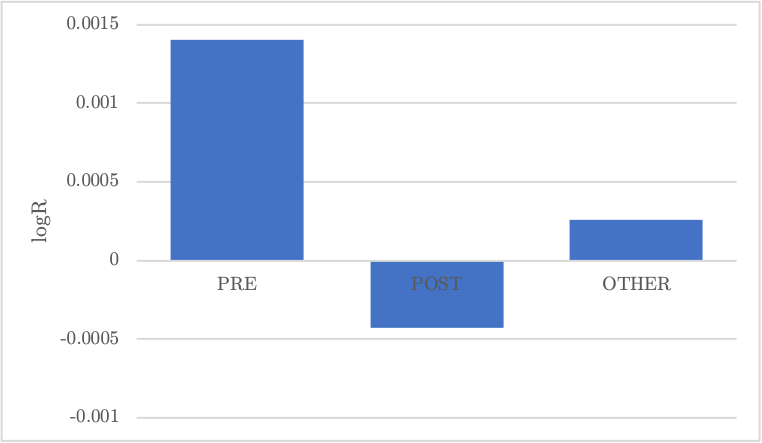
\includegraphics[width=9cm,height=5cm]{NYSE-HE1.png} 
                \caption{NYSE Comprehensive Holiday Effect Mean Daily Returns}
        \end{center}
        \end{figure}

	Figure 16 shows evidence of Holiday Effect theory. Pre-holiday days are, on-a-whole, the most positive by \~{}480\% over `other' days and; also has the greatest magnitude by \~{}220\%. Post-holiday days are also in support; showing the only negative mean.

	\begin{figure}[H]
        \begin{center}
                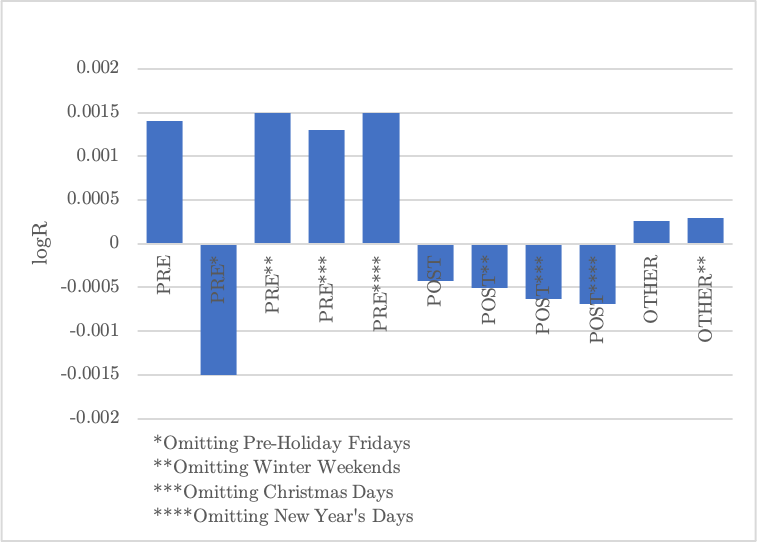
\includegraphics[width=9cm,height=5cm]{NYSE-HE2.png}              
		\caption{NYSE Comprehensive Holiday Effect Mean Daily Returns H.E.E.}
        \end{center}
        \end{figure}

	Figure 17 outlines the four extensions made to the Holiday Effect. When removing pre-holiday Fridays, pre-holiday returns experience a complete reverse around zero; they become \~{}10\% more negative than they were positive. This means most of the valuable pre-holiday days fall on Fridays. Omitting winter weekends sees pre-holiday returns increase by \~{}10\%, with post-holidays becoming more slightly negative. Other days remain roughly the same. This means winter weekends likely contain lower- return-than-average pre-holiday days and lower-return-than-average post-holiday days. Thus, suggesting winter weekends contain an `inverse Holiday Effect’. Removing Christmas sees pre-holiday days remain roughly the same but makes the post-holiday average more negative; suggesting higher post-holiday returns at Christmas. Removing New Year sees another \~{}10\% increase in pre-holiday mean and the biggest increase in negativity of post-holidays; having a similar effect to winter weekends in the `inverse Holiday Effect’ manner.

	\begin{figure}[H]
        \begin{center}
                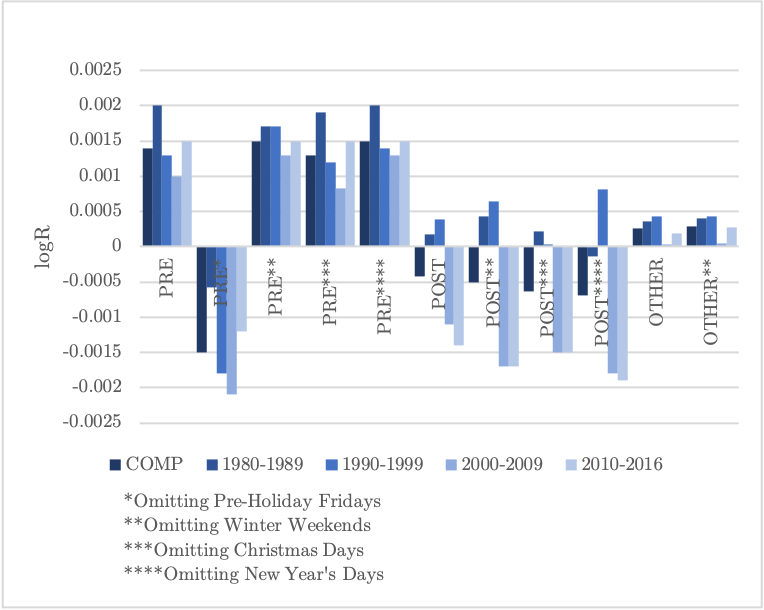
\includegraphics[width=9cm,height=5cm]{NYSE-HE3.png}              
                \caption{NYSE Segmented Holiday Effect Mean Daily Returns H.E.E.}    
        \end{center}
        \end{figure}

	Figure 18 generally supports previous arguments, when the NYSE is time-segmented. Pre-holiday returns are highest in 1980-1989 by \~{}60\%. They follow a generally high subsequent trend. The pre-holiday Friday removal `flip-effect’ carries over all periods but negativity increase is lowest (\~{}50\% of next-in-line) in 1980-1989, where returns were highest. This means most of the high-valued pre-holiday Fridays removed occurred after this period. Removal of winter weekends makes pre-holiday returns more consistent over-time; increasing all values but 1980-1989’s (which decreases), meaning the `inverse Holiday Effect’ occurs after 1980-1989. This is reflected in most of the increase in negativity in post-holiday days coming from the large 2000-2016 drops; further condensing the `inverse Holiday Effect’ to just 2000-2016. This effect also decreased `other days’ to near-zero meaning many of the higher-return winter weekends occurred on non-pre/post-holiday days. Removing Christmas consistently draws pre-holidays down aligning with higher-than-average pre-Christmas-holiday days but also consistent `inverse pre-holiday effect’ in that all post-holiday days become more negative meaning higher post-holiday days lie around Christmas. New Year holds the `inverse Holiday Effect’ (holding lower-than-average pre-holidays and higher-than-average post-holidays; increasing pre-holiday/decreasing post- holidays) in all periods but 1990-1999.

	\begin{center}
		\scriptsize
	\begin{longtable}{ p{2cm} p{2cm} p{2cm} p{2cm} p{2cm} }
		& \textbf{coefficient} & \textbf{std.err} & \textbf{t-ratio} & \textbf{p-value}\\
		\hline
		\hline
		\multicolumn{5}{c}{\textbf{Standard}}\\
		\hline
		\hline
		\multicolumn{5}{c}{\textbf{Section I: Comprehensive}}\\
		\hline
		Pre-Hol & & & & \\
		Post-Hol & & & & \\
		Other Days & & & & \\
		\hline
		\multicolumn{5}{c}{\textbf{Section II: 1980--1989}}\\
                \hline            
                Pre-Hol & & & & \\ 
                Post-Hol & & & & \\  
                Other Days & & & & \\
                \hline
		\multicolumn{5}{c}{\textbf{Section III: 1990--1999}}\\
                \hline            
                Pre-Hol & & & & \\ 
                Post-Hol & & & & \\  
                Other Days & & & & \\
                \hline
		\multicolumn{5}{c}{\textbf{Section IV: 2000--2009}}\\
                \hline            
                Pre-Hol & & & & \\ 
                Post-Hol & & & & \\  
                Other Days & & & & \\
                \hline
		\multicolumn{5}{c}{\textbf{Section V: 2010--2016}}\\
                \hline            
                Pre-Hol & & & & \\ 
                Post-Hol & & & & \\  
                Other Days & & & & \\
                \hline
                \hline                                 
                \multicolumn{5}{c}{\textbf{Omitting Pre-Holiday Fridays}}\\         
                \hline
                \hline                                                 
                \multicolumn{5}{c}{\textbf{Section I: Comprehensive}}\\
                \hline            
                Pre-Hol & & & & \\ 
                Post-Hol & & & & \\  
                Other Days & & & & \\
                \hline                                          
                \multicolumn{5}{c}{\textbf{Section II: 1980--1989}}\\   
                \hline            
                Pre-Hol & & & & \\ 
                Post-Hol & & & & \\  
                Other Days & & & & \\
                \hline 
                \multicolumn{5}{c}{\textbf{Section III: 1990--1999}}\\   
                \hline            
                Pre-Hol & & & & \\ 
                Post-Hol & & & & \\  
                Other Days & & & & \\
                \hline 
                \multicolumn{5}{c}{\textbf{Section IV: 2000--2009}}\\   
                \hline                                          
                Pre-Hol & & & & \\
                Post-Hol & & & & \\  
                Other Days & & & & \\
                \hline 
                \multicolumn{5}{c}{\textbf{Section V: 2010--2016}}\\   
                \hline            
                Pre-Hol & & & & \\ 
                Post-Hol & & & & \\  
                Other Days & & & & \\
                \hline
                \hline                                          
                \multicolumn{5}{c}{\textbf{Omitting Winter Weekends}}\\ 
                \hline
                \hline
                \multicolumn{5}{c}{\textbf{Section I: Comprehensive}}\\
                \hline
                Pre-Hol & & & & \\
                Post-Hol & & & & \\
                Other Days & & & & \\
                \hline
                \multicolumn{5}{c}{\textbf{Section II: 1980--1989}}\\
                \hline
                Pre-Hol & & & & \\
                Post-Hol & & & & \\  
                Other Days & & & & \\
                \hline 
                \multicolumn{5}{c}{\textbf{Section III: 1990--1999}}\\   
                \hline            
                Pre-Hol & & & & \\ 
                Post-Hol & & & & \\  
                Other Days & & & & \\
                \hline 
                \multicolumn{5}{c}{\textbf{Section IV: 2000--2009}}\\
                \hline                                          
                Pre-Hol & & & & \\
                Post-Hol & & & & \\  
                Other Days & & & & \\
                \hline 
                \multicolumn{5}{c}{\textbf{Section V: 2010--2016}}\\   
                \hline            
                Pre-Hol & & & & \\ 
                Post-Hol & & & & \\  
                Other Days & & & & \\
		\hline 
                \hline                                          
                \multicolumn{5}{c}{\textbf{Omitting Christmas Days}}\\ 
                \hline
                \hline
                \multicolumn{5}{c}{\textbf{Section I: Comprehensive}}\\
                \hline
                Pre-Hol & & & & \\
                Post-Hol & & & & \\
                Other Days & & & & \\
                \hline
                \multicolumn{5}{c}{\textbf{Section II: 1980--1989}}\\
                \hline
                Pre-Hol & & & & \\
                Post-Hol & & & & \\  
                Other Days & & & & \\
                \hline 
                \multicolumn{5}{c}{\textbf{Section III: 1990--1999}}\\   
                \hline            
                Pre-Hol & & & & \\ 
                Post-Hol & & & & \\  
                Other Days & & & & \\
                \hline 
                \multicolumn{5}{c}{\textbf{Section IV: 2000--2009}}\\
                \hline                                          
                Pre-Hol & & & & \\
                Post-Hol & & & & \\  
                Other Days & & & & \\
                \hline 
                \multicolumn{5}{c}{\textbf{Section V: 2010--2016}}\\   
                \hline            
                Pre-Hol & & & & \\ 
                Post-Hol & & & & \\  
                Other Days & & & & \\
		\hline 
                \hline                                          
                \multicolumn{5}{c}{\textbf{Omitting New Year's Days}}\\ 
                \hline
                \hline
                \multicolumn{5}{c}{\textbf{Section I: Comprehensive}}\\
                \hline
                Pre-Hol & & & & \\
                Post-Hol & & & & \\
                Other Days & & & & \\
                \hline
                \multicolumn{5}{c}{\textbf{Section II: 1980--1989}}\\
                \hline
                Pre-Hol & & & & \\
                Post-Hol & & & & \\  
                Other Days & & & & \\
                \hline 
                \multicolumn{5}{c}{\textbf{Section III: 1990--1999}}\\   
                \hline            
                Pre-Hol & & & & \\ 
                Post-Hol & & & & \\  
                Other Days & & & & \\
                \hline 
                \multicolumn{5}{c}{\textbf{Section IV: 2000--2009}}\\
                \hline                                          
                Pre-Hol & & & & \\
                Post-Hol & & & & \\  
                Other Days & & & & \\
                \hline 
                \multicolumn{5}{c}{\textbf{Section V: 2010--2016}}\\   
                \hline            
                Pre-Hol & & & & \\ 
                Post-Hol & & & & \\  
                Other Days & & & & \\
		\hline
		\multicolumn{5}{l}{$^*$: 10\% Significance Level}\\  
                \multicolumn{5}{l}{$^{**}$: 5\% Significance Level}\\ 
                \multicolumn{5}{l}{$^{***}$: 1\% Significance Level}\\
		\hline
		\caption{NYSE Holiday Effect Regression Results}
	\end{longtable}
	\end{center}

			\paragraph{Standard Observations}

			Table 5.16 highlights comprehensive positivity at the 5\% significance level in pre- holidays; with a coefficient stating pre-holidays result in a higher average return by 0.001411 units, over other days. Since this is not driven by any particular period (there is no overwhelming significance in smaller periods), its implied that there is a fairly even spread of this effect over all periods. The null hypothesis that the observed day’s returns are approximately the same as those of others’ is rejected with 95\% confidence, with regards to pre-holidays, in this case. There is therefore, a present pre-holiday effect but no Holiday Effect as there is no significance in negative post-holidays.

			\paragraph{Omitting Pre-Holiday Fridays}

			Removal of pre-holiday Fridays acts as expected; flipping all pre-holiday coefficients to negative. This makes comprehensive pre-holidays significantly negative at the 5\% level, meaning there is roughly a complete inversion; evident also in Figure 17. This aligns with the idea that pre-holiday Fridays hold the greatest pre-holiday returns.

			\paragraph{Omitting Winter Weekends}

			Removal of winter weekends sees only two very marginal changes in significance. They occur at the 10\% level so are not considered conclusive in this study however, they follow: positive significance is removed from pre-holidays (although staying positive) in 1980-1989 meaning in that period, winter weekends falling on pre-holiday days hold marginally greater returns. Inversely, the same significance is added to pre-holidays in 1990-1999 meaning in that period that winter weekends falling on pre-holidays contain marginally lower returns. There is no significant change in post-holiday or `other’ days.

			\paragraph{Omitting Christmas Days}

			The removal of Christmas Days has a very minimal effect in the NYSE compared to other indices seen latterly. The only change is an ‘insignificant’ removal of positive pre-holiday significance (10\% level) in 1990-1999. This means that period’s Christmas pre-holidays were marginally higher. There is no significant change to post-holidays.

			\paragraph{Omitting New Year’s Days}

			The NYSE again lacks change in significance with regards to New Year removal. At a stretch, there is again an introduction of the 10\% significance level in positivity of pre-holiday days from 1990-1999. This means particular New Year pre-holidays in that period contained marginally lower returns - contradicting pre-holiday effect. There is no significant change in post-holidays.

		\subsubsection{The NASDAQ Composite Index}

	\begin{figure}[H]
        \begin{center}
                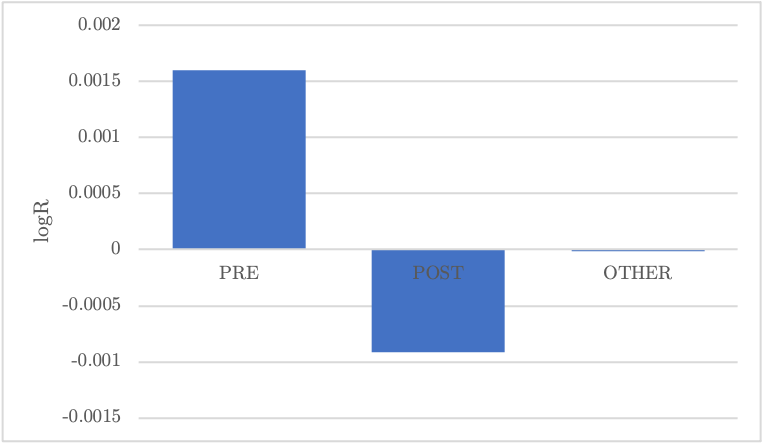
\includegraphics[width=9cm,height=5cm]{NAS-HE1.png} 
                \caption{NASDAQ Comprehensive Holiday Effect Mean Daily Returns}
        \end{center}
        \end{figure}

	Figure 19 shows evidence of the Holiday Effect theory in the NASDAQ, though not as explicitly as Figure 16 does, the NYSE. Pre-holidays hold the only positive mean and in that, also the greatest magnitude by \~{}67\%. Negative post-holidays support the Holiday Effect also.

	\begin{figure}[H]
        \begin{center}
                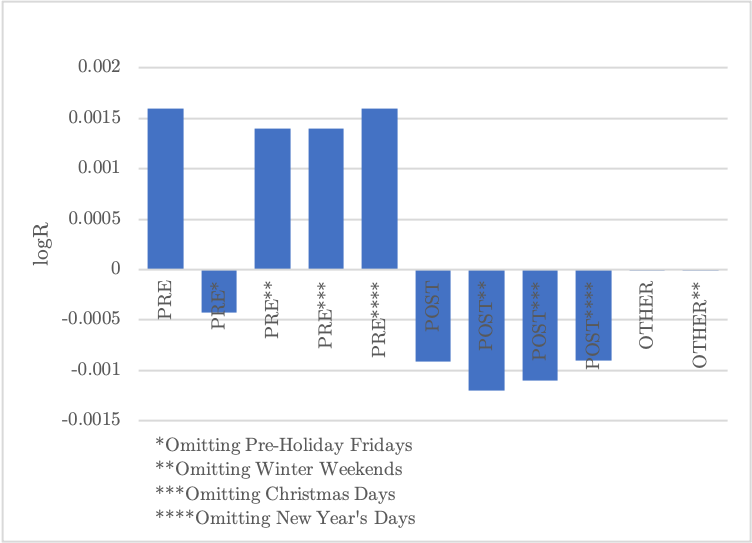
\includegraphics[width=9cm,height=5cm]{NAS-HE2.png}              
                \caption{NASDAQ Comprehensive Holiday Effect Mean Daily Returns H.E.E.} 
        \end{center}
        \end{figure}

	Figure 20 shows that the removal of pre-holiday Fridays has a similar effect to that of the NYSE’s. Pre-holiday average return becomes negative but not nearly as negative as that of the NYSE, only \~{}30\% of the magnitude. This again means many of the most valuable pre-holidays fall on Fridays. Omitting winter weekends reduces pre-holiday mean slightly and makes the post-holiday mean slightly more negative, meaning some high-return pre-holidays and some of the higher/positive post-holidays fall around winter weekends. Winter weekends hold an `inverse- post-holiday effect’ Omitting Christmas holidays has a very similar effect to winter weekends, with almost identical alterations. Meaning that Christmas periods hold this `inverse post-holiday effect’. Removing New Year has a negligible effect, likely meaning an even spread of positive/negative, high-magnitude/low-magnitude values were extracted in doing so.

	\begin{figure}[H]
        \begin{center}
                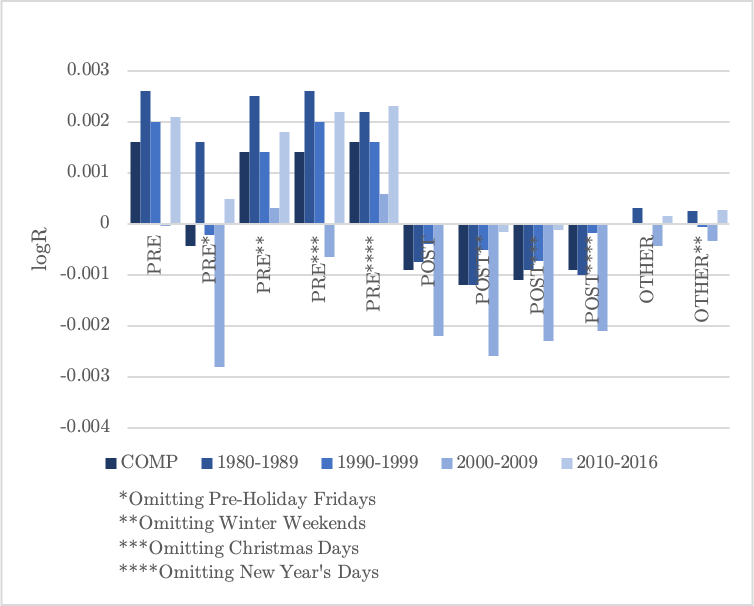
\includegraphics[width=9cm,height=5cm]{NAS-HE3.png}              
                \caption{NASDAQ Segmented Holiday Effect Mean Daily Returns H.E.E.}    
        \end{center}
        \end{figure}

	Once again, prior arguments are supported when segmented, in Figure 21. The negative Friday-removal pre-holidays are primarily driven by 2000-2009, with the greatest negativity and magnitude across-the-board. Thus, 2000-2009 contained the most positive pre-holiday Fridays. The removal of winter weekends, Christmas and New Year saw roughly the same trends as each-other; with 2000-2009 actually experiencing increases in pre-holiday means for removal of winter weekends and New Year, meaning they held lower pre-holiday returns in those days. 2000-2009 does however see a flip to negativity in removal of Christmas meaning they held higher pre-Christmas-holiday days. 2000-2009 also led in the biggest drop (increase in negativity) in post-holiday days, being up to 100\% larger than prior periods. This means 2000-2009 also held the highest (least-negative/most-positive) winter/Christmas/New Year post-holidays. There’s also evidence that the near-zero ‘other day’ returns aren’t caused by opposing skews etc. but simply higher/lower (not- zero) returns are found on pre/post-holiday days. Other days’ find consistent deviation from zero over the period.

	\newpage

	\begin{center}
                \scriptsize
        \begin{longtable}{ p{2cm} p{2cm} p{2cm} p{2cm} p{2cm} }
                & \textbf{coefficient} & \textbf{std.err} & \textbf{t-ratio} & \textbf{p-value}\\
                \hline
                \hline
                \multicolumn{5}{c}{\textbf{Standard}}\\
                \hline
                \hline
                \multicolumn{5}{c}{\textbf{Section I: Comprehensive}}\\
                \hline
                Pre-Hol & & & & \\
                Post-Hol & & & & \\
                Other Days & & & & \\
                \hline
                \multicolumn{5}{c}{\textbf{Section II: 1980--1989}}\\
                \hline            
                Pre-Hol & & & & \\ 
                Post-Hol & & & & \\  
                Other Days & & & & \\
                \hline
		\multicolumn{5}{c}{\textbf{Section III: 1990--1999}}\\
                \hline            
                Pre-Hol & & & & \\ 
                Post-Hol & & & & \\  
                Other Days & & & & \\
                \hline
                \multicolumn{5}{c}{\textbf{Section IV: 2000--2009}}\\
                \hline            
                Pre-Hol & & & & \\ 
                Post-Hol & & & & \\  
                Other Days & & & & \\
                \hline
                \multicolumn{5}{c}{\textbf{Section V: 2010--2016}}\\
                \hline            
                Pre-Hol & & & & \\ 
                Post-Hol & & & & \\  
                Other Days & & & & \\
                \hline
                \hline                                 
                \multicolumn{5}{c}{\textbf{Omitting Pre-Holiday Fridays}}\\         
                \hline
                \hline                                                 
                \multicolumn{5}{c}{\textbf{Section I: Comprehensive}}\\
                \hline            
                Pre-Hol & & & & \\ 
                Post-Hol & & & & \\  
                Other Days & & & & \\
                \hline                                          
                \multicolumn{5}{c}{\textbf{Section II: 1980--1989}}\\   
                \hline            
                Pre-Hol & & & & \\ 
                Post-Hol & & & & \\  
                Other Days & & & & \\
                \hline 
                \multicolumn{5}{c}{\textbf{Section III: 1990--1999}}\\   
                \hline            
                Pre-Hol & & & & \\ 
                Post-Hol & & & & \\  
                Other Days & & & & \\
                \hline 
                \multicolumn{5}{c}{\textbf{Section IV: 2000--2009}}\\   
                \hline                                          
                Pre-Hol & & & & \\
                Post-Hol & & & & \\  
                Other Days & & & & \\
                \hline 
                \multicolumn{5}{c}{\textbf{Section V: 2010--2016}}\\   
                \hline            
                Pre-Hol & & & & \\ 
                Post-Hol & & & & \\  
                Other Days & & & & \\
                \hline
                \hline
		\multicolumn{5}{c}{\textbf{Omitting Winter Weekends}}\\ 
                \hline
                \hline
                \multicolumn{5}{c}{\textbf{Section I: Comprehensive}}\\
                \hline
                Pre-Hol & & & & \\
                Post-Hol & & & & \\
                Other Days & & & & \\
                \hline
                \multicolumn{5}{c}{\textbf{Section II: 1980--1989}}\\
                \hline
                Pre-Hol & & & & \\
                Post-Hol & & & & \\  
                Other Days & & & & \\
                \hline 
                \multicolumn{5}{c}{\textbf{Section III: 1990--1999}}\\   
                \hline            
                Pre-Hol & & & & \\ 
                Post-Hol & & & & \\  
                Other Days & & & & \\
                \hline 
                \multicolumn{5}{c}{\textbf{Section IV: 2000--2009}}\\
                \hline                                          
                Pre-Hol & & & & \\
                Post-Hol & & & & \\  
                Other Days & & & & \\
                \hline 
                \multicolumn{5}{c}{\textbf{Section V: 2010--2016}}\\   
                \hline            
                Pre-Hol & & & & \\ 
                Post-Hol & & & & \\  
                Other Days & & & & \\
                \hline 
                \hline                                          
                \multicolumn{5}{c}{\textbf{Omitting Christmas Days}}\\ 
                \hline
                \hline
                \multicolumn{5}{c}{\textbf{Section I: Comprehensive}}\\
                \hline
                Pre-Hol & & & & \\
                Post-Hol & & & & \\
                Other Days & & & & \\
                \hline
                \multicolumn{5}{c}{\textbf{Section II: 1980--1989}}\\
                \hline
                Pre-Hol & & & & \\
                Post-Hol & & & & \\  
                Other Days & & & & \\
                \hline 
                \multicolumn{5}{c}{\textbf{Section III: 1990--1999}}\\   
                \hline            
                Pre-Hol & & & & \\ 
                Post-Hol & & & & \\  
                Other Days & & & & \\
		\hline 
                \multicolumn{5}{c}{\textbf{Section IV: 2000--2009}}\\
                \hline                                          
                Pre-Hol & & & & \\
                Post-Hol & & & & \\  
                Other Days & & & & \\
                \hline 
                \multicolumn{5}{c}{\textbf{Section V: 2010--2016}}\\   
                \hline            
                Pre-Hol & & & & \\ 
                Post-Hol & & & & \\  
                Other Days & & & & \\
                \hline 
                \hline                                          
                \multicolumn{5}{c}{\textbf{Omitting New Year's Days}}\\ 
                \hline
                \hline
                \multicolumn{5}{c}{\textbf{Section I: Comprehensive}}\\
                \hline
                Pre-Hol & & & & \\
                Post-Hol & & & & \\
                Other Days & & & & \\
                \hline
                \multicolumn{5}{c}{\textbf{Section II: 1980--1989}}\\
                \hline
                Pre-Hol & & & & \\
                Post-Hol & & & & \\  
                Other Days & & & & \\
                \hline 
                \multicolumn{5}{c}{\textbf{Section III: 1990--1999}}\\   
                \hline            
                Pre-Hol & & & & \\ 
                Post-Hol & & & & \\  
                Other Days & & & & \\
                \hline 
                \multicolumn{5}{c}{\textbf{Section IV: 2000--2009}}\\
                \hline                                          
                Pre-Hol & & & & \\
                Post-Hol & & & & \\  
                Other Days & & & & \\
                \hline 
                \multicolumn{5}{c}{\textbf{Section V: 2010--2016}}\\   
                \hline            
                Pre-Hol & & & & \\ 
                Post-Hol & & & & \\  
                Other Days & & & & \\
                \hline
                \multicolumn{5}{l}{$^*$: 10\% Significance Level}\\  
                \multicolumn{5}{l}{$^{**}$: 5\% Significance Level}\\ 
                \multicolumn{5}{l}{$^{***}$: 1\% Significance Level}\\
                \hline
                \caption{NASDAQ Holiday Effect Regression Results}
        \end{longtable}
        \end{center}

			\paragraph{Standard Observation}

			Table 5.17 highlights significantly positive pre-holiday days in all periods apart from 2000-2009. The greatest significance is seen in 1990-1999, at 1\% ; highlighting a coefficient stating pre-holidays result in a higher average return 0.002248 units, over other days. Thus, the null hypothesis is rejected with 95-99\% confidence across these periods. There is therefore, a present pre-holiday effect but no Holiday Effect as there is no significance in negative post-holidays.

			\paragraph{Omitting Pre-Holiday Fridays}

			Removal of pre-holiday Fridays sees all significant positivity removed. Two of the four coefficients which were once significantly positive, flip to negative. Although they aren’t significantly negative, they still support the argument that pre-holiday days’ significance is primarily held on Fridays. Recall, this is most apparent from 2000-2009 (Figure 21).

			\paragraph{Omitting Winter Weekends}

			The removal of winter weekends sees a slight drop in significance comprehensive; from 1\% to 5\% in a positive pre-holiday effect. All pre-holiday significance is also removed from the periods of 1990-1999 and 2010-2016. This means winter weekends hold significantly higher pre-holiday days in these times. There is no notable significant change in post-holidays although, they are made slightly more negative; significant at the 10\% level. This means winter weekend post-holiday do contain some slightly significantly higher returns – ‘inverse post-holiday effect’ in winter weekends. There is no significant change on `other’ days.

			\paragraph{Omitting Christmas Days}

			Removal of Christmas days does not have as significant an impact as winter weekends however, significance is dropped to 10\% from 5\%. This means that Christmas Day pre-holidays do in fact contain significantly higher returns also. The same argument in winter weekend post-holiday days holds for Christmas Day post-holidays, meaning they too contain an `inverse post-holiday effect’.

			\paragraph{Omitting New Year’s Days}

			Removal of New Year, like Christmas Days, sees a drop from 1\% to 5\% significance in positive pre-holidays. All of 2000-2009’s pre-holiday positive significance, once at the 5\% level, is removed. Thus, meaning New Year pre-holidays contain significantly higher returns in 2000-2009. There is no significant change in post-holidays.

		\subsubsection{The S\&P 500}

	\begin{figure}[H]
        \begin{center}
                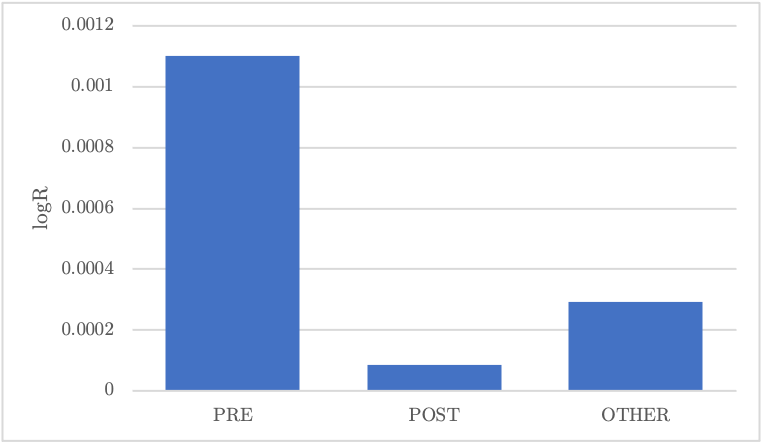
\includegraphics[width=9cm,height=5cm]{SP-HE1.png} 
		\caption{S\&P 500 Comprehensive Holiday Effect Mean Daily Returns}
        \end{center}
        \end{figure}

	Figure 22 highlights a large comprehensive pre-holiday effect; with pre-holiday mean return being \~{}260\% greater than that of other days. However, it is less than both NYSE and NASDAQ. Post-holidays do not support the Holiday Effect as their mean lies above zero, although it is only \~{}30\% of other days’.

	\begin{figure}[H]
        \begin{center}
                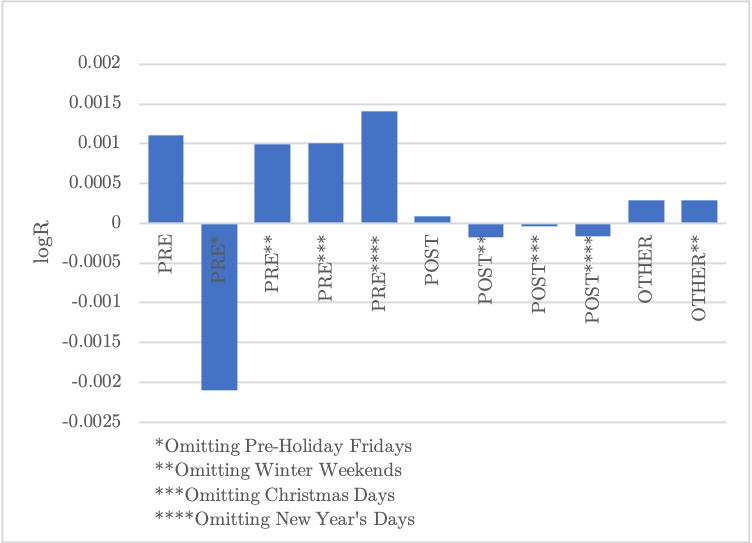
\includegraphics[width=9cm,height=5cm]{SP-HE2.png} 
		\caption{S\&P 500 Comprehensive Holiday Effect Mean Daily Returns H.E.E.}
        \end{center}
        \end{figure}

	Figure 23 shows that the removal of pre-holiday Fridays has the greatest effect in the S\&P 500, with pre-holiday return obtaining the greatest magnitude by \~{}33\% over the NYSE’s and, being by far more negative/positive than any other observation on the S\&P 500. This means the S\&P 500 contains the most abnormally valuable Fridays falling on pre-holiday days. Omitting winter weekends and Christmas Days has an approximately equal effect on pre-holiday Fridays in that their mean is slightly reduced; meaning a few higher-valued pre-holiday days fell in these periods. Both of these omissions, in addition to New Year omissions, also make post-holiday means less-than-zero; meaning some higher-valued post-holiday days were contained in those observations; `inverse-post-holiday effect’ contained in removed days. Removing New Year increases pre-holiday mean slightly; meaning some lower-valued pre-holidays were contained around New Year; `inverse-pre-holiday effect’ contained in removed days. Other days go observably-unaltered meaning near-mean or equally positive/negative `other-day’ winter weekends were removed.

	\begin{figure}[H]
        \begin{center}
                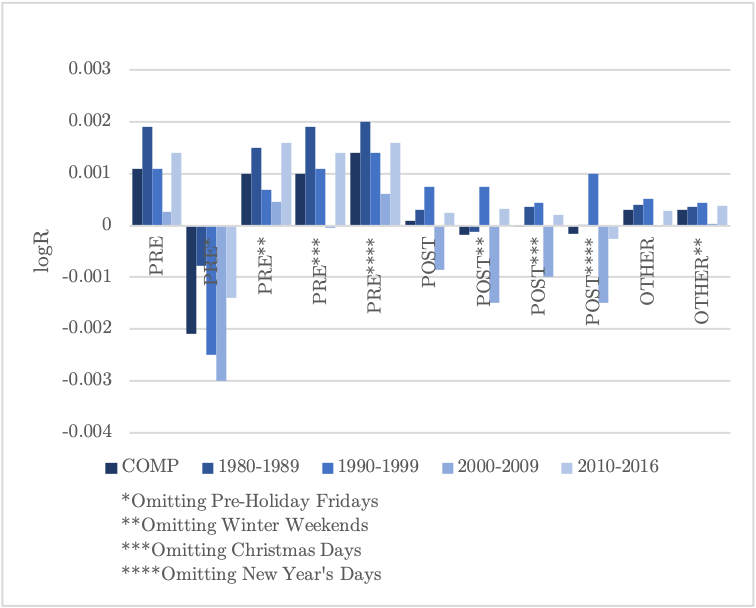
\includegraphics[width=9cm,height=5cm]{SP-HE3.png} 
		\caption{S\&P 500 Segmented Holiday Effect Mean Daily Returns H.E.E.}
        \end{center}
        \end{figure}

	Figure 24 shows the highest pre-holiday mean return in 1980-1989, in-line with the NYSE and NASDAQ. Pre-holiday means follow the trend of high-to-low in order: 1980-1989, 2010-2016, 1990-1999, 2000-2009 and hold this trend over removals of winter weekends, Christmas Days and New Year; meaning any effects these removals have work proportionately and don’t occur more-than-average at any given time. The aforementioned trend inverts in context of negativity when pre-holiday Fridays are removed (1980-1989 being least negative, 2000-2009 being most negative etc.); meaning again the effects of removing pre-holiday Fridays are consistent. Almost all of the negativity/flip-to-negativity in post-holiday days is contained within 2000-2016; there’s near-insignificant change the rest of the time; meaning the majority of higher- than-average post-holiday days are removed in 2000-2016. Other days follow a consistent trend across all amendments/periods.

	\newpage

	\begin{center}
                \scriptsize
        \begin{longtable}{ p{2cm} p{2cm} p{2cm} p{2cm} p{2cm} }
                & \textbf{coefficient} & \textbf{std.err} & \textbf{t-ratio} & \textbf{p-value}\\
                \hline
                \hline
                \multicolumn{5}{c}{\textbf{Standard}}\\
                \hline
                \hline
                \multicolumn{5}{c}{\textbf{Section I: Comprehensive}}\\
                \hline
                Pre-Hol & & & & \\
                Post-Hol & & & & \\
                Other Days & & & & \\
                \hline
                \multicolumn{5}{c}{\textbf{Section II: 1980--1989}}\\
                \hline            
                Pre-Hol & & & & \\ 
                Post-Hol & & & & \\  
                Other Days & & & & \\
                \hline
                \multicolumn{5}{c}{\textbf{Section III: 1990--1999}}\\
                \hline            
                Pre-Hol & & & & \\ 
                Post-Hol & & & & \\  
                Other Days & & & & \\
                \hline
                \multicolumn{5}{c}{\textbf{Section IV: 2000--2009}}\\
                \hline            
                Pre-Hol & & & & \\ 
                Post-Hol & & & & \\  
                Other Days & & & & \\
                \hline
                \multicolumn{5}{c}{\textbf{Section V: 2010--2016}}\\
                \hline            
                Pre-Hol & & & & \\ 
                Post-Hol & & & & \\  
                Other Days & & & & \\
                \hline
                \hline                                 
                \multicolumn{5}{c}{\textbf{Omitting Pre-Holiday Fridays}}\\
		\hline
                \hline                                                 
                \multicolumn{5}{c}{\textbf{Section I: Comprehensive}}\\
                \hline            
                Pre-Hol & & & & \\ 
                Post-Hol & & & & \\  
                Other Days & & & & \\
                \hline                                          
                \multicolumn{5}{c}{\textbf{Section II: 1980--1989}}\\   
                \hline            
                Pre-Hol & & & & \\ 
                Post-Hol & & & & \\  
                Other Days & & & & \\
                \hline 
                \multicolumn{5}{c}{\textbf{Section III: 1990--1999}}\\   
                \hline            
                Pre-Hol & & & & \\ 
                Post-Hol & & & & \\  
                Other Days & & & & \\
                \hline 
                \multicolumn{5}{c}{\textbf{Section IV: 2000--2009}}\\   
                \hline                                          
                Pre-Hol & & & & \\
                Post-Hol & & & & \\  
                Other Days & & & & \\
                \hline 
                \multicolumn{5}{c}{\textbf{Section V: 2010--2016}}\\   
                \hline            
                Pre-Hol & & & & \\ 
                Post-Hol & & & & \\  
                Other Days & & & & \\
                \hline
                \hline
                \multicolumn{5}{c}{\textbf{Omitting Winter Weekends}}\\
		\hline
                \hline
                \multicolumn{5}{c}{\textbf{Section I: Comprehensive}}\\
                \hline
                Pre-Hol & & & & \\
                Post-Hol & & & & \\
                Other Days & & & & \\
                \hline
                \multicolumn{5}{c}{\textbf{Section II: 1980--1989}}\\
                \hline
                Pre-Hol & & & & \\
                Post-Hol & & & & \\  
                Other Days & & & & \\
                \hline 
                \multicolumn{5}{c}{\textbf{Section III: 1990--1999}}\\   
                \hline            
                Pre-Hol & & & & \\ 
                Post-Hol & & & & \\  
                Other Days & & & & \\
                \hline 
                \multicolumn{5}{c}{\textbf{Section IV: 2000--2009}}\\
                \hline                                          
                Pre-Hol & & & & \\
                Post-Hol & & & & \\  
                Other Days & & & & \\
                \hline 
                \multicolumn{5}{c}{\textbf{Section V: 2010--2016}}\\   
                \hline            
                Pre-Hol & & & & \\ 
                Post-Hol & & & & \\  
                Other Days & & & & \\
                \hline 
                \hline                                          
                \multicolumn{5}{c}{\textbf{Omitting Christmas Days}}\\
		\hline
                \hline
                \multicolumn{5}{c}{\textbf{Section I: Comprehensive}}\\
                \hline
                Pre-Hol & & & & \\
                Post-Hol & & & & \\
                Other Days & & & & \\
                \hline
                \multicolumn{5}{c}{\textbf{Section II: 1980--1989}}\\
                \hline
                Pre-Hol & & & & \\
                Post-Hol & & & & \\  
                Other Days & & & & \\
                \hline 
                \multicolumn{5}{c}{\textbf{Section III: 1990--1999}}\\   
                \hline            
                Pre-Hol & & & & \\ 
                Post-Hol & & & & \\  
                Other Days & & & & \\
                \hline 
                \multicolumn{5}{c}{\textbf{Section IV: 2000--2009}}\\
                \hline                                          
                Pre-Hol & & & & \\
                Post-Hol & & & & \\  
                Other Days & & & & \\
                \hline 
                \multicolumn{5}{c}{\textbf{Section V: 2010--2016}}\\   
                \hline            
                Pre-Hol & & & & \\ 
                Post-Hol & & & & \\  
                Other Days & & & & \\
                \hline 
                \hline                                          
                \multicolumn{5}{c}{\textbf{Omitting New Year's Days}}\\
		\hline
                \hline
                \multicolumn{5}{c}{\textbf{Section I: Comprehensive}}\\
                \hline
                Pre-Hol & & & & \\
                Post-Hol & & & & \\
                Other Days & & & & \\
                \hline
                \multicolumn{5}{c}{\textbf{Section II: 1980--1989}}\\
                \hline
                Pre-Hol & & & & \\
                Post-Hol & & & & \\  
                Other Days & & & & \\
                \hline 
                \multicolumn{5}{c}{\textbf{Section III: 1990--1999}}\\   
                \hline            
                Pre-Hol & & & & \\ 
                Post-Hol & & & & \\  
                Other Days & & & & \\
                \hline 
                \multicolumn{5}{c}{\textbf{Section IV: 2000--2009}}\\
                \hline                                          
                Pre-Hol & & & & \\
                Post-Hol & & & & \\  
                Other Days & & & & \\
                \hline 
                \multicolumn{5}{c}{\textbf{Section V: 2010--2016}}\\   
                \hline            
                Pre-Hol & & & & \\ 
                Post-Hol & & & & \\  
                Other Days & & & & \\
                \hline
                \multicolumn{5}{l}{$^*$: 10\% Significance Level}\\  
                \multicolumn{5}{l}{$^{**}$: 5\% Significance Level}\\ 
                \multicolumn{5}{l}{$^{***}$: 1\% Significance Level}\\
                \hline
		\caption{S\&P 500 Holiday Effect Regression Results}
        \end{longtable}
        \end{center}

			\paragraph{Standard Observation}

			Table 5.18 highlights no cases of significantly positive pre-holiday observations or significantly negative post-holiday observations. Thus, there is no Holiday Effect present. The furthest from the Holiday Effect is 1990-1999, with non-pre/post-holiday days being the significant driver of positive returns in that period; at the 1\% significant level. Therefore, the null hypothesis is failed-to-be-rejected stating that returns on observed days (pre/post-holidays) are not significantly different from those of other days.

			\paragraph{Omitting Pre-Holiday Fridays}

			Removal of pre-holiday Fridays sees pre-holiday days comprehensively go from insignificant (actually 10\% level) to negative at the 1\% significance level. This is primarily driven by 1990-1999’s pre-holiday significant negativity at the 5\% level and the introduction of significant negativity at the 10\% level in 2000-2009. All coefficients, including insignificant ones, are indeed flipped to negative. Thus, the S\&P 500 supports the argument that pre-holiday days’ significance is primarily held on Fridays.

			\paragraph{Omitting Winter Weekends}

			The removal of winter weekends first, removes comprehensive significance in pre- holiday days but this was only relevant at the 10\% level. It does mean though that winter weekends contain marginally higher pre-holiday returns in this observation. Primarily, winter weekend removal lowers `other’ day positive significance in 1990- 1999 meaning non-pre/post-holiday winter weekend days were marginally higher in that period. And, it adds `other’ day positive significance in 2010-2016 meaning non- pre/post-holiday winter weekend days were marginally lower in that period. There is no significant change on `other’ days. There is no significant post-holiday change.

			\paragraph{Omitting Christmas Days}

			Removal of Christmas Days does not have any significant effect on pre-holiday or post-holiday returns, in any period. Significance and coefficients remain the same as the standard observation’s.

			\paragraph{Omitting New Year’s Days}

			The removal of New Year has a slight impact in the comprehensive positive significance of pre-holidays. Significance increases from 10\% to 5\%, caused by a fairly even spread of lower-return pre-New-Year-holidays across the segmented periods, as there is no significant spike in any particular period. This therefore means that, although it does not align with the expectation that pre-New-Year-holidays would be higher, the pre-holiday effect would be determined present in the S\&P 500, given the disappearance of New Year.

	\newpage

	\subsection{Measures of Model Integrity}

	Models within this study use only variables which are products of correspondence with one set of values (in their relative model). Therefore, tests such as R$^2$ observation, omitted variable bias, information criteria, f-tests, RESET tests, endogeneity tests are irrelevant as an `optimal model’ with `optimal variables’ is not sought. There is simply observation of correspondence. All tests are outlined in full, in Figure B3, for your leisure. Below, in Tables 5.19 and 5.20, heteroscedasticity `White’ test and unit-root `Dickie-Fuller’ test results are displayed respectively. Accounting for the models with Holiday Effect omissions is irrelevant; not included.

	\begin{table}[h]
		\scriptsize
	\begin{center}
	\begin{tabular}{ p{2.25cm} p{2.25cm} p{2.25cm} p{2.25cm} p{2.25cm} }
		\textbf{Comprehensive} & \textbf{1989--1989} & \textbf{1990--1999} & \textbf{2000--2009} & \textbf{2010--2016}\\
		\hline
		\hline
		\multicolumn{5}{c}{\textbf{Weekend Effect Models}}\\
		\hline
		\hline
		\multicolumn{5}{c}{\textbf{NYSE Composite p-values}}\\
		\hline
		0.070120 & 0.656886 & 0.060085 & 0.200971 & 0.987515\\
		\hline
		\multicolumn{5}{c}{\textbf{NASDAQ Composite p-values}}\\
		\hline
		0.321306 & 0.254783 & 0.052530 & 0.407484 & 0.955632\\
		\hline
		\multicolumn{5}{c}{\textbf{S\&P 500 p-values}}\\
		\hline
		0.087312 & 0.792264 & 0.070942 & 0.390712 & 0.967437\\
		\hline
		\hline
		\multicolumn{5}{c}{\textbf{January Effect Models}}\\
                \hline
                \hline
                \multicolumn{5}{c}{\textbf{NYSE Composite p-values}}\\
		\hline
		0.320315 & 0.225796 & 0.285982 & 0.548384 & 0.092961\\
		\hline
		\multicolumn{5}{c}{\textbf{NASDAQ Composite p-values}}\\
		\hline
		0.387380 & 0.097319 & 0.307185 & 0.485721 & 0.413817\\
		\hline 
		\multicolumn{5}{c}{\textbf{S\&P 500 p-values}}\\
		\hline
		0.073835 & 0.223072 & 0.182985 & 0.447122 & 0.059895\\
		\hline
		\hline
		\multicolumn{5}{c}{\textbf{Holiday Effect Models}}\\
		\hline
		\hline
		\multicolumn{5}{c}{\textbf{NYSE Composite p-values}}\\
		\hline
		0.360840 & 0.845632 & 0.316595 & 0.302404 & 0.868398\\
		\hline
                \multicolumn{5}{c}{\textbf{NASDAQ Composite p-values}}\\
		\hline
		0.064794 & 0.553657 & 0.303319 & 0.123635 & 0.135701\\
		\hline
                \multicolumn{5}{c}{\textbf{S\&P 500 p-values}}\\
		\hline
		0.421098 & 0.798743 & 0.287562 & 0.367225 & 0.821357\\
		\hline
	\end{tabular}
		\caption{Heteroscedasticity `White' Test Results}
	\end{center}
	\end{table}

	Again, all variables are products of correspondence with one set of values (in their relative model). Given this and the type of model usen, no heteroscedasticity issues should be present. Table 5.19 displays evidence that there is no heteroscedasticity present in any model, finding consistent p-values which are all over 0.05. Therefore, in all cases, the null hypothesis that there is homoscedasticity present (constant error terms) is failed-to-be-rejected.

	\begin{table}[h]
		\scriptsize
	\begin{center}
	\begin{tabular}{ p{3.5cm} p{3.5cm} p{3.5cm} }
		\textbf{NYSE Composite} & \textbf{NASDAQ Composite} & \textbf{S\&P 500}\\
		\hline
		\multicolumn{3}{c}{\textbf{Daily Returns p-values}}\\
		\hline
		3.663e-37 & 2.642e-35 & 3.247e-36\\
		\hline
		\multicolumn{3}{c}{\textbf{Monthly Returns p-values}}\\
		\hline
		6.5e-35 & 9.315e-35 & 1.212e-35\\
		\hline
	\end{tabular}
		\caption{Unit-Root `Dickie-Fuller’ Test Results}
	\end{center}
	\end{table}

	Table 5.20 shows that there are no unit-roots present in any model, finding consistent p-values which are all significantly below 0.05. Therefore, in all cases, the null hypothesis that there is non-stationarity, unit-roots, is rejected with 99\% confidence. The alternative hypothesis that there is stationarity and no unit-roots is favoured.

	\newpage 

	\subsection{Question \& Answer Summary}

	\begin{table}[h]
        \begin{center}
        	\scriptsize
        \begin{tabular}{ l l l }
        	\textbf{Question} & & \textbf{Status} \\ 
        	\hline
        	\textbf{Q1} & \textbf{Does Fama’s (1970) EMH hold in empirical evidence?} & Partial\\
                \textbf{Q2} & \textbf{Is the Seasonal Effect apparent in the US Market?} & Partial\\
        	Q2.1 & Does the Weekend Effect exist? & Partial\\
                Q2.2 & Does the January Effect exist? & Partial\\
                Q2.3 & Does the Holiday Effect exist? & Partial\\
                \textbf{Q3} & \textbf{Do internal patterns influence Abnormal Returns?} & Partial\\
                Q3.1 & Is the Holiday Effect significantly influenced by pre-holiday Fridays? & Yes\\
                Q3.2 & Is the Holiday Effect significantly influenced by winter weekends? & Partial\\
                Q3.3 & Is the Holiday Effect significantly influenced by Christmas Day? & Partial\\
                Q3.4 & Is the Holiday Effect significantly influenced by New Year? & No\\
                \textbf{Q4} & \textbf{Are methods in this research relevant?} & Yes\\
                Q4.1 & Do up-to-date-sample results differ from those of past research? & Yes\\
                Q4.2 & Do results significantly differ over indices? & Yes\\
                Q4.3 & Do results significantly differ over time-period segments? & Yes\\
                \hline
                Yes/No: & There is/is no significant evidence in past research and current observations \\
                Partial: & There is inconsistent significant evidence in past research and current observations \\
                TBD/...: & To Be Discussed/Being Discussed \\
                \hline
        \end{tabular}                            
                \caption {Questions (Chapter 5 Update)}
        \end{center}
	\end{table}

	Table 5.21 evises questions. In result, it would be difficult to say that Fama’s (1970) EMH holds in empirical evidence. Much like previous literature, evidence of the Weekend Effect, the January Effect and the Holiday Effect is found, frequently in partial components, sometimes in the correct trends but not significant enough to be determined noteworthy. The removal of pre-holiday Fridays does have a consistent effect on pre-holidays; removing any pre-holiday effect and making pre-holiday returns negative in all observations. Removal of winter weekends has some effect on the removal of any pre-holiday effect however, this is inconsistent over time and indices. The omission of Christmas Days and New Year’s Days has a similar but, again, inconsistent effect. Although similar evidence holds with regards to past research, the up-to-date and segmented sample used shows various factors diminish towards the present day.

\newpage 
% Conclusion

	\section{Research Conclusions}

	\subsection{Does Fama’s (1970) EMH Hold In Practice?}

	In the foundation of the US stock market, intensions of investors were as pure as they would have ever been. They sought the closest outcomes to ones as described by Fama; in fully-reflective prices, fair values, passive portfolios. Portfolios followed a risk- seeking/risk-averse pattern, in-line with Fama’s argument of higher-risk, higher- payoff. To this day, Fama’s outline has loosened. ``Historical prices are irrelevant..." is untrue in 2020. Previous literature and this study has reinforced the fact that there are patterns in seasonal stock returns. As always, these are never a given; `written-in- stone’, if you will. This information may be ``financially costless/available" but, these patterns do not reflect ``certain and agreed upon prices" (Fama, 1970). They are persistent but not reliable, meaning that they aren’t entirely irrelevant when predicting future prices, as Fama describes, but their stability has lost-grip in recent years and they’re becoming a less-reliable way for investors to react. If there is a peak in `disagreement’ with Fama’s arguments, it’s visible mostly in the mid-to-late 1900’s. Even the Seasonal Effect is becoming far more in-line with `luck’.

	\newpage

	\subsection{Is the Seasonal Effect Present in the US Market?}

	Following headings are named according to Q2 and Q3. Conclusions are made considering the unlisted Q4. Recall:\\

	\textbf{Q4 Are methods in this research relevant?}\\ Q4.1 Do up-to-date-sample results differ from those of past research?\\ Q4.2 Do results significantly differ over indices?\\ Q4.3 Do results significantly differ over time-period segments?

		\subsubsection{Does the Weekend Effect Exist?}

		The Weekend Effect exists partially. Most frequently, only the Monday Effect is present, with only one case of the full Weekend Effect. In-line with Keim and Stambaugh (1984), partial evidence is found in the S\&P 500. This is extended to the NYSE and NASDAQ and does show reason for including multiple indices in that, the NASDAQ shows the full Weekend Effect in 1980-1989 and, an overall/comprehensive Monday Effect. This differs from the NYSE and S\&P 500 which include only 1980- 1989/1990-1999 Monday Effects. From this it’s also clear that the time-period- segmentation are effective, showing the Weekend/Monday Effect diminishes over time. The NASDAQ shows the most negative Monday returns and the most consistent negative returns. They are negative until 2010-2016, after which they are still barely positive. The NYSE and S\&P 500 see positivity after 1990-1999 meaning their Monday Effect is lost. The NASDAQ’s full Weekend Effect also comes early in 1980-1989, supporting the former. It continues to support Weekend Effect trends longer than the other two indices, though not significantly.

		\subsubsection{Does the January Effect Exist?}

		The January Effect exists partially. This is said at a long stretch as it only appear in one period, 1990-1999 in the NASDAQ. The NASDAQ is the only index in which January is amongst the group which holds the highest returns. Rozeff and Kinney (1976) also find evidence over a long seventy-year period however, suggest that it is diminishing. The fact that, succeeding Rozeff and Kinney’s literature, the only observation here is in one period and one index shows that a once-visible January Effect has indeed died off. Thus, making the use of time-period-segmentations useful. The use of multiple indices however, does show there is more January Effect evidence around different types of investors/firms within the NASDAQ. Although from 2000, the NASDAQ’s January returns have too, become consistently negative. The January Effect is the least evident, persistent and stable factor in this study.

		\subsubsection{Does the Holiday Effect Exist?}

		The Holiday Effect exists partially. The Holiday Effect exists only in the form of the pre-holiday effect, in all observations. This aligns with Kim and Park’s (1994) observations of the NYSE and NASDAQ, on a more up-to-date basis. Pre-holiday returns are generally most positive in the NASDAQ and post-holiday returns are generally the most negative. This aligns with the persistence of the pre-holiday effect throughout almost periods in the NASDAQ, showing no sign of dying off. Thus, the NASDAQ highlights the most `predictable’ opportunity for positive abnormal returns. Meaning, investment factors aligned with the Holiday Effect are most apparent in more advancing, innovative, sometimes newer firms. This suggests that the Holiday Effect could continue to be persistent in firms of types such as those listed on the NASDAQ but, not within some older, more traditional and less growth-oriented firms. All of the former shows the effectiveness of utilising all three indices. The NYSE and S\&P 500 may show similar trends but nothing significant. They could still be argued as being ‘predictable’ however, returns may not be significant.

	\newpage

	\subsection{What Drives Abnormal Returns?}

		\subsubsection{Is the Holiday Effect Significantly Influenced By Pre-Holiday Fridays?}

		Pre-holiday Fridays influence pre-holidays. Liano, et al. (1992) suggest there’s a pattern in pre-holiday Fridays being the most profitable. Some evidence is provided but no definitive answer. This study shows persistent evidence across all indices and all time periods that removing pre-holiday Fridays makes pre-holiday returns hypothetically negative. There are only two cases in which this didn’t happen, both of which did still see a drop in positivity. The S\&P 500 saw the greatest negativity and the NASDAQ saw the most uncertainty over this amendment. The hypothetical case of the inverse-pre-holiday effect on pre-holidays means pre-holiday Fridays contain the most significant pre-holiday effect. We know there is a lack of the Friday Effect in this study meaning that if there was a Friday Effect, all Fridays would have to be pre-holidays. Thus, the majority of significantly positive Fridays fall on pre- holidays. The pre-holiday effect drives any Friday Effect that may be present on a smaller scale, e.g. when observing weekly/monthly intervals. This aligns well with expectations of this study and projections of Liano, et al. (1992). Finding a greater effect than Liano, et al., who only find a halving of pre-holiday magnitude.

		\subsubsection{Is the Holiday Effect Significantly Influenced By Winter Weekends?}

		Winter weekends influence pre-holidays, to some degree. In the same fashion as pre- holiday Fridays, winter weekends tend to hold slightly above-average-return pre- holidays. However, these are only high enough to remove significance from two periods across one index. Although the trend does agree with Kim and Park’s (1994) suggestion around amplified investor behaviour at the winter holiday period, there’s not enough significance to make any definitive conclusions.

		\subsubsection{Is the Holiday Effect Significantly Influenced By Christmas Days?}

		Christmas Days do not influence pre/post-holidays, to a significant degree. Across all indices and most time-periods, again, their removal has a similar effect to that of winter weekends; two periods of pre-holiday significance is removed, in one index. The trend again does align with the expectations of Christmas Day holidays holding above- average pre-holidays. There’s not much to be said regarding post-holidays.

		\subsubsection{Is the Holiday Effect Significantly Influenced By New Year?}

		New Year does not influence pre/post-holidays, to a significant degree. Their removal has the same effect as that of Christmas, with the trend again aligning with expectation, just not to a greatly significant degree. Their notable contribution is the hypothetical creation of the pre-holiday effect in the S\&P 500, upon removal. Meaning in that case, they contradict expectations in their lower-than-average pre-holiday values.

	\newpage

	\subsection{Final Notes}

	The Monday Effect is more evident than the Friday Effect. The January Effect is barely present. The pre-holiday effect is more evident than the post-holiday effect, any post-holiday effect/post-holiday change after amendment is too insignificant to draw certain conclusions. Pre-holiday Fridays drive positive pre-holiday abnormal returns. The Holiday Effect drives any smaller-scale Friday Effect. Winter weekends, Christmas and New Year contain primarily higher pre-holidays than other holidays, although majorly insignificantly so. Results support findings and suggestions/projections from past literature. Effects are usually more evident in a single index. All effects diminish over time apart from the NASDAQ’s pre-holiday effect.\\

	Yes, the Seasonal Effect exists but does this mean Fama’s idea of abnormal returns only being present under `luck’ is completely irrelevant? No, of course not. Seasonal patterns may be predictable to a degree however, there is a significantly lacking foundation for their integrity. Investor behaviour is unpredictable and just because investors have historically shown consistent seasonal patterns and changes in behaviour, circumstances could still change at any moment. If there was more rationale behind the Seasonal Effect, it could be a consistently reliable investment strategy but, like most financial patterns, it’s simply another futile theoretical overstatement.

\newpage
% Appendices

	\pagenumbering{Roman}

	\section*{Appendices}

\end{document}
